\documentclass[11pt]{article}
%\usepackage{fullpage,subfigure,fancyhdr}
\usepackage{color}
\usepackage{textcomp}
\usepackage{verbatim}
\usepackage{times}
\usepackage{amsfonts,amsmath,amssymb,amsthm}
\usepackage{textcomp}
\usepackage{url}
\usepackage{mdwlist}
\usepackage{wrapfig,caption,subfigure,sidecap}
\usepackage{xspace}
\usepackage{algorithm}
\usepackage{algpseudocode}
\usepackage{graphicx}
\usepackage[colorlinks=true,pagebackref,linkcolor=magenta]{hyperref}
\usepackage[sort&compress,comma,square,numbers]{natbib}
\usepackage{pict2e}
\usepackage[nottoc,numbib]{tocbibind}
\usepackage{paralist}
\usepackage{multicol}
\usepackage{lettrine}
\usepackage{helvet}
\usepackage{authblk}
\usepackage[linecolor=dark_blue, linewidth=1.5pt, skipabove=4pt, nobreak=true]{mdframed}
\usepackage{tikz}
\usepackage{graphicx}
\usepackage{neurodata}
% \usepackage{trackchanges}
% \usepackage{mcode}

\renewcommand{\familydefault}{\sfdefault}
\definecolor{MyGray}{rgb}{0.7,0.7,0.7}

% \numberwithin{figure}{section}
% \numberwithin{table}{section}
% \numberwithin{algorithm}{section}

% \pagestyle{fancy}
% \oddsidemargin=-0.5in 
% \evensidemargin=-0.5in
\textwidth=6.5in 
\headwidth=6.5in
\textheight=9.0in 
\headheight=0.0pt
\topmargin=0.0in
\headsep=0.0in
\renewcommand{\headrulewidth}{0pt}

\setlength{\parindent}{0em}
\setlength{\parskip}{0.5em}

%%%%% COLOR STUFF %%%%%%%%%%
\newcommand{\db}[1]{{\color{dark_blue}{#1}}}
\newcommand{\bb}[1]{{\textbf{\db{#1}}}}
\newcommand{\cb}[1]{\centering{{\textbf{\db{#1}}}}}

\definecolor{MyPlum}{rgb}{0.3,0,0.3}
\definecolor{MyOrange}{rgb}{1,0.5,0}
\definecolor{deep_blue}{rgb}{0,.2,.5}
\definecolor{dark_blue}{rgb}{0,.15,.5}

\newcommand{\marta}[1]{{\color{red}{\it marta: #1}}}
\newcommand{\youngser}[1]{{\color{green}{\it youngser: #1}}}
\newcommand{\brett}[1]{{\color{blue}{\it brett says: #1}}}
\newcommand{\jovo}[1]{{\color{magenta}{\it JoVo: #1}}}
\newcommand{\rb}[1]{{\color{red}{\it rb: #1}}}
\newcommand{\bro}[1]{{\color{blue}{\it youngser: #1}}}
\newcommand{\agastya}[1]{{\color{red}{\it agastya: #1}}}
\providecommand{\tg}[1]{\textcolor{green}{#1}}
\providecommand{\tb}[1]{\textcolor{blue}{#1}}
\providecommand{\tr}[1]{\textcolor{red}{#1}}
\providecommand{\tk}[1]{\textcolor{black}{#1}}
\providecommand{\twhite}[1]{\textcolor{white}{#1}}

\newcommand{\Linefor}[2]{%
    \State \algorithmicfor\ {#1}\ \algorithmicdo\ {#2} \algorithmicend\ \algorithmicfor%
}
\newcommand{\Lineif}[2]{%
    \State \algorithmicif\ {#1}\ \algorithmicdo\ {#2} \algorithmicend\ \algorithmicif%
}


%%%%%%%%% MATH OPERATORS %%%%%%%%%%%%
\providecommand{\ve}[1]{\boldsymbol{#1}}
\providecommand{\ma}[1]{\boldsymbol{#1}}
\providecommand{\norm}[1]{\left \lVert#1 \right  \rVert}
\providecommand{\deter}[1]{\lvert #1 \rvert}
\providecommand{\abs}[1]{\left \lvert #1 \right \rvert}
\providecommand{\mat}[1]{\left[ #1 \right]}
\newcommand{\trans}[1]{{#1}^{\ensuremath{\mathsf{T}}}}           % transpose
\newcommand{\transpose}[1]{{#1}^{\ensuremath{\mathsf{T}}}}           % transpose
\newcommand{\argmax}{\operatornamewithlimits{argmax}}
\newcommand{\argmin}{\operatornamewithlimits{argmin}}
\newcommand{\T}{^{\ensuremath{\mathsf{T}}}}           % transpose
\newcommand{\from}{{\ensuremath{\colon}}}           % :
\newcommand{\trace}[1]{{\ensuremath{\operatorname{tr}\!\left(#1\right)}}}           % :

\providecommand{\ms}[1]{\mathsf{#1}}
\providecommand{\mc}[1]{\mathcal{#1}}
\providecommand{\mt}[1]{\widetilde{#1}}
\providecommand{\mb}[1]{\boldsymbol{#1}}
\providecommand{\mbb}[1]{\mathbb{#1}}
\providecommand{\mv}[1]{\vec{#1}}
\providecommand{\mh}[1]{\hat{#1}}
\providecommand{\wh}[1]{\widehat{#1}}
\providecommand{\mhv}[1]{\mh{\mv{#1}}}
\providecommand{\mvh}[1]{\mv{\mh{#1}}}
\providecommand{\mhc}[1]{\hat{\mathcal{#1}}}
\providecommand{\mbc}[1]{\mb{\mathcal{#1}}}
\providecommand{\mvc}[1]{\mv{\mathcal{#1}}}
\providecommand{\mtc}[1]{\widetilde{\mathcal{#1}}}
\providecommand{\mth}[1]{\mt{\mh{#1}}}
\providecommand{\mht}[1]{\mh{\mt{#1}}}
\providecommand{\mhb}[1]{\hat{\boldsymbol{#1}}}
\providecommand{\whb}[1]{\widehat{\boldsymbol{#1}}}
\providecommand{\mvb}[1]{\vec{\boldsymbol{#1}}}
\providecommand{\mtb}[1]{\widetilde{\boldsymbol{#1}}}
\providecommand{\mbt}[1]{\widetilde{\boldsymbol{#1}}}
\providecommand{\mvc}[1]{\vec{\mathcal{#1}}}
% \newcommand{\D}[2]{\frac{\partial #1}{\partial #2}}
\newcommand{\dd}[2]{\frac{\partial ^2 #1}{\partial #2 ^2}}
\newcommand{\DDD}[3]{\frac{\partial ^2 #1}{\partial #2 \partial #3}}
\newcommand{\Di}[2]{\frac{\partial ^i #1}{\partial #2 ^i}}



%%%%%%%%%% ENVIRONMENTS %%%%%%%%%%%%%

\newtheorem{Rem}{Remark}%[section]
\newtheorem{Alg}{Algorithm}%[section]
\newtheorem{thm}{Theorem}
\newtheorem{Thm}{Theorem}[section]
\newtheorem{lem}{Lemma}
\newtheorem{Lem}{Lemma}%[section]
\newtheorem{defi}{Definition}
\newtheorem{Def}{Definition}[section]
\newtheorem{prop}{Proposition}
\newtheorem{coro}[thm]{Corollary}
\newtheorem{claim}{Claim}
\newtheorem{conj}{Conjecture}
\newtheorem{question}{Question}
\newtheorem{answer}{Answer}
\newtheorem{rem}{Remark}%[section]
\newtheorem{cor}[lem]{Corollary}
\newtheorem{model}{Model}
\newtheorem{remark}{Remark}

\newcommand{\bla}{\begin{block}}
\newcommand{\blb}{\end{block}}

\newcommand{\defa}{\begin{defi}}
\newcommand{\defb}{\end{defi}}
\newcommand{\theHalgorithm}{\arabic{algorithm}}

\newcommand{\thma}{\begin{thm}}
\newcommand{\thmb}{\end{thm}}

\newcommand{\mata}{\begin{bmatrix}}
\newcommand{\matb}{\end{bmatrix}}

\floatname{algorithm}{Procedure}
\renewcommand{\algorithmicrequire}{\textbf{Input:}}
\renewcommand{\algorithmicensure}{\textbf{Output:}}
\floatname{algorithm}{Pseudocode}



%%%%%%%%%% SECTIONS & STUFF %%%%%%%%%%%%%


\renewcommand{\thesection}{\Roman{section}}   % set the section counter to Alpha
\renewcommand{\thesubsection}{\Roman{section}.\Alph{subsection}}   % set the subsection counter to alpha
\renewcommand{\thesubsubsection}{\Roman{section}.\Alph{subsection}(\arabic{subsubsection})}   % set the subsection counter to alpha
% 
% 
\makeatletter
% \def\subsize{\@setsize\subsize{8pt}\xipt\@xipt}
 \def\section{\@startsection {section}{1}{\z@}{5pt}{9pt}{\Large\bf\db}}
 \def\subsection{\@startsection {subsection}{2}{\z@}{10pt}{4pt}{\large\bf\db}}
 \def\subsubsection{\@startsection {subsubsection}{2}{\z@}{10pt}{4pt}{\bf\db}}
% \def\subs{\@startsection {subsubsection}{2}{0pt}{5pt}{0pt}{ \subsize\bf\db}}
\def\paragraph{\@startsection {paragraph}{2}{\z@}{10pt}{4pt}{\bf\db}}
% \def\subparagraph{\@startsection 


\newcommand{\para}[1]{\vspace{3pt}\noindent{{\fontsize{10pt}{0pt}\bf\db{#1}}}}
\newcommand{\subpara}[1]{\vspace{3pt}\noindent{{\fontsize{10pt}{4pt} \bf \emph{#1}}}}
\newcommand{\subsubpara}[1]{\vspace{3pt}\noindent{{\fontsize{10pt}{4pt} \emph{#1}}}}

\setlength{\parindent}{0pt}



%%%%%% SHORT HAND %%%%%%%%%%
\renewcommand{\refname}{References and Notes}

\newcommand{\jv}{Joshua Vogelstein}

\newcommand{\Vr}{V_{reset}}
\newcommand{\Vl}{V_{leat}}
\newcommand{\eqdef}{\overset{\triangle}{=}}
\newcommand{\grad}{\nabla}
\newcommand{\Hess}{\nabla\nabla}
\newcommand{\defn}{\overset{\triangle}{=}}

\newcommand{\rto}{\leftarrow}
\newcommand{\iid}{\overset{iid}{\sim}}
\newcommand{\knn}{$k$NN}

\newcommand{\elegans}{\emph{C. elegans} }

\newcommand{\Lik}{\mathcal{L}}
\newcommand{\Cae}{[\widehat{\text{Ca}}^{2+}]}
\newcommand{\Cav}{\ve{C}}%[\ve{\text{Ca}}^{2+}]}
\newcommand{\sml}{\sqrt{\ma{\lambda}}}
\newcommand{\ml}{\ma{\lambda}}
\newcommand{\nw}{\widehat{n}}
\newcommand{\nv}{\vec{n}}
\newcommand{\Ae}{\widehat{A}}
\newcommand{\te}{\widehat{\tau}}
\newcommand{\maxn}{\max_{\ve{n}: n_t \geq 0}}
% \newcommand{\V}{\text{Var}}

\newcommand{\PmcP}{P \in \mc{P}}
\newcommand{\mP}{\mathbb{P}}

% \newcommand{\dvs}{\dot{\bs}_t}
% \newcommand{\dvw}{\dot{\bw}_t}
% \newcommand{\dvx}{\dot{\bx}_t}
% \newcommand{\dvy}{\dot{\by}_t}

\newcommand{\ft}{f_{\ve{\thet}}}
\newcommand{\gt}{g_{\ve{\thet}}}
\newcommand{\hht}{h_{\thetn}}

\newcommand{\Real}{\mathbb{R}}

\newcommand{\wconv}{\overset{i.p.}{\rightarrow}}
\newcommand{\sconv}{\overset{i.p.}{\rightarrow}}
\newcommand{\conv}{\rightarrow}
\newcommand{\pconv}{\overset{p}{\conv}}
\newcommand{\mcE}{\mathcal{E}}
\newcommand{\mcT}{\mathcal{T}}
\newcommand{\mcG}{\mathcal{G}}
\newcommand{\mcM}{\mathcal{M}}
\newcommand{\mcL}{\mathcal{L}}
\newcommand{\hatmcE}{\widehat{\mcE}}
\newcommand{\hatp}{\widehat{p}}
\newcommand{\hatP}{\widehat{P}}
\newcommand{\hatQ}{\widehat{Q}}
\newcommand{\hatL}{\widehat{L}}
\newcommand{\mhP}{\widehat{\PP}}
\newcommand{\tildeA}{\widetilde{A}}
\newcommand{\defeq}{\overset{\triangle}{=}}


\DeclareMathOperator{\Pmat}{\mathbf{P}}
\DeclareMathOperator{\veta}{\mathbf{\mb{v}}}
\DeclareMathOperator*{\minimize}{\mathrm{minimize}}
\DeclareMathOperator*{\maximize}{\mathrm{maximize}}
% \DeclareMathOperator*{\mb{v}mod}{\mathbf{\mb{v}}}


%%%%%%% LATIN LETTERS


\newcommand{\bA}{\mb{A}}
\newcommand{\bB}{\mb{B}}
\newcommand{\bD}{\mb{D}}
\newcommand{\bE}{\mb{E}}
\newcommand{\bI}{\mb{I}}
\newcommand{\bP}{\mb{P}}
\newcommand{\bS}{\mb{S}}
\newcommand{\bU}{\mb{U}}
\newcommand{\bV}{\mb{V}}
\newcommand{\bW}{\mb{W}}
\newcommand{\bX}{\mb{X}}
\newcommand{\bY}{\mb{Y}}
\newcommand{\bZ}{\mb{Z}}

\newcommand{\ba}{\mb{a}}
\renewcommand{\ba}{\mb{b}}
\newcommand{\bd}{\mb{d}}
\newcommand{\be}{\mb{e}}
\newcommand{\bp}{\mb{p}}
\newcommand{\bs}{\mb{s}}
\newcommand{\bu}{\mb{u}}
\newcommand{\bv}{\mb{v}}
\newcommand{\bw}{\mb{w}}
\newcommand{\bx}{\mb{x}}
\newcommand{\by}{\mb{y}}
\newcommand{\bz}{\mb{z}}


\newcommand{\Aa}{\mathbb{A}}
\newcommand{\BB}{\mathbb{B}}
\newcommand{\CC}{\mathbb{C}}         
\newcommand{\DD}{\mathbb{D}}         
\newcommand{\EE}{\mathbb{E}}           % expected value
\newcommand{\FF}{\mathbb{F}}         
\newcommand{\GG}{c}
\newcommand{\HH}{\mathbb{H}}         
\newcommand{\II}{\mathbb{I}}           % indicator function
\newcommand{\LL}{\mathbb{L}}
\newcommand{\MM}{\mathbb{M}}
\newcommand{\NN}{\mathbb{N}}
\newcommand{\PP}{\mathbb{P}}         
\newcommand{\QQ}{\mathbb{Q}}           
\newcommand{\SSS}{\mathbb{S}}           
\newcommand{\VV}{\mathbb{V}}
\newcommand{\WW}{\mathbb{W}}         
\newcommand{\XX}{\mathbb{X}}         
\newcommand{\YY}{\mathbb{Y}}
\newcommand{\ZZ}{\mathbb{Z}}         




\newcommand{\Qs}{Q}
\newcommand{\mcS}{\mc{S}}
\newcommand{\mcU}{\mc{U}}

\newcommand{\mbd}{\ensuremath{\mb{d}}}
\newcommand{\mbD}{\ensuremath{\mb{D}}}
\newcommand{\mbx}{\ensuremath{\mb{x}}}
\newcommand{\mbX}{\ensuremath{\mb{X}}}
\newcommand{\mby}{\ensuremath{\mb{y}}}
\newcommand{\mbY}{\ensuremath{\mb{Y}}}

\newcommand{\mtbd}{\mtb{d}}
\newcommand{\mtbD}{\mtb{D}}
\newcommand{\mtbx}{\mtb{x}}
\newcommand{\mtbX}{\mtb{X}}
\newcommand{\mtby}{\mtb{y}}
\newcommand{\mtbY}{\mtb{Y}}



\DeclareMathOperator{\Ri}{\mathbf{\R}^{-1}}
\DeclareMathOperator{\A}{A}
\DeclareMathOperator{\W}{\mathbf{W}}
\DeclareMathOperator{\V}{\mathbf{V}}
%\DeclareMathOperator{\U}{\mathbf{U}}
%\DeclareMathOperator{\C}{\mathbf{C}}
\DeclareMathOperator{\uvec}{\mathbf{u}}
\DeclareMathOperator{\D}{\mathbf{D}}
\DeclareMathOperator{\Q}{\mathbf{Q}}
\DeclareMathOperator{\R}{R} %\mathbf{P}}
\DeclareMathOperator{\Y}{\mathbf{Y}}
\DeclareMathOperator{\B}{\mathbf{B}}
\DeclareMathOperator{\Hmat}{\mathbf{H}}
\DeclareMathOperator{\Gmat}{\mathbf{G}}
\DeclareMathOperator{\X}{\mathbf{X}}
\DeclareMathOperator{\Cmat}{C} %\mathbf{L}}\providecommand{\ms}[1]{\mathsf{#1}}

\DeclareMathOperator*{\Ymod}{\mathbf{\Y}}
\DeclareMathOperator*{\Bmod}{\mathbf{B}}
\DeclareMathOperator*{\Hmod}{\mathbf{H}}
\DeclareMathOperator*{\Lmod}{\mathbf{L}}
\DeclareMathOperator*{\Xmod}{\mathbf{\X}}


%%% THETA %%%%

\newcommand{\bth}{\ve{\theta}}
\newcommand{\hth}{\mh{\theta}}
\newcommand{\htth}{\mh{\theta}}
\newcommand{\bhth}{\mh{\ve{\theta}}}
\newcommand{\thetn}{\ve{\theta}}
\newcommand{\thet}{\thetn}
\newcommand{\theth}{\widehat{\ve{\theta}}}
\newcommand{\theto}{\ve{\theta}'}
\newcommand{\wht}{\widehat{\thet}}
\newcommand{\wtt}{\widetilde{\thet}}
\newcommand{\vth}{\ve{\thet}}
\newcommand{\vTh}{\ve{\Theta}}
\newcommand{\hvth}{\widehat{\ve{\thet}}}
\newcommand{\bTh}{\ve{\Theta}}
\newcommand{\hbth}{\widehat{\thet}}
\newcommand{\tbth}{\tilde{\bth}}



% \newcommand{\p}{P_{\bth}}
\newcommand{\pold}{P_{\bth'}}
\newcommand{\pk}{P_{\widehat{\ve{\theta}}^{(k)}}}
\newcommand{\pT}{P_{\thetn_{Tr}}} %\thetn_T
\newcommand{\pO}{P_{\thetn_o}} %\thetn_o
% \newcommand{\Q}{Q(\thetn,\theto)}
% \newcommand{\m}{m^{\ast}}
% \newcommand{\q}{q(\ve{H}_t)}
\newcommand{\Ca}{[\text{Ca}^{2+}]}


%%%%%% GREEK LETTERS

\newcommand{\del}{\delta}
\newcommand{\sig}{\sigma}
\newcommand{\lam}{\lambda}
\newcommand{\gam}{\gamma}
\newcommand{\eps}{\varepsilon}

\newcommand{\Del}{\Delta}
\newcommand{\Sig}{\Sigma}
\newcommand{\Lam}{\Lambda}
\newcommand{\Gam}{\Gamma}

\newcommand{\bSig}{\ve{\Sigma}}
\newcommand{\bOm}{\ve{\Omega}}
\newcommand{\bLam}{\ve{\Lambda}}
\newcommand{\bPhi}{\ve{\Phi}}
\newcommand{\bPsi}{\ve{\Psi}}

\newcommand{\bmu}{\ve{\mu}}
\newcommand{\bal}{\ve{\alpha}}
\newcommand{\bpi}{\ve{\pi}}
\newcommand{\bkap}{\ve{\kappa}}
\newcommand{\bdel}{\ve{\delta}}
\newcommand{\bphi}{\ve{\phi}}
\newcommand{\bpsi}{\ve{\psi}}



\DeclareMathOperator{\Delti}{\mathbf{\Delta}^{-1}}
\DeclareMathOperator{\Delt}{Q} %\mathbf{\Delta}}
% \DeclareMathOperator{\Gam}{\mathbf{\Gamma}}
\DeclareMathOperator{\Gami}{\mathbf{\Gamma}^{-1}}
\DeclareMathOperator{\Sigb}{\mathbf{\Sigma}}






%%%%%%%%%%% ALGORITHM NAMES %%%%%%%%%%%%%


%\providecommand{\sct}[1]{{\sc \texttt{#1}}}

\providecommand{\sct}[1]{{\normalfont\textsc{#1}}}

\newcommand{\Idt}{\sct{Idt}}
\newcommand{\Svd}{\sct{Svd}}
\newcommand{\Pca}{\sct{Pca}}
\newcommand{\Fld}{\sct{Fld}}
\newcommand{\Lda}{\sct{Lda}}
\newcommand{\eig}{\sct{eig}}
\newcommand{\Lol}{\sct{Lol}}
\newcommand{\Lal}{\sct{Lal}}
\newcommand{\Qoq}{\sct{Qoq}}
\newcommand{\Lrl}{\sct{Lrl}}
\newcommand{\Lfl}{\sct{Lfl}}
\newcommand{\Faq}{\sct{Faq}}
\newcommand{\qr}{\sct{qr}}




\usepackage{amsfonts,amsmath,amssymb,amsthm}
\usepackage{graphicx,psfrag,epsf}
\usepackage{enumerate}
\usepackage{url} 
\usepackage{algorithm}
\usepackage{algpseudocode}
\usepackage{authblk}
\usepackage{helvet}
\usepackage[colorlinks=true,pagebackref,linkcolor=magenta]{hyperref}
\usepackage[sort&compress,comma,square,numbers]{natbib}
\usepackage{fullpage,fancyhdr}
\renewcommand{\familydefault}{\sfdefault}
\usepackage{color} 
\usepackage{paralist}
\usepackage{lineno}
\usepackage[font=small,labelfont=bf]{caption}
\usepackage[final,authormarkup=none]{changes}
\usepackage{chngcntr}	
\usepackage{apptools}
\newcommand{\note}[2][]{\added[#1,remark={#2}]{}}
\definecolor{green}{rgb}{0,1,0}

\usepackage{tikz}
\usepackage{graphicx}
\usetikzlibrary{calc,shapes, arrows,positioning}
\tikzstyle{node} = [rectangle, rounded corners, minimum width=1cm, minimum height=1cm]
\tikzstyle{node2}=[rectangle split,rectangle split parts=2,rounded corners]
\tikzstyle{arrow} = [thick,->,>=stealth]

\pagestyle{fancy}
\textwidth=6.5in
\headwidth=6.5in
\textheight=9.0in
\headheight=0.0pt
\topmargin=0.0in
\headsep=0.0in
\renewcommand{\headrulewidth}{0pt}

\setlength{\parindent}{0em}
\setlength{\parskip}{0.7em}

\providecommand{\sct}[1]{{\normalfont\textsc{#1}}}
\providecommand{\mt}[1]{\widetilde{#1}}
\providecommand{\mb}[1]{\boldsymbol{#1}}
\providecommand{\mc}[1]{\mathcal{#1}}
\newcommand{\Real}{\mathbb{R}}
\newcommand{\GG}{c}
\newcommand{\K}{\mathcal{K}}
\newcommand{\LL}{\mathcal{L}}
\newcommand{\Migraine}{\sct{Migraine}}
\newcommand{\mtg}{\sct{m2g}}
\newcommand{\T}{^{\ensuremath{\mathsf{T}}}}           % transpose
\newcommand{\Linefor}[2]{%
    \State \algorithmicfor\ {#1}\ \algorithmicdo\ {#2} \algorithmicend\ \algorithmicfor%
}
\newcommand{\Lineif}[2]{%
    \State \algorithmicif\ {#1}\ \algorithmicdo\ {#2} \algorithmicend\ \algorithmicif%
}

\normalem
\newcommand{\Mgc}{\sct{Mgc}}
\newcommand{\Mgcp}{\sct{Mgc$_P$}}
\newcommand{\Mgcd}{\sct{Mgc$_D$}}
\newcommand{\Mgcm}{\sct{Mgc$_M$}}
\newcommand{\Hhg}{\sct{Hhg}}
\newcommand{\Dcorr}{\sct{Dcorr}}
\newcommand{\Mcorr}{\sct{Mcorr}}
\newcommand{\Mantel}{\sct{Mantel}}

\newcommand{\website}{\url{https://github.com/neurodata/MGC/}}

\newcommand{\mbx}{\ensuremath{\mb{x}}}
\newcommand{\mby}{\ensuremath{\mb{y}}}
\newcommand{\rto}{\leftarrow}
\newcommand{\argmax}{\operatornamewithlimits{argmax}}
\newcommand{\argmin}{\operatornamewithlimits{argmin}}
\newcommand{\iid}{\overset{iid}{\sim}}

\newtheorem{thm}{Theorem}
%\newtheorem{appThm}{Theorem}
%\setcounter{appThm}{0}
\newtheorem{lem}{Lemma}
%\newtheorem{appLem}{Lemma}
%\setcounter{appLem}{0}
\AtAppendix{\counterwithin{lem}{section}}
\AtAppendix{\counterwithin{thm}{section}}
\newcommand*\mean[1]{\bar{#1}}

\renewcommand{\algorithmicrequire}{\textbf{Input:}}
\renewcommand{\algorithmicensure}{\textbf{Output:}}

\pagenumbering{arabic}
\linenumbers

\usepackage{neurodata}

\begin{document}

\def\spacingset#1{\renewcommand{\baselinestretch}%
{#1}\small\normalsize} \spacingset{1}
\title{\vspace{-2em}\bf Discovering Relationships Across Disparate Data Modalities}

\author[1,2]{Cencheng Shen} %\thanks{cshen6@jhu.edu}}
\author[1,3]{Carey E. Priebe}% \thanks{cep@jhu.edu}}
\author[3,4,6]{Mauro Maggioni}%\thanks{mauro.maggioni@jhu.edu}}
\author[1,5,6]{Joshua T. Vogelstein\thanks{jovo@jhu.edu}}
\affil[1]{Center for Imaging Science, Johns Hopkins University}
\affil[2]{Department of Statistics, Temple University}
\affil[3]{Department of Applied Mathematics and Statistics, Johns Hopkins University}
\affil[4]{Department of Mathematics, Johns Hopkins University}
\affil[5]{Department of Biomedical Engineering and Institute for Computational Medicine, Johns Hopkins University}
\affil[6]{Institute for Data-Intensive Engineering \& Science, Johns Hopkins University}
% \affil[7]{Institute for Computational Medicine, Johns Hopkins University}
\maketitle
\thispagestyle{empty}
% \bigskip
\begin{abstract}
Discovering whether certain properties are associated with other properties is fundamental to quantitative investigation.
As data collection rates accelerate, 
it is becoming increasingly difficult and important to determine whether one property of  data (e.g., cloud density) is related to another (e.g., grass wetness). Only if two properties are related does it make sense to further investigate the nature of the relationship. Previous approaches have struggled to reliably identify relationships when the properties are complex and high-dimensional and the relationship is nonlinear. 
These limitations are in part due to the fact that conventional approaches search for global structure, 
which can obscure local relationships.
We here juxtapose three previously discordant
methods in data science---hypothesis testing, manifold learning, and harmonic analysis---to obtain a new approach called Multiscale Generalized Correlation (\Mgc).  
Our key insight is that if two properties are related, a given observation's nearest neighbors in one property (e.g., the cloud with the most similar density) will also often be its nearest neighbors in the other property (e.g., the grasses with the most similar wetness), and that we can estimate the informative scales (that is, how many nearest neighbors to use) in a statistically consistent and computationally efficient manner.
\Mgc~statistically dominates global methods, uniquely providing insight into the nature of dependencies it detects. 
We used \Mgc~to detect the presence and reveal the nature
of the relationships between brain properties (including activity, shape, and connectivity) 
and mental properties (including personality, health, and creativity). 
We additionally illustrate that \Mgc~does not suffer from the false positive inflation problem that has plagued conventional parametric approaches.  Our open source implementation of \Mgc~is easy to use and applicable to previously vexing questions confronting science, government, finance, and  other disciplines. 
\end{abstract}


\noindent%
{\it Keywords: testing independence, distance correlation, k-nearest-neighbor, kernel test, permutation test}

\clearpage
\setcounter{tocdepth}{2}

Identifying the existence of a relationship is the initial, critical step in the investigation of any properties within a dataset. Only if there is a statistically significant relationship does it make sense to determine whether the relationship has predictive power or whether it reflects causality.
One of the first approaches to determine whether two properties are related to---or statistically dependent on---one another is Pearson's Product-Moment Correlation (published in 1895 \cite{Pearson1895}). This seminal paper prompted the development of  entirely new ways of thinking about and quantifying relationships (see \cite{Reimherr2013,JosseHolmes2013} for  recent reviews and discussion).


Modern datasets, however, present  challenges for dependence-testing that were not foreseen in Pearson's era.
%
First, the dependencies between different properties 
of data can be highly \textbf{nonlinear}.
% 
Second, the dimensionality of the data might be extremely high (millions or billions for genomics and connectomics datasets, for example), while the sample size often remains low (tens or hundreds).  This ``\textbf{large p small n}'' problem compounds the challenges associated with nonlinear relationships because higher dimensional problems require more data to obtain accurate estimates \cite{johnstone2009statistical}.
% 
Third, the data are often \textbf{structured}---sequences, images, networks, shapes, and text---creating problems for standard methods that were developed for unstructured feature sets such as real numbers \cite{bakir2007predicting}.
% 
Fourth, because of the accelerating data deluge,  \textbf{computationally efficient} methods are critical for generating results within acceptable time frames \cite{hey2009fourth}.
%
And finally, investigators not only want to know {whether}  properties are dependent on each other, but also \textbf{how they are related.}


Many statistical and machine learning approaches have been developed over the last 120 years to combat the above issues in a wide variety of  settings. Specifically, pairwise comparison-based approaches have been utilized  for various purposes, ranging from hypothesis testing (e.g., \cite{David1966,Mantel1967,Friedman1983,Schilling1986,Maa1996,SzekelyRizzo2009,SzekelyRizzo2013b,HellerGorfine2013,Dumcke2014}) 
to manifold learning (e.g., \cite{TorgersonBook, TenenbaumSilvaLangford2000, SaulRoweis2000, BelkinNiyogi2003,DiffusionPNAS, MMS:NoisyDictionaryLearning}); kernel machines are a sub-field of machine learning dedicated to using such comparisons (e.g., \cite{scholkopf2002learning,GrettonEtAl2005,harchaoui2013kernel}).
The initial step of these approaches is the computation of \emph{comparisons} (either  similarities or dissimilarities) between all pairs of observations.
These methods differ in how they choose the comparison function and what they do with the comparisons after computing them. 
The popularity of these methods can be attributed to their wide-ranging applicability to structured data \cite{scholkopf2002learning}, strong theoretical properties \cite{SilvaTenenbaum2002,Allard2012}, computational efficiency, and empirical performance \cite{lu2014scale}.
Nonetheless, for dependence testing, these approaches tend to work well either for high-dimensional linear data \cite{SzekelyRizzo2013a}, or low-dimensional nonlinear data \cite{heller2016consistent}, but not high-dimensional nonlinear data, which characterizes a large fraction of real data challenges in this big data era. We conjectured that this limitation stems from their inability 
to adaptively optimize the comparison function, a limitation that plagues manifold learning much more generally.



To illustrate these challenges,
% @jovo: maybe combine the above and below.
suppose one wishes to determine whether there is a relationship between cloud density and grass wetness. The data consist of $n$ observations of both cloud density and grass wetness under those clouds (Figure \ref{f:newschem}, row 0).
Let $x_i$ denote cloud density for observation $i$ and $y_i$ denote grass wetness on that same observation. 
If the relationship between cloud density and grass wetness is approximately linear, the data might look like Figure \ref{f:newschem}, row 0, middle column. 
On the other hand, if the relationship is nonlinear---such as a  spiral---it might look like
like those in Figure \ref{f:newschem}, row 0, right column.
(While it may be difficult to conceive of the relationship between cloud density and grass wetness to be spiral, spiral relationships are prevalent in nature and mathematics, and canonical in evaluations of manifold learning techniques \cite{Lee07a}, thereby motivating its use here.)
% @jovo: start with cloud density, then later explain how cloud shape.

Now consider observations  1, 2, and 3 (highlighted in black Figure \ref{f:newschem}, row 0).  Comparing observations 1 and 2, both cloud density and grass wetness are close to one another for both the linear  and the  spiral relationships. 
% @jovo: consider introducing the character of distances of shapes here.
However,  observations 2 and 3 are different.  When the relationship between density and wetness is linear, if the distance between densities is large, then the distance between wetnesses also tends to be large.  This suggests that the correlation between distances can determine whether a linear relationship between density and wetness exists.  
For the nonlinear relationship, however, although the distance between cloud density is large between observations 2 and 3, the distance between grass wetness for those observations is small. 
More generally, for nonlinear dependence functions, just because distances within one modality are large does not imply that distances within the other modality are also large. 
Thus, the global correlation between density distances and wetness distances is weak, misleadingly suggesting that there is no statistical dependency between density and wetness, even though there is one at more local scales.  
These examples illustrate that pairwise comparisons between different modalities can be effectively utilized for dependence testing.
Specifically, some relationships can be characterized by linearity at large (global) scales, where as others are better characterized by linearity at small (local) scales \cite{Allard2012}.
The key to successfully determining the presence and nature of a relationship is to estimate the informative scales of dependence, or to put it another way, to determine how small is ``small''. This is especially important in high-dimensional data, where simple visualizations do not reveal the relationships to the unaided human eye.
% @jovo: this paragraph needs improvement



\begin{figure}
\begin{tikzpicture}
\node(bot)[draw=none] at (0,0) {};
\node (X1) [draw=none,node2, rectangle split part fill={black!25,green},text width=3.5cm,minimum width=3.5cm,minimum height=2.65cm, above of=bot, yshift=1.23cm,label=west:(3),label=south: ] {\small Compute the p-value via permutation test. \nodepart{second} Then determine the informative scales via p-values.};
\node (DG1) [draw=none,node, fill=green,text width=3.5cm,minimum width=3.5cm,minimum height=2.65cm, above of=X1,yshift=3.2cm,label=west:(2)] {\small Find max local correlation between $d_x$ and $d_y$, i.e., only including $(k^*,l^*)$ smallest values for each sample.};
\node (D1) [draw=none,node, fill=black!25,text width=3.5cm,minimum width=3.5cm,minimum height=2.65cm,above of=DG1,yshift=3.4cm,label=west:(1)]  {\small Compute the distances between all pairs of $x_i$, $d_x(x_i,x_{i'})$,  and all pairs of $y_i$, $d_y(y_i,y_{i'})$.};
\node (in1) [draw=none, node, fill=black!25,text width=3.5cm,minimum width=3.5cm,minimum height=2.65cm,above of=D1,yshift=2.83cm,label=west:(0)] {\small Obtain $n$ samples of cloud density on day $i$ ($x_i$) and grass wetness on day $i$ ($y_i$).};
\draw [arrow] (in1) -- (D1);
\draw [arrow] (D1) -- (DG1);
\draw [arrow] (DG1) -- (X1);
\end{tikzpicture}
\qquad
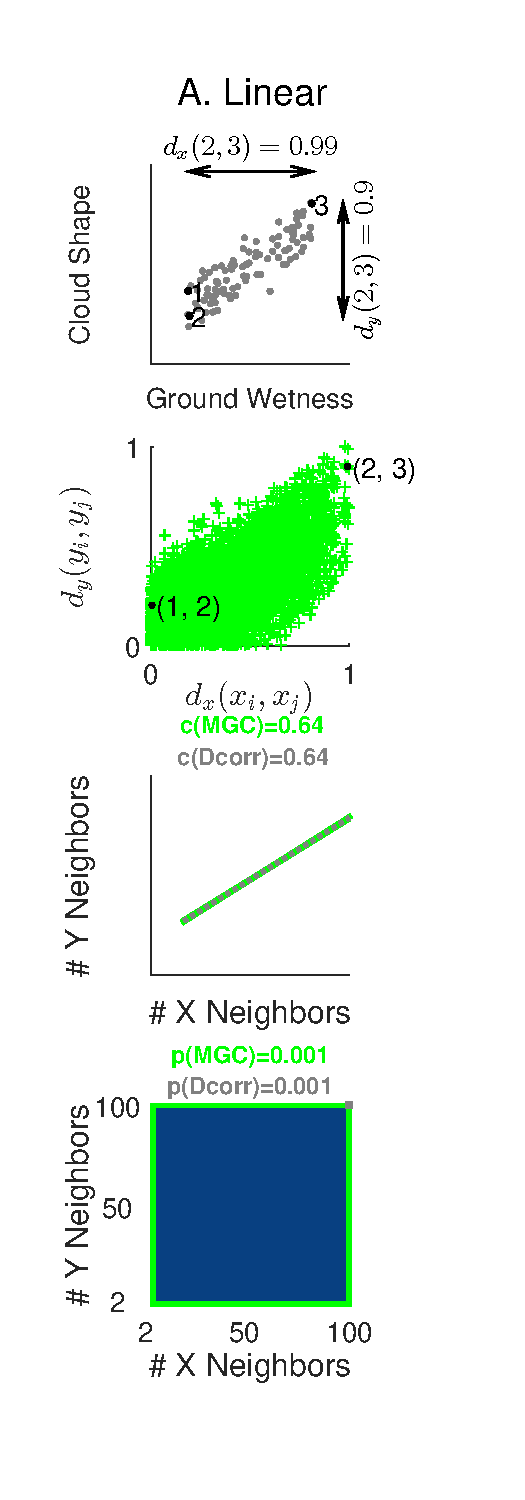
\includegraphics[width=0.32\textwidth,height=0.75\textheight,trim={0.83cm 1.88cm 1.85cm 1.57cm},clip]{Figures/Fig1.pdf}
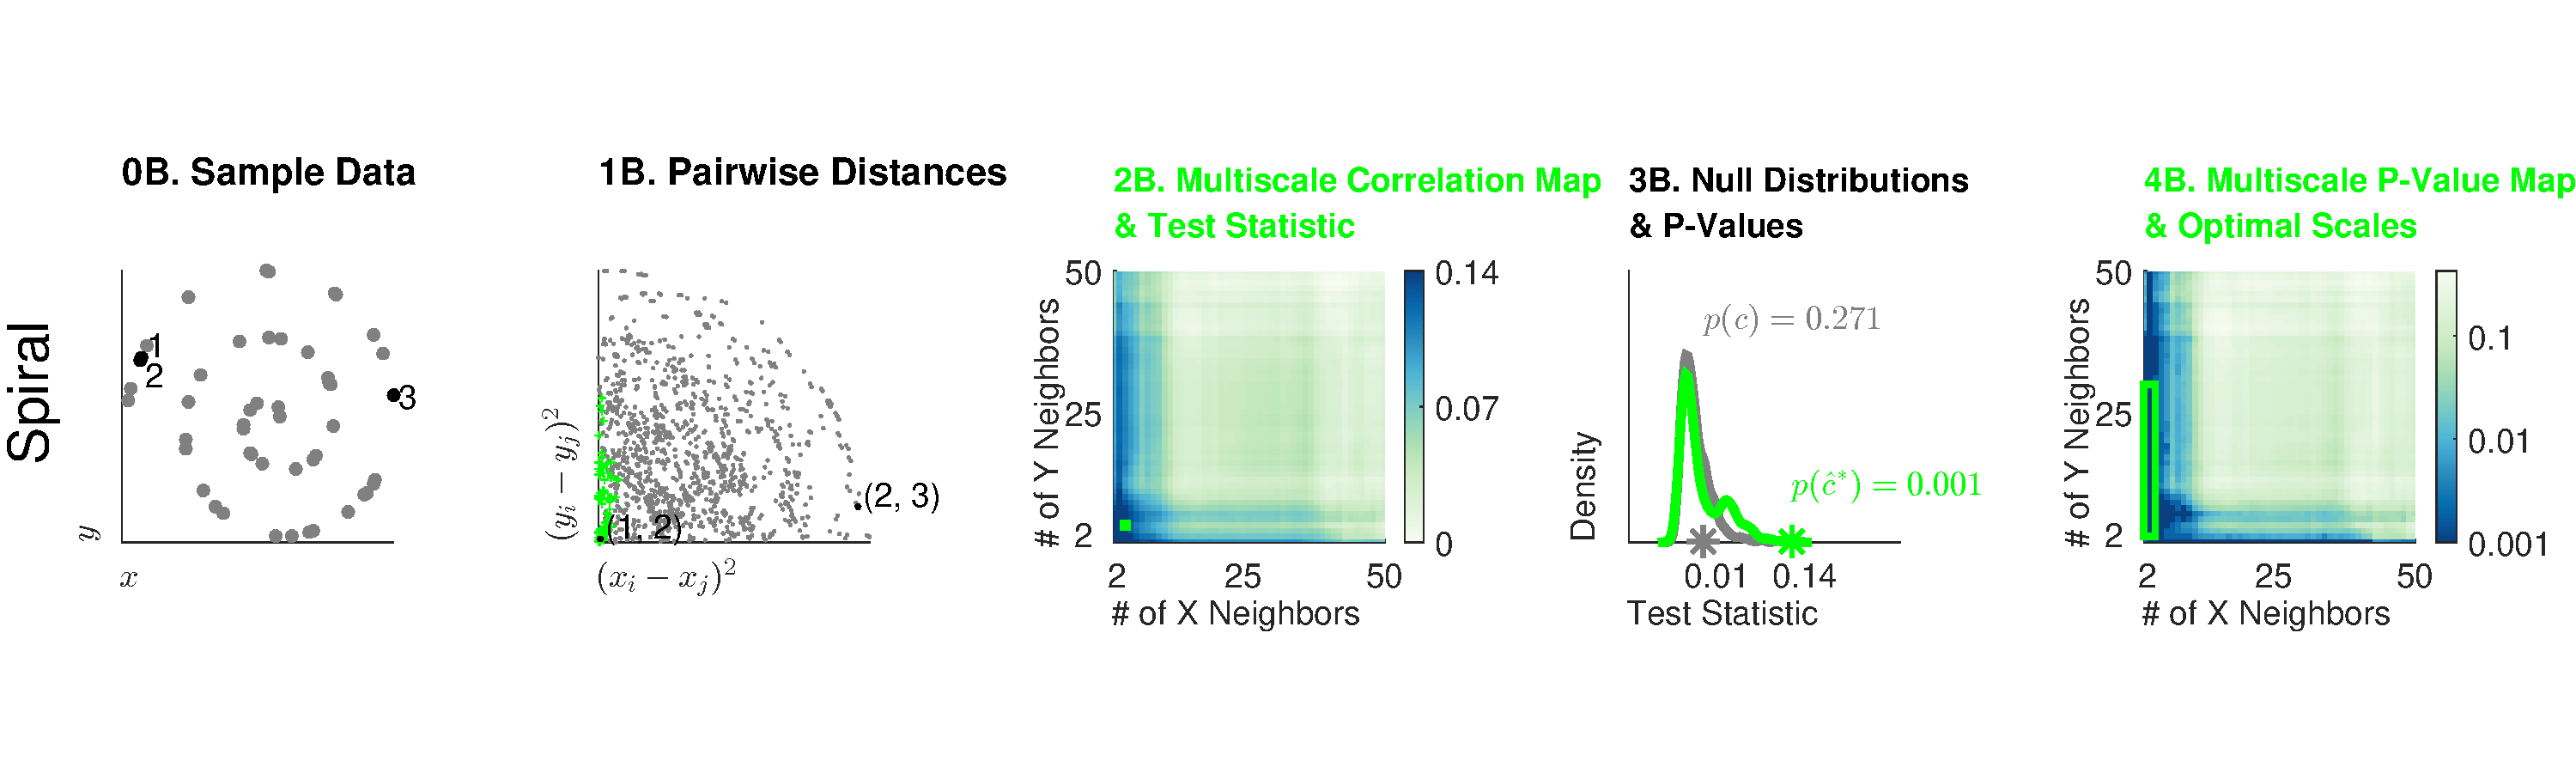
\includegraphics[width=0.32\textwidth,height=0.75\textheight,trim={1.95cm 1.88cm 0.73cm 1.57cm},clip]{Figures/Fig8.pdf}
\caption{Illustration of the three steps of Multiscale Generalized Correlation (\Mgc) in two different settings: linear (center) and nonlinear (spiral; right; see Appendix \ref{appen:function} for simulation details). Insights into the data available only from running \Mgc~are highlighted in green.  Results using \Dcorr, a state of the art dependence test, are shown for comparative purposes. 
\textbf{(0)}  $100$ pairs of samples of cloud density ($x_i$) and grass wetness ($y_i$). 
Samples $1$, $2$, and $3$ (black) indicate how \Mgc~is able to discover nonlinear relationships. 
% 
\textbf{(1)} Distances are linearly correlated in the linear setting, whereas they are not in the spiral setting.  \Dcorr~uses all distances (gray dots) to compute its test statistic, $\GG(\Dcorr)$, which \Dcorr~uses to compute its p-value.
% 
\textbf{(2)} \Mgc~selects a subset of all distances to compute the test statistic (green circles), specifically, only considering the distances within the scales the maximize the local generalized correlation. Title states the maximal local correlation $\GG(\Mgc)$.
% 
\textbf{(3)}
The heatmap shows p-values for all scales (computed via a permutation test), the scale with maximal test statistic after smoothing (green dot), the set of informative scales  (those in the largest rectangle with significant p-values, green box), and the global scale (gray dot). \Mgc~detects significant dependence in both the linear and nonlinear settings, whereas \Dcorr~only detects dependence in the linear setting.% for this small sample size. 
Titles state the p-values,  $p(\Mgc)$~and $p(\Dcorr)$.
% 
\Mgc~is able to detect and reveal the scales of dependence even in highly nonlinear settings with low sample sizes.}
\label{f:newschem}
\end{figure}



Our  dependence test---called ``Multiscale Generalized Correlation'' (\Mgc)---extends essentially all previously proposed pairwise comparison based approaches to enable estimation of the  informative scales.   
Below we demonstrate that \Mgc~can adaptively choose the informative scales for any relationship---linear or nonlinear, high-dimensional or low-dimensional, structured or unstructured---in a computationally efficient and statistically consistent fashion, therefore guaranteeing improved statistical performance over existing global methods for any finite sample size. Moreover, these scales are informative about the nature of the dependence structure, therefore providing further guidance for subsequent experimental or analytical steps. \Mgc~therefore is a hypothesis-testing methodology that builds on recent developments in manifold learning (operating on pairwise comparisons) by combining them with complementary developments in harmonic (multiscale) analysis. 
It is this union of three disparate disciplines spanning data science that enables improved theoretical and empirical performances.  


The first step of \Mgc~is the same as other nonparametric dependency tests such as \Dcorr~\cite{SzekelyRizzo2009} (a celebrated dependence test):
compute the distances between all pairs of cloud densities and the corresponding distances between all pairs of grass wetnesses (Figure \ref{f:newschem}, step 1).
The \Dcorr~test statistic, similar to the other previously proposed global tests, is the correlation of all pairs (see title of step 1 panels).
Only \Mgc~then computes the maximum ``local generalized correlation''.
A local generalized correlation is the correlation only including the $k$ smallest distances for each $x_i$, and the $l$ smallest distances for each  $y_i$.  \Mgc~computes these local generalized correlations for all possible values of $k$ and $l$.
The \Mgc~\emph{test statistic} is the local generalized correlation with the best scale, that is, the $(k,l)$ pair whose generalized correlation is largest after smoothing (\Mgc~smooths to address noisy samples). 
The green circles in Figure \ref{f:newschem}, step 2 show the set of distances that \Mgc~selected for this particular simulation.
For the linear case all the neighbors are used, so  \Mgc's test statistic is the same as \Dcorr's (which uses all neighbors).  For the nonlinear case, however, the set of comparisons is limited to only local pairs, resulting in \Mgc's test statistic being much larger than \Dcorr's test statistic (titles show the maximal test statistics and its' local scale).   

The third and final step is to compute the p-value and the \emph{multiscale significance map}. This map provides the set of informative scales and indicates which scales are maximally informative about the dependence relationship. The p-value for each scale is available from a permutation test.  For each permutation, \Mgc~computes the largest test statistic (after smoothing), which it uses in its test, therefore mitigating any multiple comparison problems. The informative scales are all scales within the largest rectangle with local p-values no larger than the p-value of Sample \Mgc. For the linear example, many scales including the global one (\Dcorr's) yield highly significant p-values, implying a nearly linear relationship.
On the other hand, for the nonlinear setting, only a set of small local scales yields significant p-values, implying a strong nonlinear relationship that \Dcorr~does not detect but \Mgc~reveals.  


Running \Mgc~merely requires inputting $n$ samples of two measured properties.  
% @jovo: explain to brett duality between distances and transformations of the data.
Our open source implementation\footnote{In both MATLAB and R from our website, \website.} requires essentially the same run time as conventional methods, situating it to be useful in a wide variety of contexts. 
% Specifically, computing distances between all pairs of observations---as required by all global methods---requires $\mathcal{O}(n^2)$ time.  By virtue of the above described nested algorithm, the only additional computational overhead for \Mgc~follows from ranking observations, merely a multiplicative factor of $\mc{O}(\log n)$.  Thus, \Mgc~has nearly the same computational complexity of the previously proposed state of the art methods. 
The following sections document \Mgc's empirical, computational, and theoretical properties. Mathematical details of prior global methods are provided in Appendxi \ref{appen:global}, details for \Mgc~are offered in Appendix \ref{appen:mgc}, and \Mgc~pseudocode is provided in Appendix~\ref{appen:algorithms}.



\subsection*{Finite Sample Simulation Experiments}

When does \Mgc~outperform other approaches, and when does it not?
To answer this question, \Mgc~is compared with four previously proposed state of the art tests: \Mantel, which is widely used in biology and ecology despite a lack of theoretical support \cite{Mantel1967}, \Dcorr, as discussed above, \Mcorr, a version of \Dcorr~designed to be unbiased in high-dimensional data \cite{SzekelyRizzo2013a}, and \Hhg, a powerful test designed for low-dimensional nonlinear settings \cite{HellerGorfine2013}. 
Consider $20$ different noisy dependence settings, largely taken from the existing literature, including  nearly linear (1-5), strongly nonlinear (6-19), and independent (20) settings \cite{SzekelyRizzoBakirov2007, SimonTibshirani2012, GorfineHellerHeller2012, HellerGorfine2013, SzekelyRizzo2013a}.  
The function details are shown in Appendix~\ref{appen:function}, with additional supporting figures put in Appendix~\ref{appen:figs} (The visualization of both noise-free (black) and noisy (gray) samples is in Supplementary Figure~\ref{f:dependencies}).  


Each approach is evaluated as a function of increasing the dimensionality of $x$.  Power---the probability of rejecting the null when it is  false---is the standard metric for evaluating test performance of finite samples (see Algorithm~\ref{alg:power} for power computation and Algorithm~\ref{alg:sample_mgc} for \Mgc~test statistic computation).  
For each setting, the power of each test is computed for a large range of different dimensions of $x$,  effectively decreasing the signal-to-noise ratio.  
The average power across dimensions for each algorithm provides a scalar ``score'' per setting.  %Although \Mgc~generalizes essentially any global correlation approach, by default we extend \Mcorr~due to its impressive empirical performance in high-dimensional data.  
Figure~\ref{f:nDSummary} shows the difference between \Mgc's score and the benchmarks for each setting.  
\Mgc~achieves a higher power in essentially all 20 settings when compared to all other approaches.  
Supplementary Figure \ref{f:nDAll} shows the power as a function of dimensionality, rather than the average, which indicates that  \Mgc~almost always achieves higher power than the alternative tests for all dimensions, not just the average dimension.  
 Supplementary Figures \ref{f:1DAll} and \ref{f:1DSummary} show similar results,  but keeping the dimensionality of $x$ fixed while increasing sample size. These supplementary figures also show the performance of different variants of \Mgc~with qualitatively similar results.% in particular, generalizing both \Mantel~and \Dcorr, with qualitatively similar results.



\begin{figure}
  \centering
  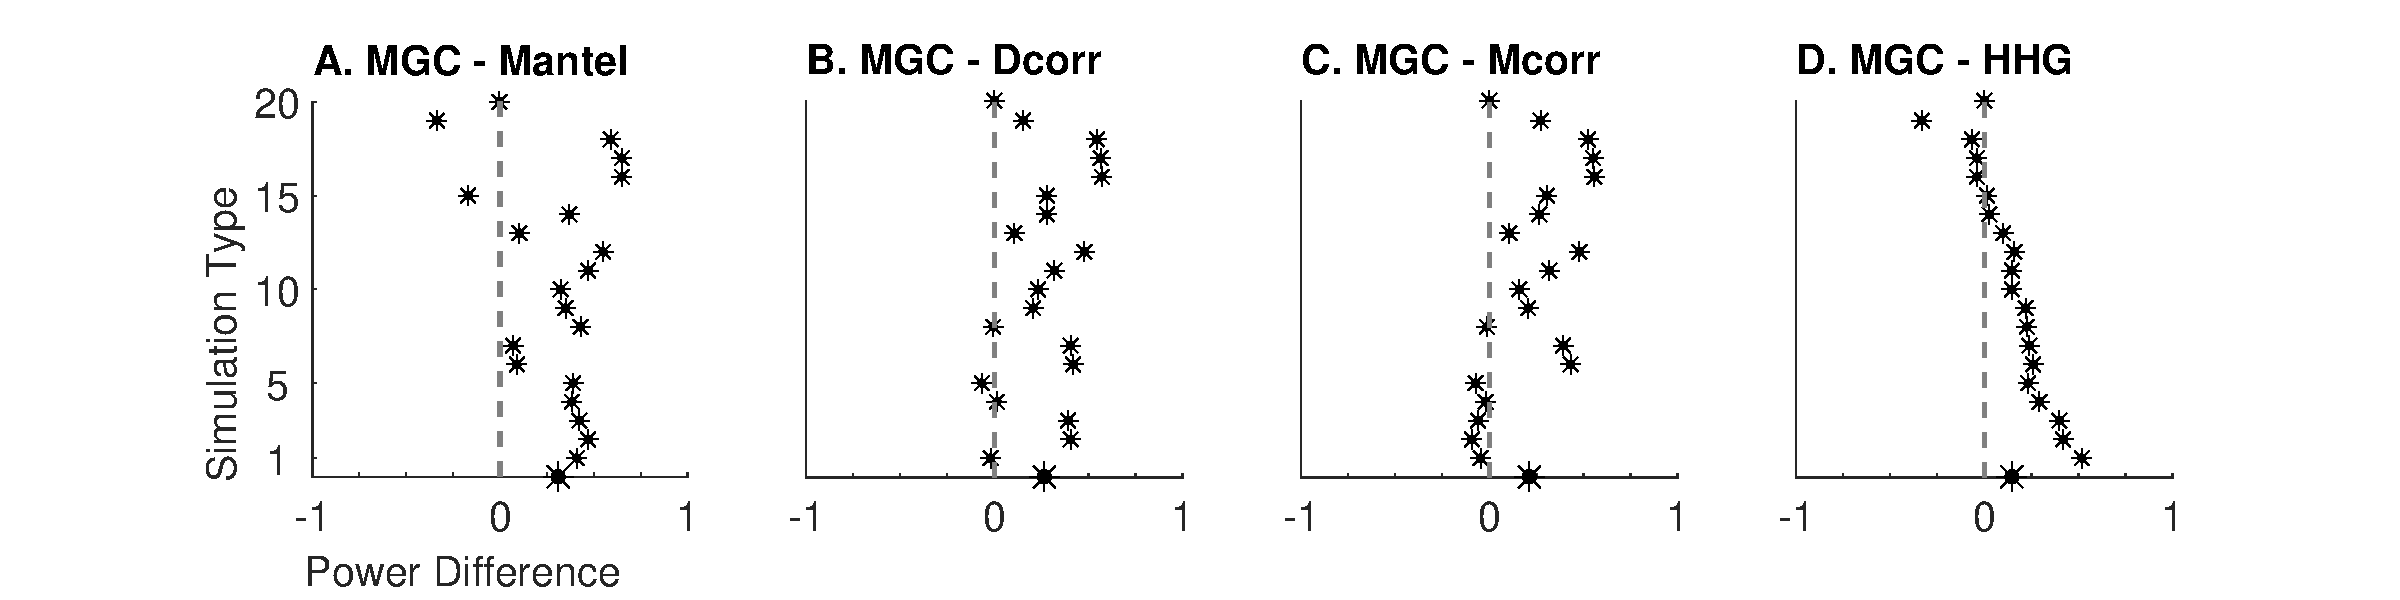
\includegraphics[width=1.0\textwidth,trim={3.5cm 0 3.5cm 0},clip]{Figures/FigHDPowerMGCM}
  \caption{Power comparison of  \Mgc~to four benchmark dependence tests, for the $20$ different settings.  
%   The ``score'', $\bar{\beta}$, for an algorithm and setting is 
Let $\bar{\beta}_p(\mathcal{A})$ denote the average power over a wide range of dimensions for a given problem setting $p$ and algorithm $\mc{A}$. The x-axis shows the difference between the power of \Mgc~and its competitors,  $\bar{\beta}_p(\Mgc)-\bar{\beta}_p(\mathcal{A})$. Power difference $>0$ indicates that \Mgc~achieves higher average power over the benchmark for a given setting;
the large dot on the x-axis indicates the  power differences averaged over all 20 settings.
\Mgc~nearly dominates all benchmarks, exhibiting similar or better power for nearly all settings. 
}
\label{f:nDSummary}
\end{figure}


\subsection*{Discovery of Dependency Across Scales}
\label{main3}

Not only does \Mgc~provides excellent power, but it also reveals the informative scales of dependence. 
A \emph{multiscale power map} is a heatmap that shows, for a given simulation, the power as a function of the $x$ and $y$ scales.  
Figure~\ref{f:powermaps} provides the multiscale power maps for all 20 different high-dimensional scenarios, illustrating how the power of local correlations changes with  neighborhood size.
For nearly linear dependencies (1-5), the best neighborhood choice always includes the largest scale, i.e., the global one. For all strongly nonlinear dependencies (6-19),  \Mgc~chooses smaller scales for $x$ or $y$. Thus, a global optimal scale implies a nearly linear dependency, otherwise the dependency is strongly nonlinear.
Furthermore, similar dependencies have similar local correlation structure, and thus, similar informative scales. For example, (10) and (11), though very different functions analytically, are qualitatively similar, and yield very similar multiscale power maps.
Similarly,  (12) and (13) are trigonometric functions, and they share a narrow range of significant local correlations.
Both circle (16) and ellipse (17), as well as square (14) and diamond (18), are closely related functions, and have similar multiscale power maps. 

For real data that power is unavailable (because the true distribution is unavailable), \Mgc~provides a multiscale p-value map (see Algorithm~\ref{alg:pval}) that is a noisy version of the power map, as well as the multiscale correlation map (see Algorithms~\ref{alg:1scale} and~\ref{alg:all_scales}), based on which the informative scales are estimated. The green dot and rectangle in each panel of Figure~\ref{f:powermaps} correspond to the estimated test statistic and informative scales by \Mgc~on one pair of sample data without knowing the underlying distribution. The estimations are often very close to true optimal choices based on the actual power maps when knowing the model.

\begin{figure}[htbp]
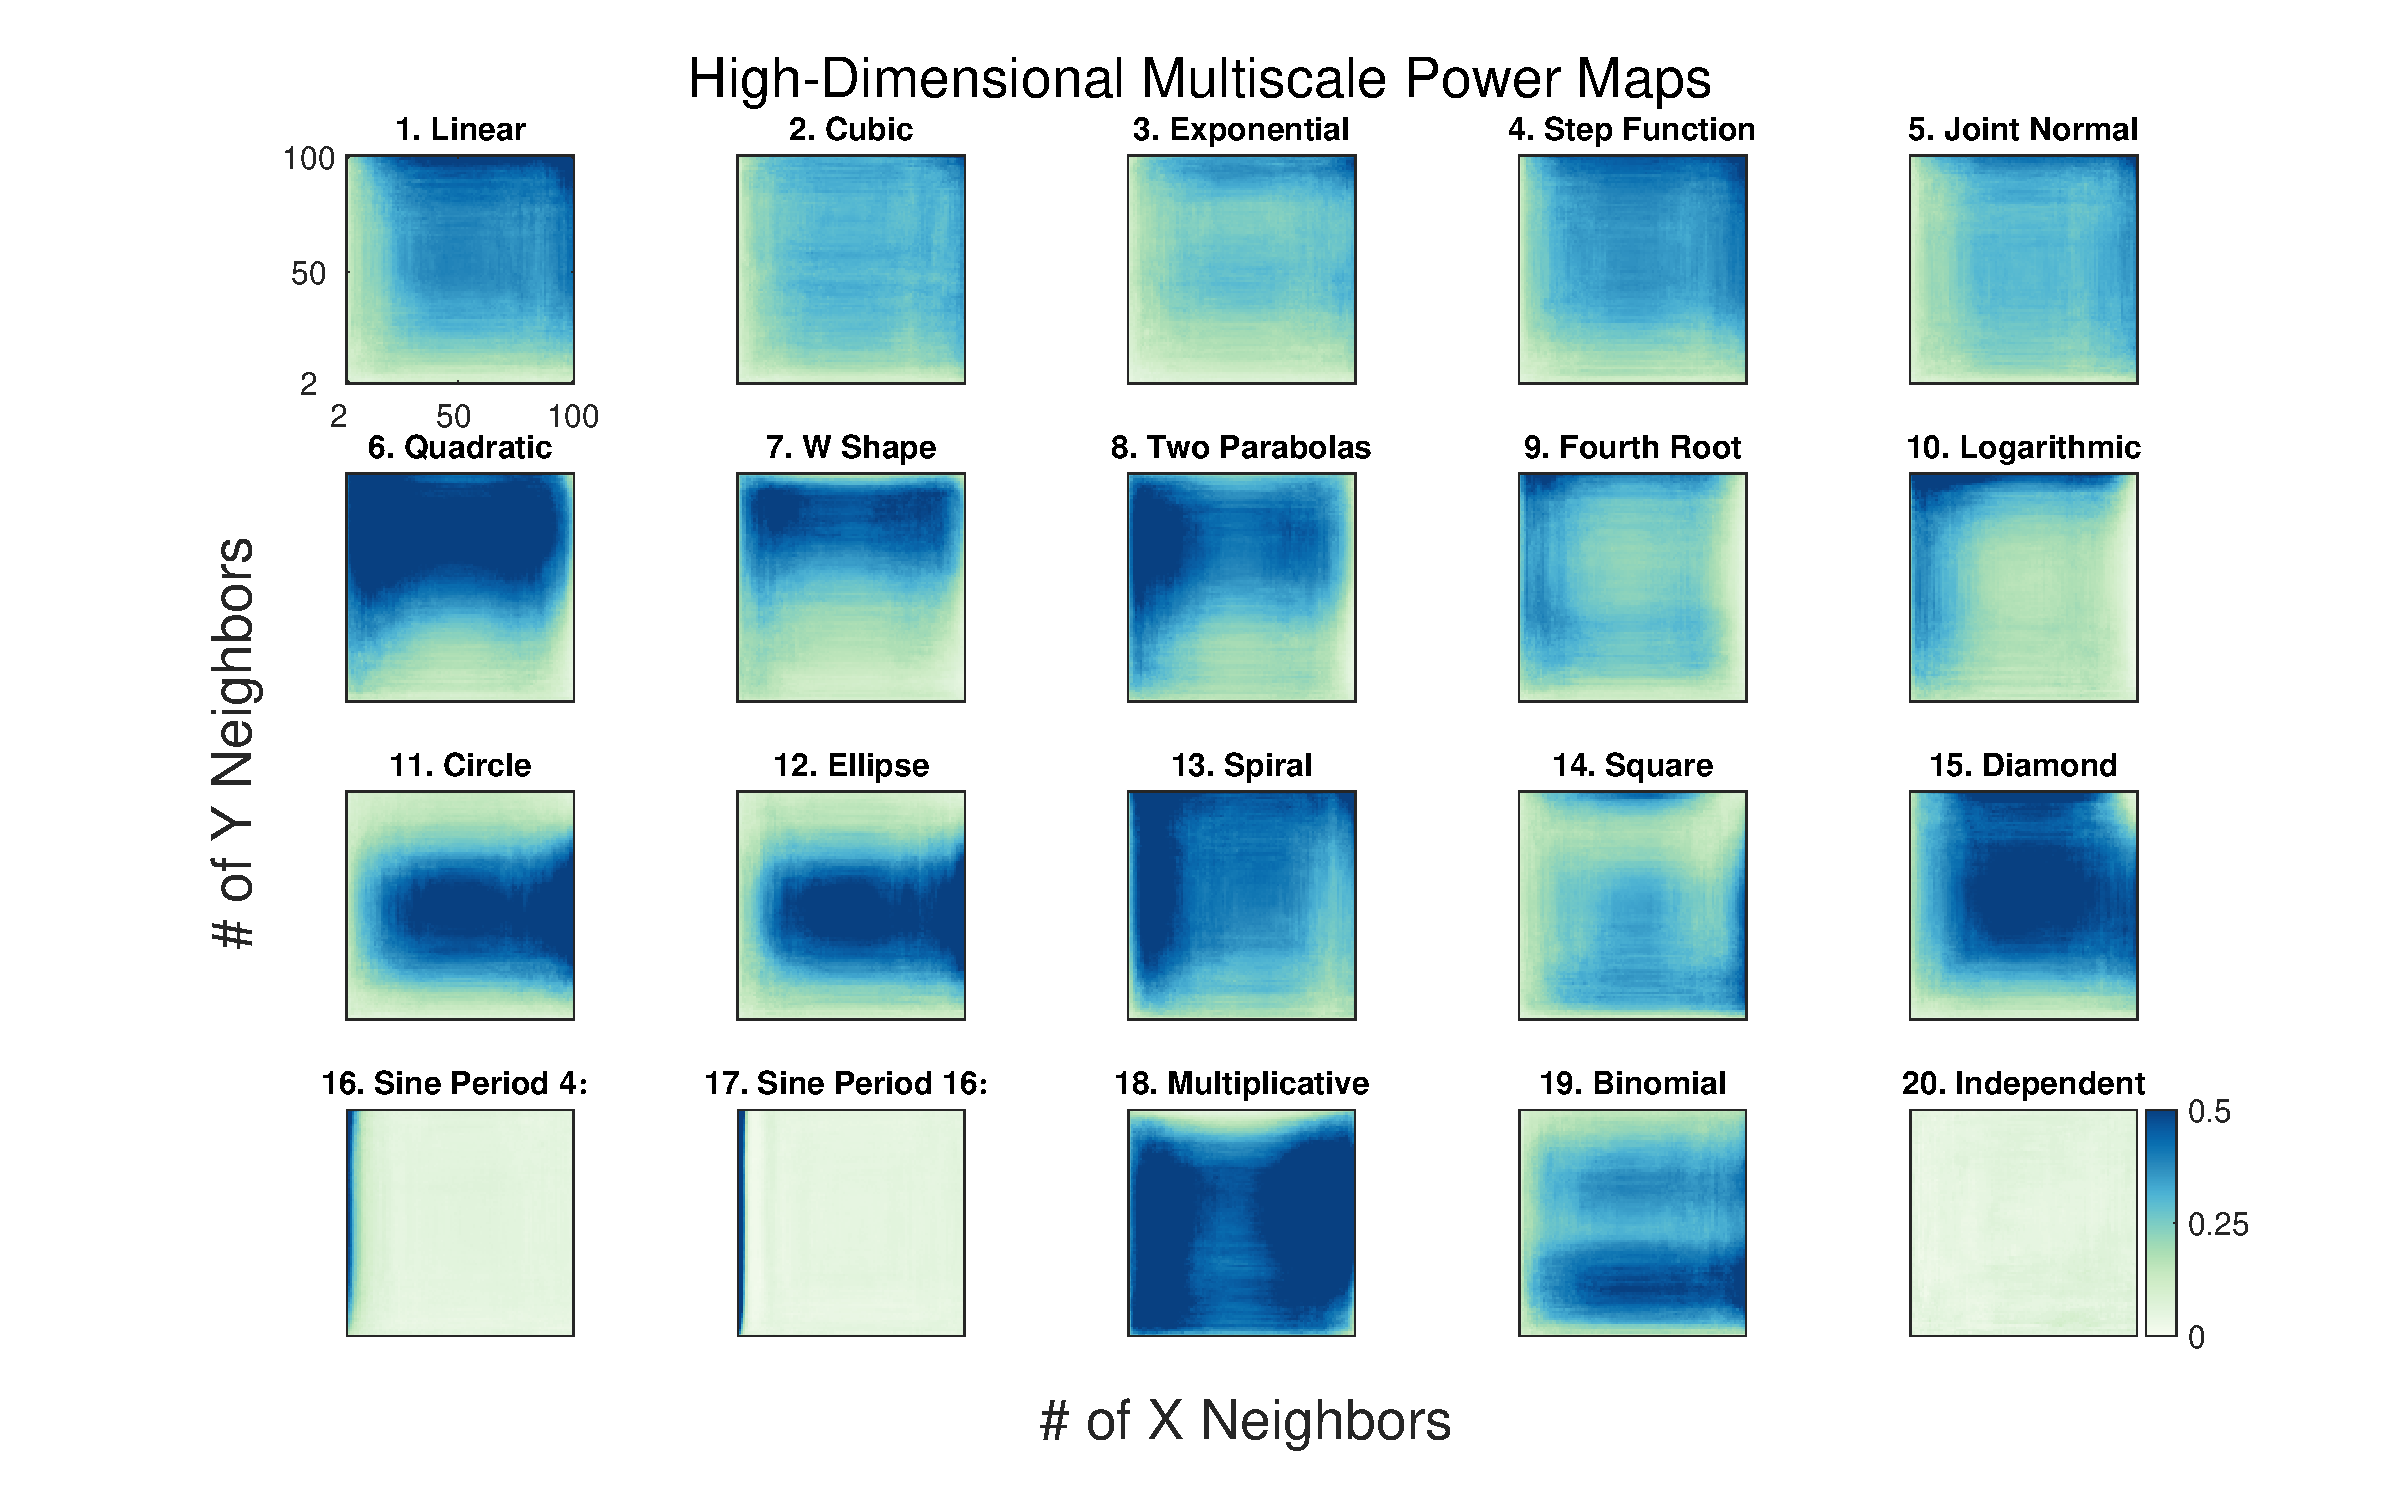
\includegraphics[width=1.0\textwidth,trim={3cm 0.5cm 2.5cm 0.5cm},clip]{Figures/FigHDHeat}
\caption{Multiscale Power Maps reveal the influence of neighborhood size on \Mgc~testing power.
For each of the 20 panels, the abscissa and ordinate denote the number of neighbors for $X$ and  $Y$, respectively, and the color denotes the power at that scale. For each simulation, the sample size is $100$,  and the dimension is determined by the largest dimension for \Mgc~to have power exceeding $0.5$ at significance level $0.05$. Each simulation yields a different multiscale power map, and the global scale is optimal only for nearly linear dependencies, highlighting that \Mgc~not only detects the mere existence of dependency, but also reveals its  structure. 
For each panel, the green dot and rectangle show the estimated test statistic and the estimated informative scales via \Mgc~on one pair of sample data without knowing the underlying distribution, which are often close to optimal choices of the power map.
}
\label{f:powermaps}
\end{figure}


\subsection*{\Mgc~Theoretically Dominates its Global Counterparts}
\label{s:theory}

``Oracle \Mgc'' is a version of \Mgc~that uses the true distribution of the data to accurately select the optimal local correlation, rather than estimating it from the data (see section~\ref{appen:mgc2} for details). More specifically, Oracle \Mgc~selects the scale that maximizes power, whereas ``Sample'' \Mgc~selects the scale that maximizes the smoothed test statistic. 
In either case,  \Mgc~can generalize any distance based dependence test by restricting it to only consider local distances.  Any global test that \Mgc~generalizes is called \Mgc's ``global counterpart''.  The main theoretical result we obtain is as follows:
% 
\begin{thm} \label{t:dominate}
Oracle \Mgc~statistically dominates its global counterparts. Thus, no matter which global correlation is generalized, dependence function, dimensionality, and sample size, Oracle \Mgc~achieves equal or higher power than its global counterparts.  More precisely, in \emph{linear} settings Oracle \Mgc~achieves the same power as the global test, and in various nonlinear settings, Oracle \Mgc~achieves {higher} power than the global test. Moreover, Algorithm \ref{alg:all_scales} achieves this dominance with merely an additional multiplicative computational cost of $\log n$, rather than an additional $n^2$ that would result from a na\"ive implementation.
\end{thm}

The above result follows immediately from Theorems \ref{t:thm1}, \ref{t:linear}, and \ref{t:non}, which are described in Appendix \ref{appen:theory}.   Empirically, Sample \Mgc~performs very closely to Oracle \Mgc~in most simulated settings (see Supplementary Figure \ref{f:nDAll} and \ref{f:1DAll}), suggesting that Sample \Mgc~may also dominate global methods with high probability.

\subsection*{Real Data Experiments}
\label{numer3}

\Mgc~can be applied to real data scenarios with complex structure, provided appropriate distance measures are available. We apply \Mgc~to three different scenarios: (i) brain activity versus personality, (ii) brain shape versus disease, and (iii) brain networks versus creativity.  These three brain properties span the most popular \emph{in vivo} whole brain techniques and representations of the brain: functional, structural, and diffusion magnetic resonance imaging; while the different mental properties span cognition and health.  For each comparison, we chose appropriate distances for both kinds of data, and ran \Mgc~to obtain both a p-value and a multiscale significance map, akin to the multiscale power maps shown above, but for real data for which power is unavailable. \Mgc~reveals a statistically significant relationship for all three, and is the only approach that also provides insight into the nature of the relationship. 
This deeper insight provides guidance for the subsequent analysis tasks, including predictions and causal analysis. As a final test for \Mgc, synthetic data for which no relationship exists are generated, and \Mgc~does not yield spurious relationships, in contrast to popular parametric methods \cite{EklundKnutsson2012,Eklund2015}. 


\subsubsection*{Brain Activity vs. Personality} 

This experiment investigates whether there is any dependency between brain activity and personality.
Adelstein et al. \cite{AdelsteinEtAl2011} were able to detect dependence between certain regions and dimensions of personality, but lacked the tools to test for dependence of the whole brain activity against all five dimensions of personality. 
This dataset consists of $n=42$ subjects, each with  $197$ time-steps of resting-state functional MRI activity, as well as the subject's five-factor personality trait as quantified by  the NEO Personality Inventory-Revised  \cite{Costa1992}. 
For the brain activity modality, we derived the following comparison function. For each scan, (i) 
run the Configurable Pipeline for the Analysis of Connectomes (C-PAC) pipeline \cite{CPAC2015} to process the raw brain images yielding a parcellation into $197$ regions of interest, 
(ii) run a spectral analysis on each region, (iii) bandpass and normalize it to sum to one, and (iv) calculate the Kullback-Leibler divergence across regions to obtain a similarity matrix across comparing all regions.  Then, use the normalized Hellinger distance to compute distances between each subject. 
For the five-factor personality modality, we  used the Euclidean distance.
% 
Figure \ref{f:real}{\color{magenta}A}  shows that many local scales yield significant p-values ($\approx 0.01$), whereas the global scale fails to detect this significant dependence. In fact, all previously proposed global dependence tests under consideration (\Mantel, \Dcorr, \Mcorr, or \Hhg) fail to detect dependence at a significance level of $0.05$ (see Table \ref{t:real}), and only \Mgc~provides insight into the scales of dependence.

\subsubsection*{Brain Shape vs. Disease} 


The next experiment investigates whether brain shape and disease status are dependent on one another.  Previous investigations have linked major depressive disorder to the hippocampus shape \cite{ParkEtAl2008,PosenerEtAl2003}, though global tests were unable to detect a statistically significant dependence structure at the $\alpha=0.05$ level.
This brain shape versus disease dataset consists of $n=114$ subjects. Each subject has a structural MRI scan as well as a discrete variable indicating whether the subject is non-affected $(0)$, high-risk $(1)$, or clinically depressed $(2)$.  From the MRI data, previous work extracted both the left and right hippocampi. For the brain shape modality, comparison matrices using a nonlinear landmark matching approach were generated \cite{ParkEtAl2008,BegEtAl2005}. For the disorder variable, we added white noise bounded by $0.01$ to each label, then formed the Euclidean distance (the noise is used to break ties amongst the discrete values and make sure only the diagonal entries of the distance matrix are zero).
% 
Figure \ref{f:real}{\color{magenta}B} provides the p-value map for testing on the right hemisphere using \Mgc. Again, many local scales yield significant p-values, whereas none of the global methods detect a significant dependence  (see Table \ref{t:real}). 

\begin{figure}[htbp]
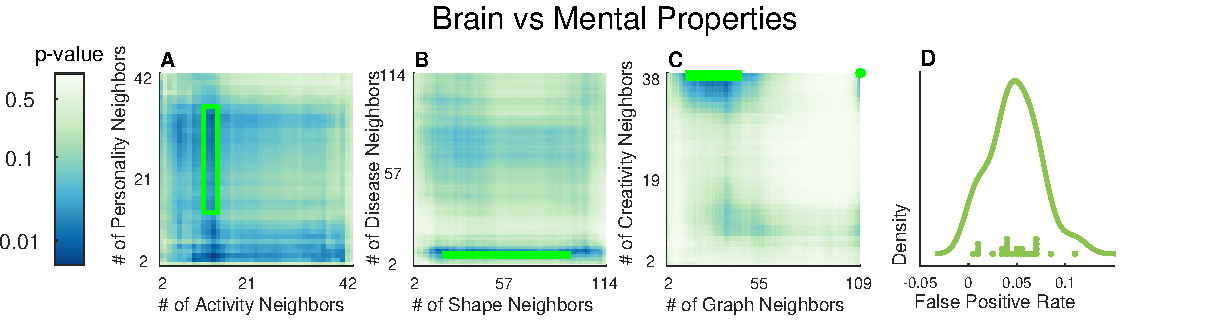
\includegraphics[width=1.0\textwidth,trim={0 0 1.5cm 0},clip]{Figures/FigReal}
\caption{In real data, \Mgc~discovers the dependence and informative scales between various brain and mental properties when they exist, and does not detect dependence when it does not exist.  The left three panels show multiscale p-value maps and their corresponding informative scales for three different experiments: \textbf{(A)}  brain activity vs. five-factor personality model, \textbf{(B)}  brain shape vs depressive disease, and \textbf{(C)} brain networks vs. creativity. Sample size is $42$, $114$, and $109$, respectively, though the ordinate of these panels only goes as high as the largest possible neighborhood size due to repeated entries.  
For all three, \Mgc~yields a significant p-value and reveals the informative scales of dependence (green rectangles).
\textbf{D.} Density estimate for the false positive rates of  \Mgc~on the brain activity versus synthetic independent noise experiments, dots indicate with the false positive rate of each experiment. The mean $\pm$ standard deviation is $0.0538 \pm 0.0394$ respectively, demonstrating that \Mgc~is a valid test and does not inflate the false positives for these real data.}
\label{f:real}
\end{figure}

\begin{table*}[htbp]
\centering
\caption{The p-values for real data testing. \Mgc~is the only method that \emph{always} uncovers the existence of significant relationships and the only method that \emph{ever} discovers the underlying informative scales. Bold indicates lowest p-value per dataset.}
\label{t:real}%
\begin{tabular}{|c||c|c|c|c|c|}
\hline
Testing Pairs / Methods & Sample \Mgc & \Mantel & \Dcorr & \Mcorr & \Hhg \\
\hline
Activity vs Personality & $\textbf{0.033}$  & $0.988$ & $0.647$ & $0.446$ & $0.056$ \\
\hline
Shape vs Disease & $\textbf{0.019}$  & $0.079$ & $0.108$ & $0.106$ & $0.179$ \\
\hline
Network vs Creativity & $\textbf{0.011}$  & ${0.012}$ & $\textbf{0.011}$ & $\textbf{0.011}$ & ${0.033}$ \\
\hline
\end{tabular}
\end{table*}

\subsubsection*{Brain Network vs. Creativity}

The next experiment investigates whether brain structural networks are independent of creativity.  Neural correlates of creativity have previously been investigated, though largely using structural MRI and cortical thickness \cite{Jung2009}.  Previously published results demonstrated graph similarity between subjects with similar creativity \cite{Koutra15a}. Those data include  $n=109$ subjects, each with diffusion weighted MRI (dMRI) data as well as the subject's ``creativity composite index'' (CCI).  
For the raw brain imaging data, we derived the following comparison function.  For each scan, (i) process diffusion and structural MRI data via  \Migraine, a pipeline for estimating brain networks from diffusion data \cite{GrayRoncal2013}, (ii) 
compute the distance between brain networks using the semi-parametric graph test statistic \cite{Sussman2013,ShenVogelsteinPriebe2016,Tang2016}, embedding each graph into two dimensions for simplicity and aligning the embeddings via a Procrustes analysis.  Then, compute the Euclidean distance between subjects. We used Euclidean distance to compare CCI values. 
% 
Figure \ref{f:real}{\color{magenta}C} shows that even global dependence tests can ascertain whether the whole brain network is independent of the subject's creativity.  \Mgc~demonstrates that the signal in this case is largely captured by a global relationship, suggesting that there is relatively little to gain by pursuing nonlinear regression techniques. In this setting with high-dimensional and structured data samples and low-sample size, \Mgc~can reveal a strongly linear dependence (lacking a strong nonlinear dependence) without having to resort to structured regression techniques.


\subsubsection*{\Mgc~Does Not Inflate False Positive Rates} 


In the final experiment, \Mgc~is applied to test independence between brain voxel activities and a non-existent stimulus, similar to a pair of studies led by Eklund  \cite{EklundKnutsson2012,Eklund2015}. We considered $25$ resting state fMRI data sets from the $1$,$000$ functional connectomes project (\url{http://fcon_1000.projects.nitrc.org/}), consisting of a total of $1$,$583$ subjects.
Then an independent stimulus are generated by sampling from a standard normal distribution at each time step. The brain activity data and the stimuli are independent by construction.
For each brain region, \Mgc~attempts to address the following question: Is activity of that  brain region independent of the time-varying stimuli? We pool brain activity over all of the samples from the population.
Any region that is detected as significant is a false positive by definition.  By testing each brain region separately, \Mgc~provides a distribution of false positive rates.  If \Mgc~is valid, that distribution should be centered around the significance level, which is set at $0.05$ for this experiment.

Conducting \Mgc~requires a distance matrix for brain region activity, and another for the stimulus. For the brain region activity, we used C-PAC to estimate regional time-series, in particular, using the sequence of pre-processing decisions determined to optimize discriminability \cite{Wang2016}.  The output for each scan is the resting state fMRI time series data containing $200$ regions of interest for $200$ time-steps.
For each region, the Euclidean distance pairs between time steps are computed, i.e., $\|\mb{x}_{\cdot i}-\mb{x}_{\cdot j}\|_2$,  where $\mb{x}_{\cdot i}$ denotes the population vector of activity of the region at time-step $i$ for all subjects.
For the one-dimensional stimulus, we similarly compute the Euclidean distance between the stimulus values at each pair of time-steps: $\|\mb{y}_i - \mb{y}_j\|_2$.
Note that the distance matrices at different brain regions are distinct, but the stimulus is the same for all brain regions during the same experiment.


For each data set, the above test is carried out for each brain region. 
Figure~\ref{f:real}{\color{magenta}D} shows the false positive rates of  \Mgc~for each dataset, which are centered around the critical level $0.05$, as it should be.
In contrast, many standard parametric methods for fMRI analysis, such as generalized linear models, can significantly increase the false positive rates, depending on the data and pre-processing details \cite{EklundKnutsson2012,Eklund2015}. Moreover, even the proposed solutions to those issues make linearity assumptions, thereby limiting detection to only a small subset of possible dependence functions.

\subsection*{Discussion}
\label{conclu}

We propose multiscale generalized correlation (\Mgc) to discover the presence and scales of dependence across disparate types of data.
We proved that Oracle \Mgc~dominates global approaches in finite samples.  This proof shows that \Mgc~performs as well as global approaches in certain settings (the linear ones), and better than global approaches in other settings (nonlinear ones). 
We further empirically demonstrate, via simulations, that \Mgc~outperforms global methods regardless of the dimension, sample size, or nonlinearity.  Moreover, \Mgc~provides a map indicating which scales contain the dependence structure. 
In real data experiments, \Mgc~reveals dependence where global methods fail, as well as the nature of those dependencies, and does not falsely detect signals when there are none.

Several other approaches to dependence detection deserve further mention. First, kernel-based independence tests  \cite{GrettonEtAl2005, GrettonGyorfi2010, GrettonEtAl2012} are equivalent ``energy statistics'' (such as \Dcorr~and \Mcorr) \cite{SejdinovicEtAl2013, RamdasEtAl2015}. Thus, we may be able to glean further insights by casting \Mgc~within the kernel framework, or applying \Mgc~to those tests. Specifically, more efficient tests using asymptotic null distribution approximations for our multiscale tests are possible.
Second, Reshef et al. \cite{Reshef2011} and Heller et al. \cite{heller2016consistent} have a different starting configuration, and are therefore slightly more difficult to generalize than the energy statistics based tests.  Nonetheless, they can perform well especially in some $1$-dimensional settings \cite{SimonTibshirani2012, reshef2015empirical}, so further investigation seems worthwhile. 


 \Mgc~can be thought of as a regularized, or sparsified variant of generalized correlation coefficients.  Regularization is central to high-dimensional and ill-posed problems, where dimensionality is larger than sample size. The connection made here between regularization and dependence testing opens the door towards considering other regularization techniques for correlation based dependence testing. For example, \Hhg~can be thought of as averaging over all scales, rather than regularizing to only consider the optimal ones. The Reshef approach can be thought of similarly.  Therefore, we suspect that the ideas underlying \Mgc~could be implemented in other statistical testing frameworks.


There are a number of additional potential extensions of this work. First, theoretical guidance for choosing the optimal scale for finite samples in the absence of training data is desirable. 
In this work, we proved that there exist optimal local scales that improve upon the global scale, and demonstrated that Sample \Mgc~yields tests with power very close to the optimal power, often better than \Hhg~and \Mcorr, and with significant p-values and accurate optimal scale estimation in the real data examples. More theory connecting Oracle \Mgc~and  Sample \Mgc~will yield further insight.

Second, \Mgc~requires a pair of metrics (or distances), one for each data type. In this work we selected such metrics using domain knowledge, and mitigated the potential inopportune choice of metric via locality tuning.  If the optimal metric could be reasonably selected for a given dataset, this would possibly obviate the need for locality, and further improve power. Szekely et al. investigated different norms and exponents to ascertain the impact of different metrics, but was unable to determine optimality.
Metric learning \cite{xing2003distance} addresses learning metrics for different exploitation tasks, so perhaps could inform solution to this problem.
In fact, \Mgc~can be thought of as a two-dimensional family of ``metrics'', from which the optimal one is determined in a data adaptive fashion.  Perhaps a different low-dimensional family of metrics could further optimize metric and scale.

Third, essentially all of the tests described in this manuscript are quadratic in sample size.  When sample size gets very large, computational burden becomes intractable. Huo and Szekely  recently developed efficient algorithms that are linear in sample size for one-dimensional data \cite{Huo2016}.  Although it is not clear how to extend the Huo and Szekely approach to multidimensional data, a subsampling strategy seems viable. In fact, ongoing work suggests the multiscale power maps are accurate even when subsampling the data points significantly, suggesting that subsampling data or pairwise comparisons could yield an approximate linear time algorithm without sacrificing the testing power.  One could also implement \Mgc~using a semi-external memory and NUMA architecture computing model \cite{Zheng2016},  which could enable use of solid state disk space in a streaming fashion to both speed up computations for big data and enable storing interpoint pairwise comparison matrices larger than main memory.

Finally, the notion of multiscale generalized correlations could be used in a wide variety of related exploitation tasks.  In particular, energy statistics---for which $\Dcorr$ and $\Mcorr$ are special cases---have been applied to many different testing scenarios, including goodness-of-fit  \cite{Szekely2005}, analysis of variance  \cite{Rizzo2010}, conditional dependence  \cite{Szekely2014,Wang2015},   and feature selection \cite{LiZhongZhu2012,Zhong2015}.     
In fact, \Mgc~can also implement a two-sample (or generally the $K$-sample) test \cite{Szekely2004, heller2016consistent}, and further comparisons of \Mgc~to standard methods for two-sample testing could be illuminating.
Testing independence between graphs and node attributes \cite{Fosdick2015} is another immediate potential application.  And use of the \Mgc~intuition for dimensionality reduction, classification, and regression seems promising.

% jovo: something about other things, like isomap, LLE, etc....


\clearpage
\pagestyle{empty}
\bibliographystyle{Science}
\bibliography{MGCbib}


\section*{Acknowledgment}
% \addcontentsline{toc}{section}{Acknowledgment}
This work was partially supported by the
%
National Security Science and Engineering Faculty Fellowship (NSSEFF),
%
the Johns Hopkins University Human Language Technology Center of Excellence (JHU HLT COE),  the
%
Defense Advanced Research Projects Agency's (DARPA) SIMPLEX program through SPAWAR contract N66001-15-C-4041,
%
the XDATA program of DARPA administered through Air Force Research Laboratory contract FA8750-12-2-0303,
%
the Office of Naval Research contract N00014-12-1-0601,
%
the Air Force Office of Scientific Research contract FA955014-1-0033. The authors thank Dr. Brett Mensh of Optimize Science for acting as our intellectual consigliere, and Dr. Ruth Heller and Dr. Yakir Reshef for insightful suggestions.


\clearpage
\appendix
\setcounter{figure}{0}
\renewcommand{\thealgorithm}{C\arabic{algorithm}}
\renewcommand{\thefigure}{E\arabic{figure}}
\renewcommand{\thesubsection}{\thesection.\Roman{subsection}}
%\renewcommand{\thesubsubsection}{\thesubsection.\Roman{subsubsection}}

\section{Global Methods for Testing Dependence}
\label{appen:global}
To better understand the multiscale generalized correlation, in this section we first formally state the testing scenario, followed by introducing the notion of the generalized correlation coefficient and reviewing four existing dependence tests: the \Mantel~test, distance correlation (\Dcorr), modified distance correlation (\Mcorr), and \Hhg. They are arguable the most popular and well-known statistical tests for dependence, and serve as the benchmarks in this paper. Note that the first three are conventional correlation measures, which can be used for building up local correlations and thus  \Mgc.

\subsection{Testing Independence}

To theoretically investigate the performance of any dependence test requires formalizing the statistical hypotheses.
 Given pairs of observations $(\mb{x}_{i},\mb{y}_{i}) \in \Real^{D \times D_y}$ for $i=1,\ldots,n$, assume they are independently identically distributed as $(\mbx,\mby) \iid f_{xy}$. If the two random variables \mbx~and \mby~are independent, the joint distribution equals the product of the marginals, i.e., $f_{xy}=f_x f_y$.  The statistical hypotheses for testing independence is as follows:
\begin{align*}
& H_{0}: f_{xy}=f_{x}f_{y},\\
& H_{A}: f_{xy} \neq f_{x}f_{y}.
\end{align*}
Given a test statistic, the testing power equals the probability of rejecting the independence hypothesis when the null hypothesis is false. A test statistic is consistent if and only if the testing power increases to $1$ as sample size increases to infinity. We would like a test to be consistent against most (if not all) dependencies, e.g., \Dcorr, \Mcorr, and \Hhg~are consistent against all dependencies with finite second moments. % which is almost as good as universal consistent in practice because real data are always bounded.

Note that $D$ is the dimension for $\mb{x}$'s, $D_y$ is the dimensionality for $\mb{y}$'s. For \Mgc~and all benchmark methods, there is no restriction on the dimensions, i.e., the dimensions can be arbitrarily large, and $D$ is not required to equal $D_y$. The ability to handle data of arbitrary dimension is crucial for modern big data, and it is important to recognize tests that excel for high-dimensional data. There also exist some special methods that only operate on 1-dimensional data, such as \cite{Reshef2011,heller2016consistent,Huo2016}, which are not yet generalize-able to multidimensional data and thus not considered in this paper.

\subsection{Generalized Correlation}
Instead of relying on the the sample observations directly, most state-of-art dependence tests operate on pairwise comparisons, either similarities (such as kernels) or dissimilarities (such as distances). 
Given pairs of observations $(\mb{x}_{i},\mb{y}_{i}) \in \Real^{D \times D_y}$ for $i=1,\ldots,n$, let $\delta_x$ be the distance function for $\mb{x}$'s and $\delta_y$ for $\mb{y}$'s, one can compute two $n \times n$ distance matrices $\tilde{A}=\{\tilde{a}_{ij}\}$ and $\tilde{B}=\{\tilde{b}_{ij}\}$, where $\tilde{a}_{ij}=\delta_x(\mb{x}_i,\mb{x}_j)$ and $\tilde{b}_{ij}=\delta_y(\mb{y}_i,\mb{y}_j)$. A common example of the distance function is the Euclidean metric (or $L^{2}$ norm), which serves as the starting point for all methods in this manuscript.

Assuming two zero-mean matrices $A$ and $B$ are transformations of $\tilde{A}$ and $\tilde{B}$ (e.g., $A$ and $B$ can be the centered distance matrices),
then a ``generalized correlation coefficient''  \cite{Spearman1904,KendallBook} is written as:
\begin{equation}
\label{generalCoef}
\GG(X,Y)= \tfrac{1}{z} {\textstyle \sum_{i,j=1}^n a_{ij} b_{ij}},
\end{equation}
where $z$ is proportional to the standard deviations of $A$ and $B$, that is $z=n^2\sigma_a \sigma_b$, and $X=\{\mb{x}_{1},\cdots, \mb{x}_{n}\} \in \Real^{D \times n}$ and $Y=\{\mb{y}_{1},\cdots, \mb{y}_{n}\} \in \Real^{D_y \times n}$ denote the matrices of sample observations.

In words, $\GG$ is the global correlation across \emph{pairwise comparison matrices} $A$ and $B$, rather than the individual data samples. By defining $A$ and $B$ based on different transformations of 
the distance matrices, the \Mantel~coefficient, \Dcorr, and \Mcorr~can all be written in the form of the generalized correlation coefficient. Note that traditional correlations such as the Pearson's correlation and the rank correlation can also be written by a generalized correlation coefficient, where $A$ and $B$ are derived from sample observations rather than distances; and the \Hhg~test  cannot easily be cast into this framework even though it is operating on distances.

A generalized correlation always ranges in $[-1,1]$, has expectation $0$ under independence, implies a stronger dependency when the correlation is further away from $0$, and can serve as the global correlation in implementing \Mgc. 

To carry out the hypothesis testing on sample data by a given test statistic, e.g., a generalized correlation, the permutation test is the usual choice \cite{GoodPermutationBook}, because a p-value can be computed by comparing the correlation of the sample data to the correlation of the permuted sample data. The independence hypothesis is rejected if the p-value is lower than a pre-set type $1$ error level, say $0.05$. Then the testing power of the generalized correlation equals the probability of correct rejection.

\subsubsection{The \Mantel~Coefficient}
\label{appen:mantel}
Given the Euclidean distance matrices $\tilde{A}$ and $\tilde{B}$, first set $A=\tilde{A}-\bar{a}$ and $B=\tilde{B}-\bar{b}$, where $\bar{a}=\frac{1}{n(n-1)}\sum_{i,j=1}^{n}(\tilde{a}_{ij})$ and similarly for $\bar{b}$; then set the diagonals of $A$ and $B$ to zeros, i.e., $a_{ii}=b_{ii}=0$ for all $i$.
The \Mantel~coefficient \cite{Mantel1967} follows by inserting $A$ and $B$ into Equation~\ref{generalCoef},
%\begin{equation*}
%\Mantel(X,Y)=\frac{\sum_{i \neq j}^{n}a_{ij}b_{ij}}{\sqrt{\sum_{i \neq j}^{n}a_{ij}^2 \sum_{i \neq j}^{n}b_{ij}^2}}.
%\end{equation*}
and the \Mantel~test is carried out by the permutation test.


Unlike distance correlation and \Hhg, so far the \Mantel~test has no consistency proof against all dependent alternatives, 
but it has been a very popular method in biology and ecology, possibly due to its simplicity and effectiveness. Figure~\ref{f:nDAll} and ~\ref{f:1DAll} indeed show that global \Mantel~is sub-optimal relative to much more recently proposed tests, and appears to be inconsistent for many dependencies. 

\subsubsection{Distance Correlation (\Dcorr)}
\label{appen:dcorr}
Given two distance matrices $\tilde{A}$ and $\tilde{B}$, let $A=H\tilde{A}H$, $B=H\tilde{B}H$, where $H=I_{n}-\frac{J_{n}}{n}$ (the double centering matrix), $I_n$ is the $n \times n$ identity matrix (ones on the diagonal, zeros elsewhere), and $J_n$ is the $n \times n$ matrix of all ones. Then the sample distance correlation follows by inserting the above $A$ and $B$ into Equation~\ref{generalCoef}. For distance correlation, the numerator of Equation~\ref{generalCoef} is named distance covariance, while $\sigma_a$ and $\sigma_b$ in the denominator are named the distance variances. %is defined by doubly centering the distance matrices:
%\begin{equation*}
%\label{dcovEqu}
%dcov(X,Y)=\frac{1}{n^2}\sum_{i,j=1}^{n}a_{ij}b_{ij}.
%\end{equation*}.
%The sample distance variance is defined as
%\begin{align*}
%dvar(X) &=\frac{1}{n^2}\sum_{i,j=1}^{n}a_{ij}^{2},\quad dvar(Y) =\frac{1}{n^2}\sum_{i,j=1}^{n}b_{ij}^{2},
%\end{align*}
%and the sample distance correlation equals
%\begin{equation*}
%\Dcorr(X,Y)=\frac{dcov(X,Y)}{\sqrt{dvar(X) \cdot dvar(Y)}}.
%\end{equation*}

It is shown in \cite{SzekelyRizzoBakirov2007} that as $n \rightarrow \infty$, the sample distance correlation satisfies $\GG(X,Y) \rightarrow \Dcorr(\mb{x},\mb{y}) \geq 0$, where $\Dcorr(\mb{x},\mb{y})$ denotes the population distance correlation between the underlying random variables $\mb{x}$ and $\mb{y}$. 
The population distance correlation is defined via the characteristic functions of $X$ and $Y$, in a way that it equals zero if and only if $\mb{x}$ and $\mb{y}$ are independent. Thus the sample distance correlation is consistent against all dependencies with finite second moments. The distance covariance, distance variance, and distance correlation are always non-negative; and the consistency result holds for a family of metrics not limited to the Euclidean distance \cite{Lyons2013}. %Note that the \Dcorr~here equals the square of distance correlation in \cite{SzekelyRizzoBakirov2007}, but for ease of presentation the square naming is dropped here.

Alternatively, calculating the distance covariance by $A=H\tilde{A}$ and $B=\tilde{B}H$ gives the same statistic for distance covariance, i.e., instead of using doubly centered distance matrices, it is equivalent to singly center one distance matrix by row and the other distance matrix by column, as shown in the next lemma.

\begin{lem}
\label{lem1}
The distance covariance is the same under single centering (i.e., $A=H\tilde{A}$ and $B=\tilde{B}H$) and double centering (i.e., $A=H\tilde{A}H$ and $B=H\tilde{B}H$), where $\tilde{A}$ and $\tilde{B}$ are the Euclidean distance matrices of $X$ and $Y$, and $H$ is the centering matrix. 

Moreover, the p-value (via the permutation test) of global \Dcorr~is the same under single centering and double centering, so is the testing power.
\end{lem}
\begin{proof}
Let $dcov(X,Y)$ denote the numerator of Equation~\ref{generalCoef}, and $\cdot\T$ denote the matrix transpose. Then $dcov(X,Y)$ can be re-written by matrix traces as follows
\begin{align*}
dcov(X,Y) &= \sum_{i,j=1}^{n}a_{ij}b_{ij} \\
 &= tr(A\T \times B) \\
 &= tr(H\tilde{A}\T HH\tilde{B}H) \\
 &= tr(\tilde{A}\T \tilde{B}H) \\
 &= tr((H\tilde{A})\T \times (\tilde{B}H))
\end{align*}
where the derivation follows by using the circular property of traces and noting that $H$ is symmetric and idempotent. Therefore, single centering and double centering yield the same distance covariance.

Although distance variances may not be the same under the two different centering schemes, in the permutation test, the distance variances are merely normalization scalars that do not affect the p-value and power, i.e., the test using distance covariance is the same as the test using distance correlation in the permutation test. Therefore the p-value and power of \Dcorr~are also the same under single centering and double centering.
\end{proof}

\subsubsection{Modified Distance Correlation (\Mcorr)}
\label{appen:mcorr}
In case of high-dimensional data where the dimension $D$ or $D_y$ increases with the sample size $n$, the sample distance correlation may no longer be appropriate \cite{SzekelyRizzo2013a}. For example, even for independent Gaussian distributions, the original distance correlation can converge to $1$ as $D, D_y \rightarrow \infty$. This is because \Dcorr~is a biased statistic at large $D$, which not only makes the interpretation of distance correlation more difficult, but also may impair the testing power of \Dcorr~for high-dimensional data of limited sample size.

Szekely and  Rizzo \cite{SzekelyRizzo2013a, SzekelyRizzo2014, RizzoSzekely2016} therefore proposed the modified/unbiased distance correlation  to eliminate the bias of original \Dcorr. In this paper, we use the following definition for \Mcorr: let $A'=H\tilde{A}H$ and $B'=H\tilde{B}H$ (i.e., the transformations by original dcorr), we further let 
\[a_{ij} = \left\{
  \begin{array}{lr}
    a'_{ij}-\frac{\tilde{a}_{ij}}{n}, & \mbox{ if } i \neq j, \\
    0, &\mbox{ if } i = j,
  \end{array}
\right.
\]
and similarly define $B$. Then \Mcorr~follows by using the above $A$ and $B$ in Equation~\ref{generalCoef}.

It is shown in \cite{SzekelyRizzo2013a} that $\Mcorr(X,Y)$ is an unbiased estimator of the population distance correlation $\Dcorr(\mb{x},\mb{y})$ for all $D, D_y, n$; and \Mcorr~is approximately normal even if $D,D_y \rightarrow \infty$. Thus it always has zero mean under independence, enjoys the same theoretical consistency as \Dcorr, and may work better than \Dcorr~for high-dimensional dependencies. Note that the our \Mcorr~here is slightly different from the \Mcorr~in \cite{SzekelyRizzo2013a} (different diagonals), but is equivalent asymptotically and has almost the same testing performance in finite-sample.

Similar to the alternative implementation of \Dcorr, singly centered distance matrices can also be used in $A'$ and $B'$ when defining \Mcorr, without altering the theoretical advantages of the original \Mcorr. Therefore, for computational expediency and simplicity, the single-centered \Mcorr~with zero diagonals are used in the \Mgc~implementation.

\subsubsection{Heller, Heller, \& Gorfine (\Hhg)}
\label{appen:hhg}

The \Hhg~statistic applies Pearson's chi-square test to ranks of distances within each column, and is shown to be better than many global tests including \Dcorr~under common nonlinear dependencies in \cite{GorfineHellerHeller2012, HellerGorfine2013}. Like \Dcorr~and \Mcorr, \Hhg~is distance-based and consistent, but not in the form of the generalized correlation coefficient; 
and like \Mgc, it makes use of the rank information, but in a different manner.

Given the Euclidean distance matrices $\tilde{A}=\{\tilde{a}_{ij}\}$ and $\tilde{B}=\{\tilde{b}_{ij}\}$, denote
\begin{align*}
H_{11}(i,j) &= \sum_{q=1,q\neq i,j}^{n}\mb{I}(\tilde{a}_{iq} \leq \tilde{a}_{ij})\mb{I}(\tilde{b}_{iq} \leq \tilde{b}_{ij}) \\
H_{12}(i,j) &= \sum_{q=1,q\neq i,j}^{n}\mb{I}(\tilde{a}_{iq} \leq \tilde{a}_{ij})\mb{I}(\tilde{b}_{iq} > \tilde{b}_{ij}) \\
H_{21}(i,j) &= \sum_{q=1,q\neq i,j}^{n}\mb{I}(\tilde{a}_{iq} > \tilde{a}_{ij})\mb{I}(\tilde{b}_{iq} \leq \tilde{b}_{ij}) \\
H_{22}(i,j) &= \sum_{q=1,q\neq i,j}^{n}\mb{I}(\tilde{a}_{iq} > \tilde{a}_{ij})\mb{I}(\tilde{b}_{iq} > \tilde{b}_{ij}).
\end{align*}
Then the \Hhg~statistic is defined as
\begin{align*}
\Hhg(X,Y) &= \sum_{i=1,j\neq i}^{n} \frac{(n-2)(H_{12}(i,j)H_{21}(i,j)-H_{11}(i,j)H_{22}(i,j))^2}{H_{1 \cdot}(i,j)H_{2 \cdot}(i,j)-H_{\cdot 1}(i,j)H_{\cdot 2}(i,j)},
\end{align*}
where $H_{1 \cdot}=H_{11}+H_{12}$, $H_{2 \cdot}=H_{21}+H_{22}$, $H_{\cdot 1}=H_{11}+H_{21}$, and $H_{\cdot 2}=H_{12}+H_{22}$. \Hhg~is structurally distinct from all previous distance-based correlations, and cannot be expressed by Equation~\ref{generalCoef}.

The \Hhg~statistic is consistent when using the permutation test. In our numerical simulations, \Hhg~has relatively low power when testing against high-dimensional and noisy linear dependencies, but is otherwise more advantageous than all global correlations under many nonlinear dependencies, which makes it a strong competitor in general. 
%$\Hhg$ is invariant not only with respect to rescaling of the distances $\delta_x$ and $\delta_y$, but to general monotone transformations.

\section{Multiscale Generalized Correlation (\Mgc)}
\label{appen:mgc}

\subsection{Local Correlations}
\label{appen:localCorr}

Let $R(a_{ij})$  be the ``rank'' of $\mb{x}_i$ relative to $\mb{x}_j$, that is, $R(a_{ij})=k$ if $\mb{x}_i$ is the $k^{th}$ closest point (or ``neighbor'') to $\mb{x}_j$, and define $R(b_{ij})$ equivalently for the \mby's. For any neighborhood size $k$ around each $\mb{x}_i$~and any neighborhood size $l$ around each $\mb{y}_i$, we define the local pairwise comparisons:
\begin{equation}
\label{localCoef2}
    \mt{a}_{ij}^k=
    \begin{cases}
      a_{ij}, & \text{if } R(a_{ij}) \leq k, \\    
      0, & \text{otherwise};
    \end{cases} \qquad \qquad
    \mt{b}_{ij}^l=
    \begin{cases}
      b_{ij}, & \text{if } R(b_{ji}) \leq l, \\
      0, & \text{otherwise};
    \end{cases}
\end{equation}
and then let $a^k_{ij}=\mt{a}^k_{ij} - \bar{a}^k$, 
where $\bar{a}^k$ is the mean of $\{\mt{a}_{ij}^{k}\}$. Similarly for $b^l_{ij}$.
The \emph{local} variant of any global generalized correlation coefficient is defined as follows, which effectively excludes large distances:
\begin{equation}
\label{localCoef}
\GG^{kl}(X,Y)=\dfrac{1}{z_{kl}} {\textstyle \sum_{i,j=1}^n a_{ij}^k b_{ij}^l},
\end{equation}
where $z_{kl}=n^2 \sigma_a^k \sigma_b^l$,  with $\sigma_a^k$ and $\sigma_b^{l}$ being the standard deviations for the truncated pairwise comparisons. Thus, $c^{kl}$ is the local correlation at a given scale, and the multiscale correlation map can be constructed by computing all local correlations, which allows the discovery of the optimal correlation.

There are a total of $\max(R(a_{ij})) \times \max(R(b_{ij}))$ local correlations, which equals $n^2$ when there exists no repeating values in either sample data. We use minimal ranks in sorting when ties occur, which guarantees that all local correlations are indexed consecutively; alternatively, one may add a very small amount of white noise to break all ties like in the real data experiment.

For any aforementioned generalized correlation coefficient, its local correlations can be directly implemented as in Equation~\ref{localCoef}, by plugging in the respective $a_{ij}$ and $b_{ij}$ from Equation~\ref{generalCoef}. 

Note that we defined the rank-truncated comparisons differently for $\mt{a}_{ij}^k$ and $\mt{b}_{ij}^l$: $\mt{a}_{ij}^k$ is defined based on ranks within each column, while $\mt{b}_{ij}^l$ is defined based on ranks within each row. By doing so, the ranks are consistent between $\tilde{Z}$ and $Z$ for either $Z=A,B$, and the resulting local correlations are always symmetric even if $A$ and $B$ are not symmetric. Moreover, the local correlations of \Dcorr~and \Mcorr~turn out to be more faithful in excluding far-away observations that exhibit insignificant dependency under single centering, such that we always base \Mgcd~and \Mgcm~on single centering throughout the paper. The next lemma justifies the ranking and centering choice.

\begin{lem}
\label{lem2}
Each local correlation $\GG^{kl}$ is always symmetric regardless of the symmetry of $A$ or $B$. Namely for any $k,l$, 
\begin{align*}
\GG^{kl}(X,Y)=\GG^{lk}(Y,X).
\end{align*}
Furthermore, the column ranks of $\tilde{A}$ are preserved in $A$ under single centering but not double centering; similarly the row ranks of $\tilde{B}$ are preserved in $B$ under single centering.
\end{lem}
\begin{proof}
For fixed $k,l$, denote $R_{A}$ as the binary matrix such that $R_{A}(i,j)=1$ if $rank(a_{ij}) \leq k$, $R_{A}(i,j)=0$ otherwise. Define $R_{B}$ similarly. Then the rank-truncated pairwise comparisons $\mt{a}_{ij}^k$ and $\mt{b}_{ij}^l$ in Equation~\ref{localCoef2} are the entries of $A \circ R_{A}$ and $B \circ R_{B}\T$ respectively, where $\circ$ denotes the entry-wise product.

By the properties of matrix trace, it follows that the local covariance can be rewritten as
\begin{align*}
z_{kl} \GG^{kl}(X,Y) &= \textstyle \sum_{i,j=1}^n a_{ij}^k b_{ij}^l \\
 &= tr((A \circ R_{A})\T \times (B \circ R_{B}\T)) \\
 &= tr((B \circ R_{B}\T) \times (A \circ R_{A})\T) \\
 &= tr((B\T \circ R_{B})\T \times (A\T \circ R_{A}\T)).
\end{align*}

When both $A$ and $B$ are symmetric, it is immediate that
\begin{align*}
z_{kl} \GG^{kl}(X,Y) &= tr((B\T \circ R_{B})\T \times (A\T \circ R_{A}\T)) \\
 &= tr((B \circ R_{B})\T \times (A \circ R_{A}\T)) \\
 &= z_{lk} \GG^{lk}(Y,X),
\end{align*}
such that $\GG^{kl}(X,Y)=\GG^{lk}(Y,X)$.

Under single centering, however, $A=H \tilde{A}$ and $B=\tilde{B}H$ are no longer symmetric. Nevertheless, the distance matrices $\tilde{A}$ and $\tilde{B}$ are symmetric, so inserting $A\T=\tilde{A}H$ and $B\T=H\tilde{B}$ into the second and fourth equalities above yields
\begin{align*}
z_{kl} \GG^{kl}(X,Y) &= tr(((H \tilde{A}) \circ R_{A})\T \times ((\tilde{B}H) \circ R_{B}\T)) \\
 &= tr(((H \tilde{B}) \circ R_{B})\T \times ((\tilde{A}H) \circ R_{A}\T)) \\
 &= z_{lk} \GG^{lk}(Y,X),
\end{align*}
so that $\GG^{kl}(X,Y)=\GG^{lk}(Y,X)$ under single centering.

Therefore each local correlation $\GG^{kl}$ is always symmetric for \Dcorr~and \Mcorr,~using either double centering or single centering, and for \Mantel~as well.

As to the rank preservation, the column ranks of the Euclidean distance matrix $\tilde{A}$ are the same as the column ranks of $A=H \tilde{A}$, because $H \tilde{A}$ centers each entry of $\tilde{A}$ by column means, while double centering $H \tilde{A} H$ does not always preserve the original column ranks. Similarly, the row ranks of $\tilde{B}$ are preserved in $B=\tilde{B}H$ but not in $H \tilde{B} H$. Note that the ranks are also preserved in \Mantel.
\end{proof}

\paragraph{Computational Complexity}

Assume $D$ is the maximal feature dimension of the two modalities, then distance computation takes $O(n^2 D)$, and the ranking process takes $O(n^2 \log n)$. Once the distance and ranking are done, computing one local correlation requires $O(n^2)$ (see Algorithm \ref{alg:1scale}). Thus a naive approach to compute all local correlations requires at least $O(n^2 \max\{n^2, D\})$ by going through all possible scales, and it seems that \Mgc~is just another theoretical tool with formidable computational burden. However, given the distance and ranking information, it turns out the multiscale correlation map can be efficiently constructed in $O(n^2)$ by re-using adjacent smaller local correlations to procedurally build all local correlations (see Algorithm \ref{alg:all_scales}), which has essentially the same running time complexity as the global correlations. Therefore, when including the distance computation and ranking overheads, overall MGC runs in $O(n^2 \max\{\log n,D\})$), which has the same running time as the \Hhg~test, while the global correlations like \Dcorr~and \Mcorr~run in $O(n^2D)$.

\subsection{Oracle and Sample \Mgc}
\label{appen:mgc2}
Among all local correlation, the multiscale generalized correlation statistic equals the optimal local correlation. \Mgc~can be thought of as a sparse or regularized variant of a global correlation test, and therefore it faces the same dilemma as all regularized algorithms (including sparse methods, feature selection, and dimension reduction): how to efficiently choose the parameters, i.e., the neighborhood scale. By choosing the optimal scale in a principled fashion, \Mgc~both yields a consistent test and reveals the scales of dependence.  

Oracle \Mgc~selects the scale that maximizes power (the probability of correctly rejecting a false null hypothesis, denoted as $\beta$), which depends on the distribution, sample size, and the type $1$ error level:
\begin{align*}
\{(k^{*},l^{*})\} &=\argmax_{(k,l)}\{\beta(\GG_{kl})\}, \\
\GG^{*} &=\max_{(k,l) \in \{(k^{*},l^{*})\}} \{\GG_{kl}\}. 
\end{align*}
The optimal scales always exist,  are distribution dependent, and are often non-unique. For choosing the optimal local correlation, it suffices to ignore $k=1$ or $l=1$: since $\GG^{1l}=\GG^{k1}=\GG^{11}$, they do not include any neighbor other than each observation itself, merely count the diagonal terms in the distance matrices, and will not be selected as optimal after all.

Therefore, Oracle \Mgc~chooses the optimal scales by simulating from a known or assumed or estimated distribution at a given sample size, and selects the scales that maximize power. In the process, Oracle \Mgc~also yields the multiscale power map that reveals the scales of dependency (Algorithm \ref{alg:power}). Alternatively, if there exists multiple sets of training data, the optimal scales can be selected via the training data. Then the \Mgc~statistic is the optimal local correlation computed on the testing data. Oracle \Mgc~uses a permutation test to obtain the p-value.

However, in real data testing, often the true distribution is unavailable and hard to estimate, and training data are not available. 
So the power map cannot be utilized to calculate the optimal scales or the optimal test statistic.
Instead,  ``Sample \Mgc''  estimates Oracle \Mgc~using the data, by taking the largest correlation that  spans sufficiently many adjacent local correlations. 
If no such correlation exist, Sample \Mgc~defaults the test statistic to the global correlation (Algorithm \ref{alg:sample_mgc}). 
Sample \Mgc~uses a permutation test to obtain the multiscale p-value map and the p-value. 
% 
Once all local p-values are computed, the informative scales are estimated by the tightest bounding box in the p-value map that is no larger than the p-value of sample \Mgc~(see Algorithm \ref{alg:pval} for details), which serves as an estimation of all optimal scales, i.e., the estimated optimal statistic only has one optimal scale, but the multiscale power maps in Figure~\ref{f:powermaps} clearly show many scales that are close to optimal, for which the informative scales are used to estimate.

Because neither the Oracle \Mgc~nor Sample \Mgc~compares multiple statistics, neither suffers from the multiple hypothesis testing problem \cite{Benjamini1995}, and the resulting test is always valid. All simulations and real data experiments in the main paper only use Sample \Mgc, while Oracle \Mgc~is added for comparison in Appendix~\ref{appen:figs} whenever the underlying model is known and for proofs.

\subsubsection*{Sample \Mgc~for Biased Correlations}

Sample \Mgc~algorithm can be thought of taking the largest correlation after smoothing, where the smoothing step identifies adjacent significant correlations in the multiscale correlation map. This algorithm is tailored for \Mgcm, because \Dcorr~and its' local correlations are biased (i.e., the expectations may not be $0$ under independence), such that significant correlations cannot be easily determined by the the magnitude of each local statistic. Therefore, the unbiased-ness of \Mcorr~is essential for easily comparing its' local correlations and screening out insignificant local correlation very close to $0$, which in turns allows a fast and valid Sample \Mgc~statistic to be designed for \Mgcm. 



Note that a general sample estimation technique can be designed for \Mgcd~and \Mgcp~as well: instead of estimating an optimal correlation by smoothing the local correlation map, one may instead estimate the optimal p-value by smoothing the p-value map (e.g., by significant p-values expand along adjacency scales), then treat the estimated optimal p-value as a test statistic and run the permutation test again to compute the true p-value. The general estimation technique is immune to the bias of local correlations, and is suggested by Heller et al. (2016) \cite{heller2016consistent}. However, it requires more random permutations, is much slower, and does not offer any more theoretical or numerical advantages in testing. Thus in this paper we stick to the current Sample \Mgc~method for \Mcorr~only.


\subsection{Theorems and Proofs of \Mgc}
\label{appen:theory}

%Let $\G_t$ denote a global generalized correlation coefficient based test statistic. For example, $t$ might indicate \Mantel, \Dcorr, or \Mcorr. And let $\beta_n(\G_t^*)$ denote the power of the corresponding Oracle \Mgc~for $n$ samples; we drop the subscript when considering asymptotic power.
Without loss of generality, all theorems in this section are conditioned on a chosen global test yielding test statistic $\GG$.
Recall from the work of Szekely et al. that \Dcorr~and \Mcorr~are both consistent tests, whenever $f_{xy}$ has finite dimension and bounded variance. We further denote the set of distributions satisfying consistency for the given test by $\mc{F}$.
% Then the consistency of \Mgc~is proved as follows:
\begin{thm}
\label{t:thm1}
$\beta_n(\GG^*) \rightarrow 1$ as $n \to \infty$ for all $f_{xy}$ in $\mc{F}$.
In words, Oracle \Mgc~is consistent against all dependent alternatives for which its global counterpart is consistent. 
\end{thm}
\begin{proof}
Since $\beta_n(\Mgc)=\underset{kl}{\max}\{\beta_n(\GG^{kl})\}$, for any $f_{xy}$ the power of \Mgc~statistic satisfies
\begin{equation*}
\beta_n(\Mgc) \geq \beta_n(\GG)
\end{equation*}
at any type $1$ error level $\alpha$. So $\beta_n(\Mgc) \rightarrow 1$ if $\beta_n(\GG) \rightarrow 1$.
% 
Therefore $\beta_n(\Mgc) \rightarrow 1$ for all $f_{xy}$ in $\mc{F}$. In particular, \Mgcd~and \Mgcm~are consistent with all alternatives satisfying certain regularity conditions, because \Dcorr~and \Mcorr~are consistent by \cite{SzekelyRizzoBakirov2007, SzekelyRizzo2013a}. 
\end{proof}

For finite samples, the distinction of linear or nonlinear dependencies are important for testing and prediction purposes.
For linear dependencies,  the optimal \Mgc~scale was empirically always the global one (recall Figures~\ref{f:powermaps} and \ref{f:powermaps1}). We therefore conjectured and proved the following:
\begin{thm}
\label{t:linear}
If $\mb{x}$ is linearly dependent on $\mb{y}$, then for any $n$ it always holds that
\begin{equation}
\beta_n(\GG^*) = \beta_n(\GG).
\end{equation}
In words, the global scale is the optimal scale for Oracle \Mgc~for linearly dependent data.
\end{thm}
\begin{proof}
To show that the \Mgc~statistic is equivalent to the global correlation coefficient under linear dependence, it suffices to show the p-value of $\GG^{kl}$ is always no less than the p-value of $\GG$ for all $k,l$ and any $n$ under linear dependence. In the permutation test, the p-value equals the percentage of permutations such that the permuted test statistic is no less than the observed test statistic, so it suffices to compare the number of ``significant'' permutations for $\GG$ and $\GG^{kl}$.

Without loss of generality, all of $a_{ij}$, $b_{ij}$, $a_{ij}^{k}$, and $b_{ij}^{l}$ are assumed to have zero mean, because simple centering or not does not affect the p-value; and we assume \Dcorr~with double centering are used, as Lemma~\ref{lem1} shows that double centering and simple centering yield the same testing power and p-value.

Under linear dependency, by Cauchy-Schwarz inequality, the distance correlation satisfies
\begin{align*}
& dcov(X,Y) = \sqrt{dvar(X) \cdot dvar(Y)} \quad\Rightarrow\quad 1=\GG(X, Y) \geq \GG(X, Y_{\pi})
\end{align*}
for any permutation $\pi$, where the equality holds if and only if $X$ is a scalar multiple of $Y_{\pi}$, i.e., $a_{ij}=b_{\pi^{-1}(i) \pi^{-1}(j)}$ for all $i,j$, where $\pi^{-1}(\cdot)$ denotes the inverse permutation. 

Thus for the global correlation, there only exist permutations such that the permuted test statistic equals the observed test statistic. However, for all those ``significant'' permutations for $\GG$, they are also ``significant'' for each $\GG^{kl}$, i.e., $a_{ij}^{k}=b_{\pi^{-1}(i) \pi^{-1}(j)}^{l}$ if $a_{ij}=b_{\pi^{-1}(i) \pi^{-1}(j)}$, such that $\GG^{kl}(X, Y)=\GG^{kl}(X, Y_{\pi})$; and there may exist other ``significant'' permutations such that $\GG^{kl}(X, Y) \leq \GG^{kl}(X, Y_{\pi})$.

Therefore the number of ``significant'' permutations for $\GG^{kl}$ at least equals those for $\GG$ under linear dependency, and the p-value of $\GG^{kl}$ cannot be less than the p-value of $\GG$, in which case the global correlation is optimal for \Mgc. 
\end{proof}

Under nonlinear dependencies and finite sample sizes, empirically \Mgc~achieves better power than its corresponding global correlation. 
We therefore conjectured and proved the following:
\begin{thm}
\label{t:non}
There exists $f_{xy}$ and $n$ such that
\begin{equation}
\beta_n(\GG^*) \geq \beta_n(\GG^{k,l}) > \beta_n(\GG).
\end{equation}
In words, for finite samples, \Mgc~statistic can be better than the global correlation under certain nonlinear dependency.
\end{thm}
\begin{proof}
We give a simple discrete example of $f_{xy}$ at $n=7$, such that the p-value of \Mgcm~is strictly lower than the p-value of \Mcorr.

Suppose under the alternative, each pair of observation $(\mb{x},\mb{y})$ is sampled as follows:
\begin{align*}
\mb{x} &\in \left\{-1,-\frac{2}{3},-\frac{1}{3},0,\frac{1}{3},\frac{2}{3},1\right\} \mbox{ without replacement}, \\
\mb{y} &= \mb{x}^2,
\end{align*}
which is a discrete version of the quadratic relationship in the simulations.

At $n=7$, $\GG^{kl}(X, Y)$ and $\{\GG^{kl}(X, YQ)\}$ for all permutation matrices $Q$ can be directly calculated. It follows that the p-value of \Mcorr~is $\frac{151}{210} \approx 0.72$, while $\GG^{kl}(X, Y)=\frac{29}{126} \approx 0.23$ at $(k,l)=(2,4)$. Note that in this case, $k$ is bounded above by $n=7$ while $l$ is bounded above by $4$ due to the repeating points in $Y$. 

Then by choosing $\alpha = 0.24$, \Mgc~has power $1$ while global \Mcorr~has power $0$, i.e., \Mgc~successfully identifies the dependency in this example while global \Mcorr~fails.

Note that we can always consider sample points in $[-1,1]$ for $X$, increase $n$ and reach the same conclusion with more significant p-values; but the computation of all possible permuted test statistics becomes more time-consuming as $n$ increases. The same conclusion also holds for \Mgcd~and \Mgcp~using the same example.
\end{proof}


% The proof of Theorem~\ref{t:linear} is straightforward.  The proof of Theorem~\ref{t:non} is a constructive one, where a quadratic function is constructed and sampled a finite number of times, followed by computing the exact p-value for both \Mgc~and \Dcorr~and proving that \Mgc~has higher power in this setting. This shows that \Mgc~can outperform its global counterpart even for the most modestly nonlinear functions.  
Because any function can be approximated by a polynomial expansion \cite{RudinBook}, the proof of Theorem~\ref{t:non} suggests that \Mgc~is able to outperform its corresponding global correlation on a wide variety of nonlinear functions, which is indeed the case throughout the numerical simulations. 

Taken together, the three theorems above lead to Theorem~\ref{t:dominate} in the main paper.


\clearpage

\section{\Mgc~Algorithms and Testing Procedures}
\label{appen:algorithms}

% To facilitate the reproducibility of this work, as well as myriad applications and extensions, all source code for performing the experiments, generating figures, and the functions themselves are provided in our website, \website, including both R and MATLAB implementations.

% In this section, we exhibit the algorithms for computing all local correlations, Oracle and Sample \Mgc, the optimal scale estimation, as well as the testing power and p-value computations. 


Six algorithms are presented in order:
\begin{enumerate}
\item Algorithm~\ref{alg:mgc} shows the main steps to utilize \Mgc~on sample observations. It outputs the Sample \Mgc~test statistic and its' scale, the p-value via the permutation test, the multiscale maps, and the informative scales.
\item Algorithm~\ref{alg:power} computes the testing powers for both Sample and Oracle \Mgc~assuming a known model. It also yields the multiscale power map, i.e., the power for each local correlation.
\item Algorithm~\ref{alg:sample_mgc} computes the Sample \Mgc~test statistic. It finds the optimal local correlation by smoothing the multiscale correlation map (i.e., the largest correlation that spans sufficiently many adjacent scales), thereby estimating Oracle \Mgc.
\item Algorithm~\ref{alg:pval} computes the p-value of Sample \Mgc~by the permutation test, and estimates the informative scales via the p-value. It also yields the multiscale p-value map. 
\item Algorithm~\ref{alg:1scale} computes the local correlation coefficient at a given scale $(k,l)$, for a given choice of the global correlation coefficient.
\item Algorithm~\ref{alg:all_scales} provides an efficient algorithm to compute all local correlations simultaneously, in the same running time complexity as computing one local correlation. 
\end{enumerate}
For ease of presentation, we assume there are no repeating observations of \mbx~or \mby, and assume \Mcorr~is the global correlation to implement \Mgc.


\clearpage 
\begin{algorithm}
\caption{Multiscale Generalized Correlation (\Mgc). Assuming the maximal feature dimension of $x_i$ and $y_i$ is $D$, the whole \Mgc~algorithm runs in $O(n^2 \times \max(r\log{n}, D))$.}
\label{alg:mgc}
\begin{algorithmic}%[1]
\Require $n$ samples of $(x_i,y_i)$ pairs, an integer $r$ for the number of random permutations.
\Ensure The estimated MGC statistic $\hat{\GG}^*$ and its' scale $s$, the p-value $p(\hat{\GG}^*)$, the informative scales $\mathcal{S}$, the multiscale correlation map $\{c^{kl}\}$ and the the multiscale p-value map $P$.
\Function{MGC}{$(x_i,y_i)$, for $i \in [n]$}
\Statex{\textbf{(1)} Calculate all pairwise distances}
\For{$i,j:=1,\ldots,n$}
\State  $a_{ij} = \delta_x(x_i,x_j)$ 
\Comment{$\delta_x$ is the distance between pairs of $x$ samples}
\State  $b_{ij} = \delta_y(y_i,y_j)$
\Comment{$\delta_y$ is the distance between pairs of $y$ samples}
\EndFor
\State Let $A=\{ a_{ij}\}$ and $B=\{ b_{ij}\}$.
% 
\Statex{\textbf{(2)} Calculate Multiscale Correlation Map \& Sample \Mgc~Test Statistic}
% \For{$k,l:=1,\ldots,n$} 
\State  $\{\GG^{kl}\}=\textsc{MGCLocalCorr}(A,B)$  \Comment{local correlation for all scales using Algorithm \ref{alg:all_scales}}
% $ = \frac{1}{z_{kl}} \sum_{ij} a^k_{ij} b^l_{ij}$
% \EndFor
% \State Let $C=\{ \G^{kl}\}$.
\State Find $[\hat{\GG}^*,s]=\textsc{MGCSampleStatistic}(\{ \GG^{kl}\})$ 
\Comment{estimate optimal statistic using Algorithm \ref{alg:sample_mgc}}
% 
\Statex{\textbf{(3)} Calculate the p-value $p(\hat{\GG}^*)$ and Informative Scales $\mathcal{S}$ from Sample \Mgc, as well as the multiscale P-Value Map $P$}
\State $[p(\hat{\GG}^*),\mathcal{S},P]=\textsc{MGCSampleTest}(A,B,r,\{\GG^{kl}\},\hat{\GG}^*)$ 
\Comment{use Algorithm~\ref{alg:pval}}
\EndFunction
\end{algorithmic}
\end{algorithm}

\clearpage

\begin{algorithm}
\caption{Power computation of \Mgc~given a known distribution. It computes the power for both Sample and Oracle \Mgc, as well as the multiscale power map (i.e., testing powers of all local correlations). By repeatedly simulating samples by the joint distribution $f_{xy}$, sample data of size $n$ under the null and the alternative are generated for $r$ Monte-Carlo replicates. Then all local correlations under the null and the alternative hypotheses are computed by Algorithm~\ref{alg:all_scales}. The power of Sample \Mgc~follows by computing the test statistic under the null and the alternative using Algorithm~\ref{alg:sample_mgc}; while Oracle \Mgc~directly maximizes the power map, obtainable by computing the testing power at each local correlation. The running time is $O(rn^2 \log n)$. In the simulations we use $r=10$,$000$ MC replicates. %to estimate the optimal scale, and another $r=10$,$000$ MC replicates to estimate the power. 
This algorithm can be similarly adapted to training data, for which the alternative statistic can be computed from the training data while the null statistic can be computed by permutation. Note that power computation for other benchmarks follows from the same algorithm, by plugging in the respective test statistic in the first loop without the optimal scale computation. }
\label{alg:power}
\begin{algorithmic}[1]
\Require A joint distribution $f_{xy}$, the sample size $n$, the number of MC replicates $r$, and the type $1$ error level $\alpha$.
\Ensure The power of Sample \Mgc~$\beta(\hat{\GG}^{*})$, the power of Oracle \Mgc~$\beta(\GG^{*})$, and the power map $\{\beta_{kl}\} \in [0,1]^{n \times n}$.
\Function{MGCPower}{$f_{xy}$, $n$, $r$, $\alpha$}
\For{$s:=1,\ldots,r$}
\Linefor{$i:=[n]$}{$(x^{1}_{i},x^{1}_{i}) \stackrel{iid}{\sim} f_{xy}$, $x^{0}_{i} \stackrel{iid}{\sim} f_{x}$, $x^{0}_{i} \stackrel{iid}{\sim} f_{y}$} 
\For{$i,j:=1,\ldots,n$}
\State $a^{1}_{ij} = \delta_x(x^{1}_i,x^{1}_j)$ \Comment{pairwise distance under the alternative}
\State $b^{1}_{ij} = \delta_y(y^{1}_i,y^{1}_j)$
\State $a^{0}_{ij} = \delta_x(x^{0}_i,x^{0}_j)$ \Comment{pairwise distance under the null}
\State $b^{0}_{ij} = \delta_y(y^{1}_i,y^{0}_j)$
\EndFor
\State $\{\GG^{kl}_{1}\}[s]=\textsc{MGCLocalCorr}(A^{1},B^{1})$ \Comment{all local correlations under the alternative}
\State $\{\GG^{kl}_{0}\}[s]=\textsc{MGCLocalCorr}(A^{0},B^{0})$ \Comment{all local correlations under the null}
\State $\hat{\GG}^{*}_{1}[s]=\textsc{MGCSampleStatistic}(\{\GG^{kl}_{1}\}[s])$ \Comment{Sample \Mgc~under the alternative}
\State $\hat{\GG}^{*}_{0}[s]=\textsc{MGCSampleStatistic}(\{\GG^{kl}_{0}\}[s])$ \Comment{Sample \Mgc~under the null}
\EndFor

\For{$k,l:=1,\ldots,n$}
\State $\omega_{\alpha} \rto \textsc{Cdf}_{1-\alpha}(\GG_{0}^{kl}[s],s \in [r])$ \Comment{get the critical value by the empirical distributions}
\State $\beta_{kl} \rto \sum_{s=1}^{r}(\GG_{1}^{kl}[s]>\omega_{\alpha}) / r$ \Comment{compute the power map}
\EndFor
\State $\beta(\GG^{*}) \rto \max_{k,l}\{\beta_{kl}\}$  \Comment{testing power of Oracle \Mgc}
\State $\omega_{\alpha} \rto \textsc{Cdf}_{1-\alpha}(\hat{\GG}_{0}^{*}[s],s \in [r])$ 
\State $\beta(\hat{\GG}^{*}) \rto \sum_{s=1}^{r}(\hat{\GG}_{1}^{*}[s]>\omega_{\alpha}) / r$  \Comment{testing power of Sample \Mgc}
\EndFunction
\end{algorithmic}
\end{algorithm}

\begin{algorithm}
\caption{Sample \Mgc~test statistic. This algorithm computes the maximum local test statistic, after smoothing, and reports the $(k,l)$ pair that achieves it.  In words, it: (i) finds the largest connected region in the correlation map, such that each correlation is significant, i.e., larger than a certain threshold to avoid correlation inflation by sample noise, (ii) for the largest correlation in the region, calculate the  minimal correlation along adjacent rows and adjacent columns, (iii)  take the larger one as the Sample MGC statistic. If the region area is too small, or the estimated Sample MGC statistic is no larger than the global correlation, use the global correlation instead. The running time is $O(n^2)$.}
\label{alg:sample_mgc}
\begin{algorithmic}[1]
\Require All local statistics $\{\GG^{kl}\} \in \Real^{n \times n}$.
\Ensure The Sample \Mgc~statistic $\hat{\GG}^{*} \in \Real$, and the corresponding local scale $s=(k,l) \in \mathbb{N} \times \mathbb{N}$.
\Function{MGCSampleStatistic}{$\{\GG^{kl}\}$}
\State $\tau_{1} \rto \sum_{\GG^{kl}<0} (\GG^{kl})^2 / \sum_{\GG^{kl}<0} 1$ \Comment{variance of all negative local correlations}
\State $\tau_{1} \rto \max\{0.01,\sqrt{\tau_1}\} \times 3.5$ \Comment{threshold based on negative correlations}
\State $\tau_{2} \rto \min\{2/n,0.05\}$ \Comment{threshold based on sample size}
\State $R_{kl} \rto \mb{I}(\GG^{kl}>\max\{\tau_{1},\tau_{2}\})$ \Comment{find all correlations that are larger than the thresholds}
\State $R = \textsc{Connected}(R)$ \Comment{largest connected component of all significant correlations}
\State $\hat{\GG}^{*} \rto \GG^{nn}$ \Comment{use the global correlation by default}
\State $s \rto [n,n]$
\If{$\sum_{k,l} R_{kl} \geq n \times \tau_{2} $} \Comment{proceed when the significant region is sufficiently large}
\State $\Omega \rto \{(k,l) :  (\GG^{kl}\geq \max_{R_{kl}=1} \GG^{kl}) \cap (R_{kl}=1)\}$ \Comment{scales with largest correlation in $R$}
\For{$(k',l') \in \Omega$}
\State $[\eta_{1},k] \rto \min_{k \in [k'-\gamma,k'+\gamma]}\{\GG^{kl'}\}$ \Comment{minimal corr and its row index on a fixed column}
\State $\upsilon \rto [k,l']$ 
\State $[\eta_{2},l] \rto \min_{l \in [l'-\gamma,l'+\gamma]}\{\GG^{k'l}\}$ \Comment{minimal corr and its column index on a fixed row}
\State $\eta \rto \max\{\eta_{1},\eta_{2}\}$
\State $\upsilon \rto \upsilon\mb{I}\{\eta_{1} \geq \eta_{2}\}+[k',l]\times \mb{I}\{\eta_{1} < \eta_{2}\}$ \Comment{the local scale of the larger correlation}
\Lineif{$\eta > \hat{\GG}^{*}$}{ $\hat{\GG}^{*} \rto \eta$, $s \rto \upsilon$}
\EndFor
\EndIf
\EndFunction
\end{algorithmic}
\end{algorithm}

\clearpage

\begin{algorithm}
\caption{Sample \Mgc~Test. 
This algorithm uses the random permutation test with $r$ random permutations, resulting in the p-value, the informative scales, and the multiscale p-value map, requiring $O(rn^2 \log n)$. Specifically, it computes the p-values by comparing the multiscale correlation map and the sample \Mgc~statistic of the observed data, to those of each permuted resamples.  Then, the informative scales are estimated by taking the largest rectangle with local p-values no larger than the p-value of Sample \Mgc.  In the real data experiment we always set $r=10$,$000$. Note that the p-value computation for any other global generalized correlation coefficient follows from the same algorithm by replacing Sample \Mgc~with the respective test statistic.
}
\label{alg:pval}
\begin{algorithmic}[1]
\Require A pair of distance matrices $(A, B) \in \Real^{n \times n} \times \Real^{n \times n}$, the number of permutations $r$, the local correlation map $\{\GG^{kl}\}$ and sample \Mgc~statistic $\hat{\GG}^*$ for the observed data.
\Ensure The p-value $p \in [0,1]$ for Sample \Mgc, the informative scale $\mathcal{S} \in \mathbb{N} \times \mathbb{N}$, and the p-value matrix $P \in [0,1]^{n \times n}$ of all local correlations.
\Function{MGCSampleTest}{$A$, $B$, $r$, $\{\GG^{kl}\}$, $\hat{\GG}^*$}
%\State $\{\G^{kl}\}=\textsc{LocalCorr}(A, B)$ \Comment{calculate the observed local correlations}
%\State $\hat{\G}^{*}=\textsc{SampleMGC}(\{\G^{kl}\})$ \Comment{Sample \Mgc~statistic}
\For{$s:=1,\ldots,r$}
\State $\pi=\textsc{RandPerm}(n)$ \Comment{generate a random permutation of size $n$} 
\State $\{\GG^{kl}_{0}\}[s]=\textsc{MGCLocalCorr}(A, B(\pi,\pi))$ \Comment{calculate the permuted local correlations}
\State $\hat{\GG}^{*}_{0}[s]=\textsc{SampleMGC}(\{\GG^{kl}_{0}\}[s])$ \Comment{calculate the permuted Sample \Mgc}
\EndFor

\Linefor{$k,l:=1,\ldots,n$}{$P_{kl} \rto \sum_{s=1}^{r}(\GG^{kl} \leq \GG^{kl}_{0}[s])/r$} \Comment{the p-value map}
\State $p(\hat{\GG}^*) \rto \frac{1}{s}\sum_{s=1}^{r}\mb{I}(\hat{\GG}^{*} \leq \hat{\GG}^{*}_{0}[s])$  \Comment{compute p-value of Sample \Mgc}
\State Construct the binary map:    $\mathcal{E}^{kl} = 1 $ iff $  p(\GG^{kl}) < p(\hat{\GG}^*)$. \Comment{find the informative scales}
\State $\mathcal{S}=$ the set of elements in the largest axis aligned rectangle in $\mathcal{E}$ containing only $1$'s.

\EndFunction
\end{algorithmic}
\end{algorithm}

\clearpage

\begin{algorithm}
\caption{Compute local test statistic at a given scale. This algorithm runs in $O(n^2)$ once the rank information is provided, which is suitable for \Mgc~computation if an optimal scale is already estimated. But it would take $O(n^4)$ if used to compute all local correlations. Note that for the default \Mgc~implementation by single centering, the centering function centers $A$ by column and $B$ by row, and the sorting function sorts $A$ within column and $B$ within row.}
\label{alg:1scale}
\begin{algorithmic}[1]
\Require A pair of distance matrices $(A, B) \in \Real^{n \times n} \times \Real^{n \times n}$, and the given local scale $(k,l) \in \mathbb{N} \times \mathbb{N}$.
\Ensure The local correlation coefficient $\GG^{kl} \in [-1,1]$ at the given $(k,l)$.
\Function{MGCLocalCorr}{$A$, $B$, $k$, $l$}
\State Initialize $\GG^{kl}$, $V^{A}_{k}$, $V^{B}_{l}$, $E^{A}_{k}$, $E^{B}_{l}$ at $0$.
\Linefor{$Z:=A,B$}{$R^{Z}=\textsc{Sort}(Z)$} \Comment{sort distances}
\Linefor{$Z:=A,B$}{$Z=\textsc{Center}(Z)$}  \Comment{center distance matrices}

\For{$i,j:=1,\ldots,n$}
\State $\GG^{kl} \rto \GG^{kl}+A_{ij}B_{ij}\mb{I}(R^{A}_{ij} \leq k)\mb{I}(R^{B}_{ij} \leq l)$ \Comment{update un-centered local distance covariance}
\Linefor{$Z:=A,B$}{$V^{Z}_{k} \rto V^{Z}_{k}+Z_{ij}^2\mb{I}(R^{Z}_{ij} \leq k)$} \Comment{update local distance variances}
\Linefor{$Z:=A,B$}{$E^{Z}_{k} \rto E^{Z}_{k}+Z_{ij}\mb{I}(R^{Z}_{ij} \leq k)$} \Comment{update sample means}
\EndFor

\State $\GG^{kl} \rto \left(\GG^{kl}-E^{A}_{k}E^{B}_{l}/n^2\right)/\sqrt{\left(V^{A}_{k}-{E^{A}_{k}}^2/n^2\right) \left(V^{B}_{l}-{E^{B}_{l}}^2/n^2\right)}$ \Comment{center and normalize} 

\EndFunction
\end{algorithmic}
\end{algorithm} 

\clearpage

\begin{algorithm}
\caption{Compute the multiscale correlation map (i.e., all local correlations) in $O(n^2 \log n)$. Once the distances are sorted, this algorithm runs in $O(n^2)$. An important observation is that each product $a_{ij}b_{ij}$ is included in $\GG^{kl}$ if and only if $(k,l)$ satisfies $k\leq R(a_{ij})$ and $l\leq R(b_{ij})$, so it suffices to iterate through $a_{ij}b_{ij}$ for $i,j=1,\ldots,n$, and add the product simultaneously to all $\GG^{kl}$ whose scales are no more than $(R(a_{ij}),R(b_{ij}))$. To achieve the above, we iterate through each product, add it to $\GG^{kl}$ at $(k,l)=(R(a_{ij}),R(b_{ij}))$ only (so only one local scale is accessed for each operation); then add up adjacent $\GG^{kl}$ for $k,l=1,\ldots,n$. The same applies to all local covariances, variances, and expectations.} 
\label{alg:all_scales}
\begin{algorithmic}[1]
\Require A pair of distance matrices $(A, B) \in \Real^{n \times n} \times \Real^{n \times n}$.
\Ensure The multiscale correlation map $\{\GG^{kl}\} \in [-1,1]^{n \times n}$ for $k,l=1,\ldots,n$.
\Function{MGCLocalCorr}{$A$, $B$}
\State Initialize $C$ as a zero matrix of size $n \times n$; $V^{A}$, $V^{B}$, $E^{A}$, $E^{B}$ as zero vectors of size $n$.
\Linefor{$Z:=A,B$}{$R^{Z}=\textsc{Sort}(Z)$}
\Linefor{$Z:=A,B$}{$Z=\textsc{Center}(Z)$}

\For{$i,j:=1,\ldots,n$} \Comment{iterate through all local scales to calculate each term} 
\State $k \rto R^{A}_{ij}$
\State $l \rto R^{B}_{ij}$
\State $\GG^{kl} \rto \GG^{kl}+A_{ij}B_{ij}$
\State $V^{A}_{k} \rto V^{A}_{k}+A_{ij}^2$
\State $V^{B}_{l} \rto V^{B}_{l}+B_{ij}^2$
\State $E^{A}_{k} \rto E^{A}_{k}+A_{ij}$
\State $E^{B}_{l} \rto E^{B}_{l}+B_{ij}$
\EndFor

\For{$k:=1,\ldots,n-1$} \Comment{iterate through each scale again and add up adjacent terms} 
\State $\GG^{1, k+1} \rto \GG^{1, k}+\GG^{1, k+1}$
\State $\GG^{k+1,1} \rto \GG^{k+1,1}+\GG^{k+1,1}$
\Linefor{$Z:=A,B$}{$V^{Z}_{k+1} \rto V^{Z}_{k}+V^{Z}_{k+1}$}
\Linefor{$Z:=A,B$}{$E^{Z}_{k+1} \rto E^{Z}_{k}+E^{Z}_{k+1}$}
\EndFor

\For{$k,l:=1,\ldots,n-1$} 
\State $\GG^{k+1,l+1} \rto \GG^{k+1,l}+\GG^{k,l+1}+\GG^{k+1,l+1}-\GG^{k,l}$
\EndFor

\For{$k,l:=1,\ldots,n$} 
\State $\GG^{kl} \rto \left(\GG^{kl}-E^{A}_{k}E^{B}_{l}/n^2\right)/\sqrt{\left(V^{A}_{k}-{E^{A}_{k}}^2/n^2\right) \left(V^{B}_{l}-{E^{B}_{l}}^2/n^2\right)}$
\EndFor
\EndFunction
\end{algorithmic}
\end{algorithm}

\clearpage

\section{Simulation Dependence Functions}
\label{appen:function}

This section provides the $20$ different dependency functions used in the simulations.  We used essentially the exact same settings as previous publications to ensure a fair comparison \cite{SzekelyRizzoBakirov2007, SimonTibshirani2012, SimonTibshirani2012, GorfineHellerHeller2012}.  We only made changes to add white noise, and a weight vector for higher dimensions, thereby making them more difficult, to better compare all methods throughout different dimensions and sample sizes. A few additional settings are also included

For each sample $\mb{x} \in \Real^{D}$, we denote $\mb{x}_{[d]}, d=1,\ldots,D$ as the $d^{th}$ dimension of the vector \mbx. For the purpose of high-dimensional simulations, $w \in \Real^{D}$ is a decaying vector with $w_{[d]}=1/d$ for each $d$, such that $w\T \mb{x}$ is a 
% one-dimensional 
weighted summation of all dimensions of \mbx. %, which equals \mb{x}~if $D=1$.
Furthermore, $\mc{U}(a,b)$ denotes the uniform distribution on the interval $(a,b)$, $\mc{B}(p)$ denotes the Bernoulli distribution with probability $p$, $\mc{N}(\mu,{\Sigma})$ denotes the normal distribution with mean ${\mu}$ and covariance ${\Sigma}$, 
$u$ and $v$ represent realizations from some auxiliary random variables, $c$ is a scalar constant to control the noise level (which equals $1$ for one-dimensional simulations and $0$ otherwise), and $\epsilon$ is sampled from an independent standard normal distribution unless mentioned otherwise.

For all of the below equations, $(\mb{x},\mb{y}) \overset{iid}{\sim} f_{xy} = f_{y|x} f_x$. For each setting, we provide the space of $(\mb{x},\mb{y})$, and define $f_{y|x}$ and $f_x$, as well as any additional auxiliary distributions.

\setcounter{equation}{0}
\begin{compactenum}
\item Linear $(\mb{x},\mb{y}) \in \Real^{D} \times \Real$,
\begin{align*}
\mb{x} &\sim \mc{U}(-1,1)^{D},\\
\mb{y} &=w\T \mb{x}+c\epsilon.
\end{align*}
\item Exponential $(\mb{x},\mb{y}) \in \Real^{D} \times \Real$:
\begin{align*}
\mb{x} &\sim \mc{U}(0,3)^{D}, \\
\mb{y} &=exp(w\T \mb{x})+10c\epsilon.
\end{align*}
\item Cubic $(\mb{x},\mb{y}) \in \Real^{D} \times \Real$:
\begin{align*}
\mb{x} &\sim \mc{U}(-1,1)^{D}, \\
\mb{y} &=128(w\T \mb{x}-\tfrac{1}{3})^3+48(w\T \mb{x}-\tfrac{1}{3})^2-12(w\T \mb{x}-\tfrac{1}{3})+80c\epsilon.
\end{align*}
\item Joint normal $(\mb{x},\mb{y}) \in \Real^{D} \times \Real^{D}$: Let $\rho=1/2D$, $I_{D}$ be the identity matrix of size $D \times D$, $J_{D}$ be the matrix of ones of size $D \times D$, and $\Sigma = \begin{bmatrix} I_{D}&\rho J_{D}\\ \rho J_{D}& (1+0.5c) I_{D} \end{bmatrix}$. Then let $\epsilon \sim \mc{N}(0, I_{D})$,
\begin{align*}
(\mb{x}, \mb{y}) &\sim \mc{N}(0, \Sigma). 
\end{align*}
\item Step Function $(\mb{x},\mb{y}) \in \Real^{D} \times \Real$:
\begin{align*}
\mb{x} &\sim \mc{U}(-1,1)^{D},\\
\mb{y} &=\mb{I}(w\T \mb{x}>0)+\epsilon,
\end{align*}
where $\mb{I}$ is the indicator function, that is $\mb{I}(z)$ is unity whenever $z$ true, and zero otherwise.
\item Quadratic $(\mb{x},\mb{y}) \in \Real^{D} \times \Real$:
\begin{align*}
\mb{x} &\sim \mc{U}(-1,1)^{D},\\
\mb{y}&=(w\T \mb{x})^2+0.5c\epsilon.
\end{align*}
\item W Shape $(\mb{x},\mb{y}) \in \Real^{D} \times \Real$:  $u \sim \mc{U}(-1,1)^{D}$,
\begin{align*}
\mb{x} &\sim \mc{U}(-1,1)^{D},\\
\mb{y}&=4\left[ \left( (w\T \mb{x})^2 - \tfrac{1}{2} \right)^2 + w\T u/500 \right]+0.5c\epsilon.
\end{align*}
\item Spiral $(\mb{x},\mb{y}) \in \Real^{D} \times \Real$: $u \sim \mc{U}(0,5)$, $\epsilon \sim \mc{N}(0, 1)$,
\begin{align*}
\mb{x}_{[d]}&=u \sin(\pi u)  \cos^{d}(\pi u) \mbox{ for $d=1,\ldots,D-1$},\\
\mb{x}_{[D]}&=u \cos^{D}(\pi u),\\
\mb{y}&= u \sin(\pi u) +0.4 D\epsilon.
\end{align*}
\item Uncorrelated Bernoulli $(\mb{x},\mb{y}) \in \Real^{D} \times \Real$: $u \sim \mc{B}(0.5)$, $\epsilon_{1} \sim \mc{N}(0, I_{D})$, $\epsilon_{2} \sim \mc{N}(0, 1)$,
\begin{align*}
\mb{x} &\sim \mc{B}(0.5)^{D}+0.5\epsilon_{1},\\
\mb{y}&=(2u-1)w\T \mb{x}+0.5\epsilon_{2}.
\end{align*}
\item Logarithmic $(\mb{x},\mb{y}) \in \Real^{D} \times \Real^{D}$: $\epsilon \sim \mc{N}(0, I_{D})$
\begin{align*}
\mb{x} &\sim \mc{N}(0, I_{D}),\\
\mb{y}_{[d]}&=2\log_{2}(\mb{x}_{[d]})+3c\epsilon_{[d]},
\end{align*}
for $d=1,\ldots,D$.
\item Fourth Root $(\mb{x},\mb{y}) \in \Real^{D} \times \Real$:
\begin{align*}
\mb{x} &\sim \mc{U}(-1,1)^{D},\\
\mb{y}&=|w\T \mb{x}|^\frac{1}{4}+\frac{c}{4}\epsilon.
\end{align*}
\item Sine Period $4\pi$ $(\mb{x},\mb{y}) \in \Real^{D} \times \Real$: $u \sim \mc{U}(-1,1)$, $v \sim \mc{N}(0,1)^{D}$, $\theta=4\pi$,
\begin{align*}
\mb{x}_{[d]}&=u+0.02 D v_{[d]} \mbox{ for $d=1,\ldots,D$}, \\
\mb{y}&=\sin ( \theta x )+c\epsilon.
\end{align*}
\item Sine Period $16\pi$ $(\mb{x},\mb{y}) \in \Real^{D} \times \Real$: Same as above except $\theta=16\pi$ and the noise on $\mb{y}$ is changed to $0.5c\epsilon$.
\item Square $(\mb{x},\mb{y}) \in \Real^{D} \times \Real^{D}$: Let $u \sim \mc{U}(-1,1)$, $v \sim \mc{U}(-1,1)$, $\epsilon \sim \mc{N}(0,1)^{D}$, $\theta=-\frac{\pi}{8}$. Then
\begin{align*}
\mb{x}_{[d]}&=u \cos\theta + v \sin\theta + 0.05 D\epsilon_{[d]},\\
\mb{y}_{[d]}&=-u \sin\theta + v \cos\theta,
\end{align*}
for $d=1,\ldots,D$.
\item Two Parabolas $(\mb{x},\mb{y}) \in \Real^{D} \times \Real$: $\epsilon \sim \mc{U}(0,1)$, $u \sim \mc{B}(0.5)$,
\begin{align*}
\mb{x} &\sim \mc{U}(-1,1)^{D},\\
\mb{y}&=\left( (w\T \mb{x})^2  + 2c\epsilon\right) \cdot (u-\tfrac{1}{2}).
\end{align*}
\item Circle $(\mb{x},\mb{y}) \in \Real^{D} \times \Real$: $u \sim \mc{U}(-1,1)^{D}$, $\epsilon \sim \mc{N}(0, I_{D})$, $r=1$,
\begin{align*}
\mb{x}_{[d]}&=r \left(\sin(\pi u_{[d+1]})  \prod_{j=1}^{d} \cos(\pi u_{[j]})+0.4 \epsilon_{[d]}\right) \mbox{ for $d=1,\ldots,D-1$},\\
\mb{x}_{[D]}&=r \left(\prod_{j=1}^{D} \cos(\pi u_{[j]})+0.4 \epsilon_{[D]}\right),\\
\mb{y}&= \sin(\pi u_{[1]}).
\end{align*}
\item Ellipse $(\mb{x},\mb{y}) \in \Real^{D} \times \Real$: Same as above except $r=5$.
\item Diamond $(\mb{x},\mb{y}) \in \Real^{D} \times \Real^{D}$: Same as (8) Square except $\theta=-\frac{\pi}{4}$.
\item Multiplicative Noise $(\mb{x},\mb{y}) \in \Real^{D} \times \Real^{D}$: $u \sim \mc{N}(0, I_{D})$, 
\begin{align*}
\mb{x} &\sim \mc{N}(0, I_{D}),\\
\mb{y}_{[d]}&=u_{[d]}\mb{x}_{[d]},
\end{align*}
for $d=1,\ldots,D$.
\item Independent Clouds $(\mb{x},\mb{y}) \in \Real^{D} \times \Real^{D}$: Let $u \sim \mc{N}(0,I_{D})$, $v \sim \mc{N}(0,I_{D})$, $u' \sim \mc{B}(0.5)^{D}$, $v' \sim \mc{B}(0.5)^{D}$. Then
\begin{align*}
\mb{x}&=u/3+2u'-1,\\
\mb{y}&=v/3+2v'-1.
\end{align*}
\end{compactenum}

For each distribution, $\mb{x}$ and $\mb{y}$ are dependent except  (20); for some settings (8,14,16-18) they are conditionally independent upon conditioning on the respective auxiliary variables, while for others they are
 ``directly'' dependent. 
% Given $(\mb{x}_{i},\mb{y}_{i})$ pairs for $i=1,\ldots,n$, set $X=\{\mb{x}_{1},\cdots, \mb{x}_{n}\} \in \Real^{D \times n}$ and $Y=\{\mb{y}_{1},\cdots, \mb{y}_{n}\} \in \Real^{D_y \times n}$, where $D_y$ is the dimensionality of \mby. 
A visualization of each dependency with $D=D_y=1$ is shown in Figure~\ref{f:dependencies}.


For the increasing dimension simulation in the main paper, we always set $c=0$ and $n=100$, with $D$ increasing.  For types  $4,10,14,18,19,20$, we let $D_y=D$; otherwise, we let $D_y=1$. 
The decaying vector $w$ is utilized for $D>1$ to make the high-dimensional settings more difficult (otherwise, additional dimensions only add more signal).

\clearpage

\section{Supplementary Figures}
\label{appen:figs}

\begin{figure}[htbp]
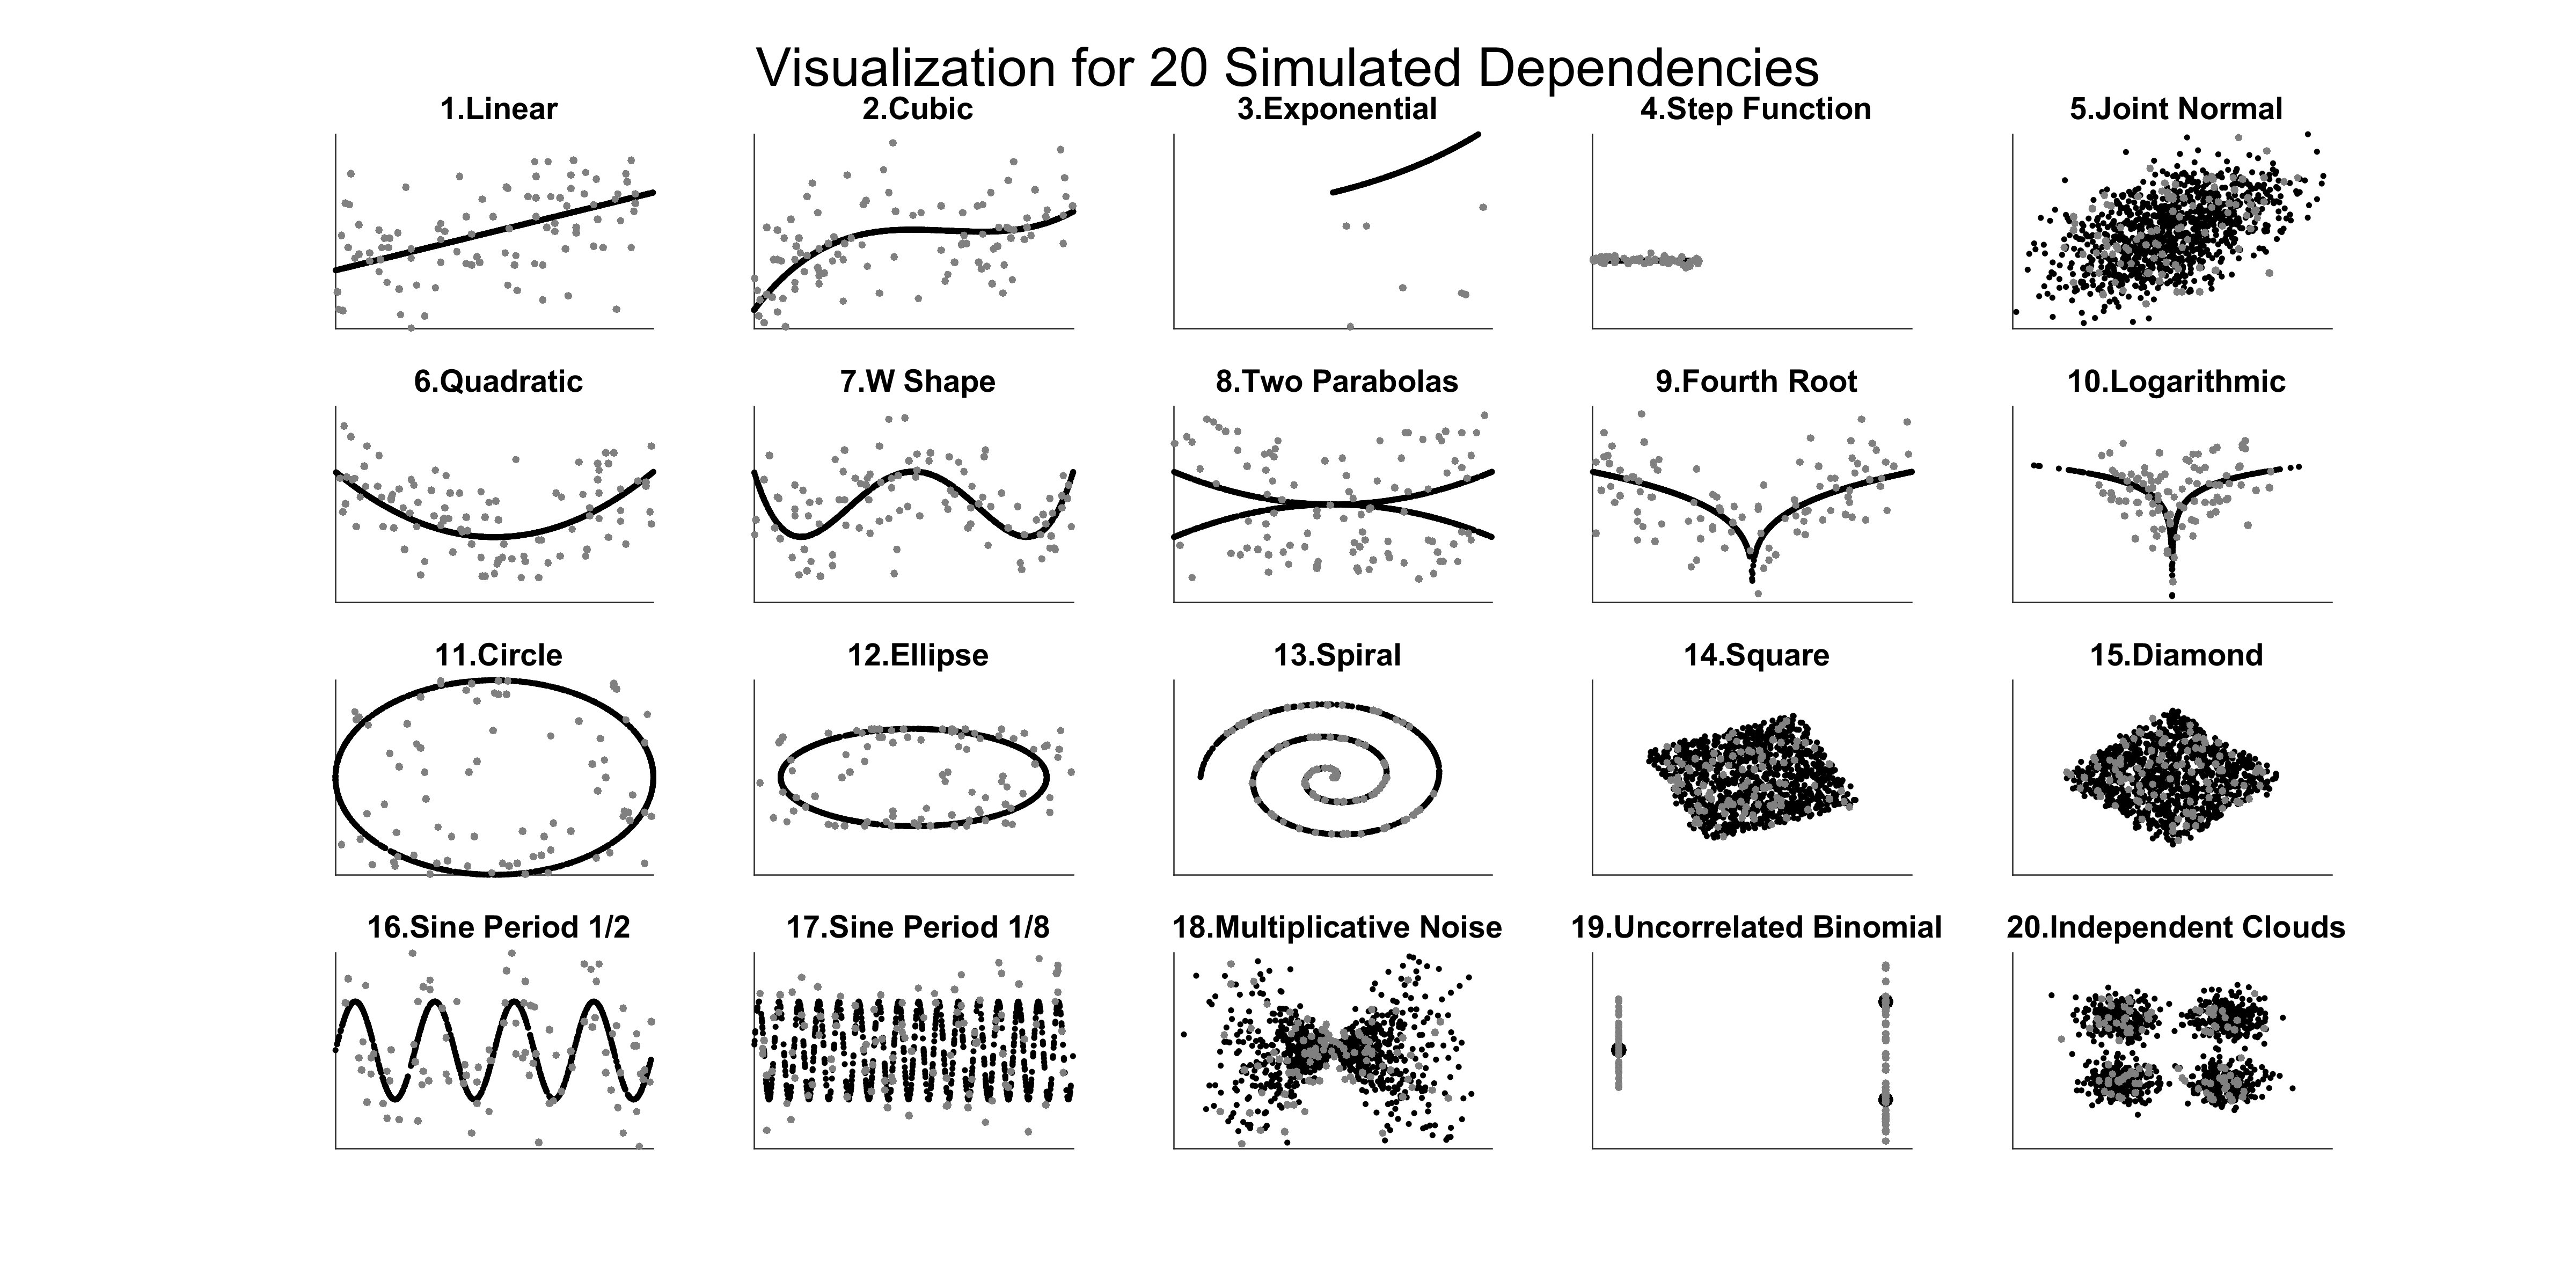
\includegraphics[trim={5cm 1.5cm 4cm 0.5cm},clip, width=1.0\textwidth]{Figures/FigSimVisual}
\caption{Visualization of the $20$ dependencies at $D=D_{y}=1$. For each, $n=100$ points are sampled with noise ($c=1$) to show the actual sample data used for 1-dimensional settings (gray dots). For comparison purposes, $n=1000$ points are sampled without noise ($c=0$) to highlight each underlying dependency (black dots).
}
\label{f:dependencies}
\end{figure}

\begin{figure}[htbp]
\vspace{-50pt}
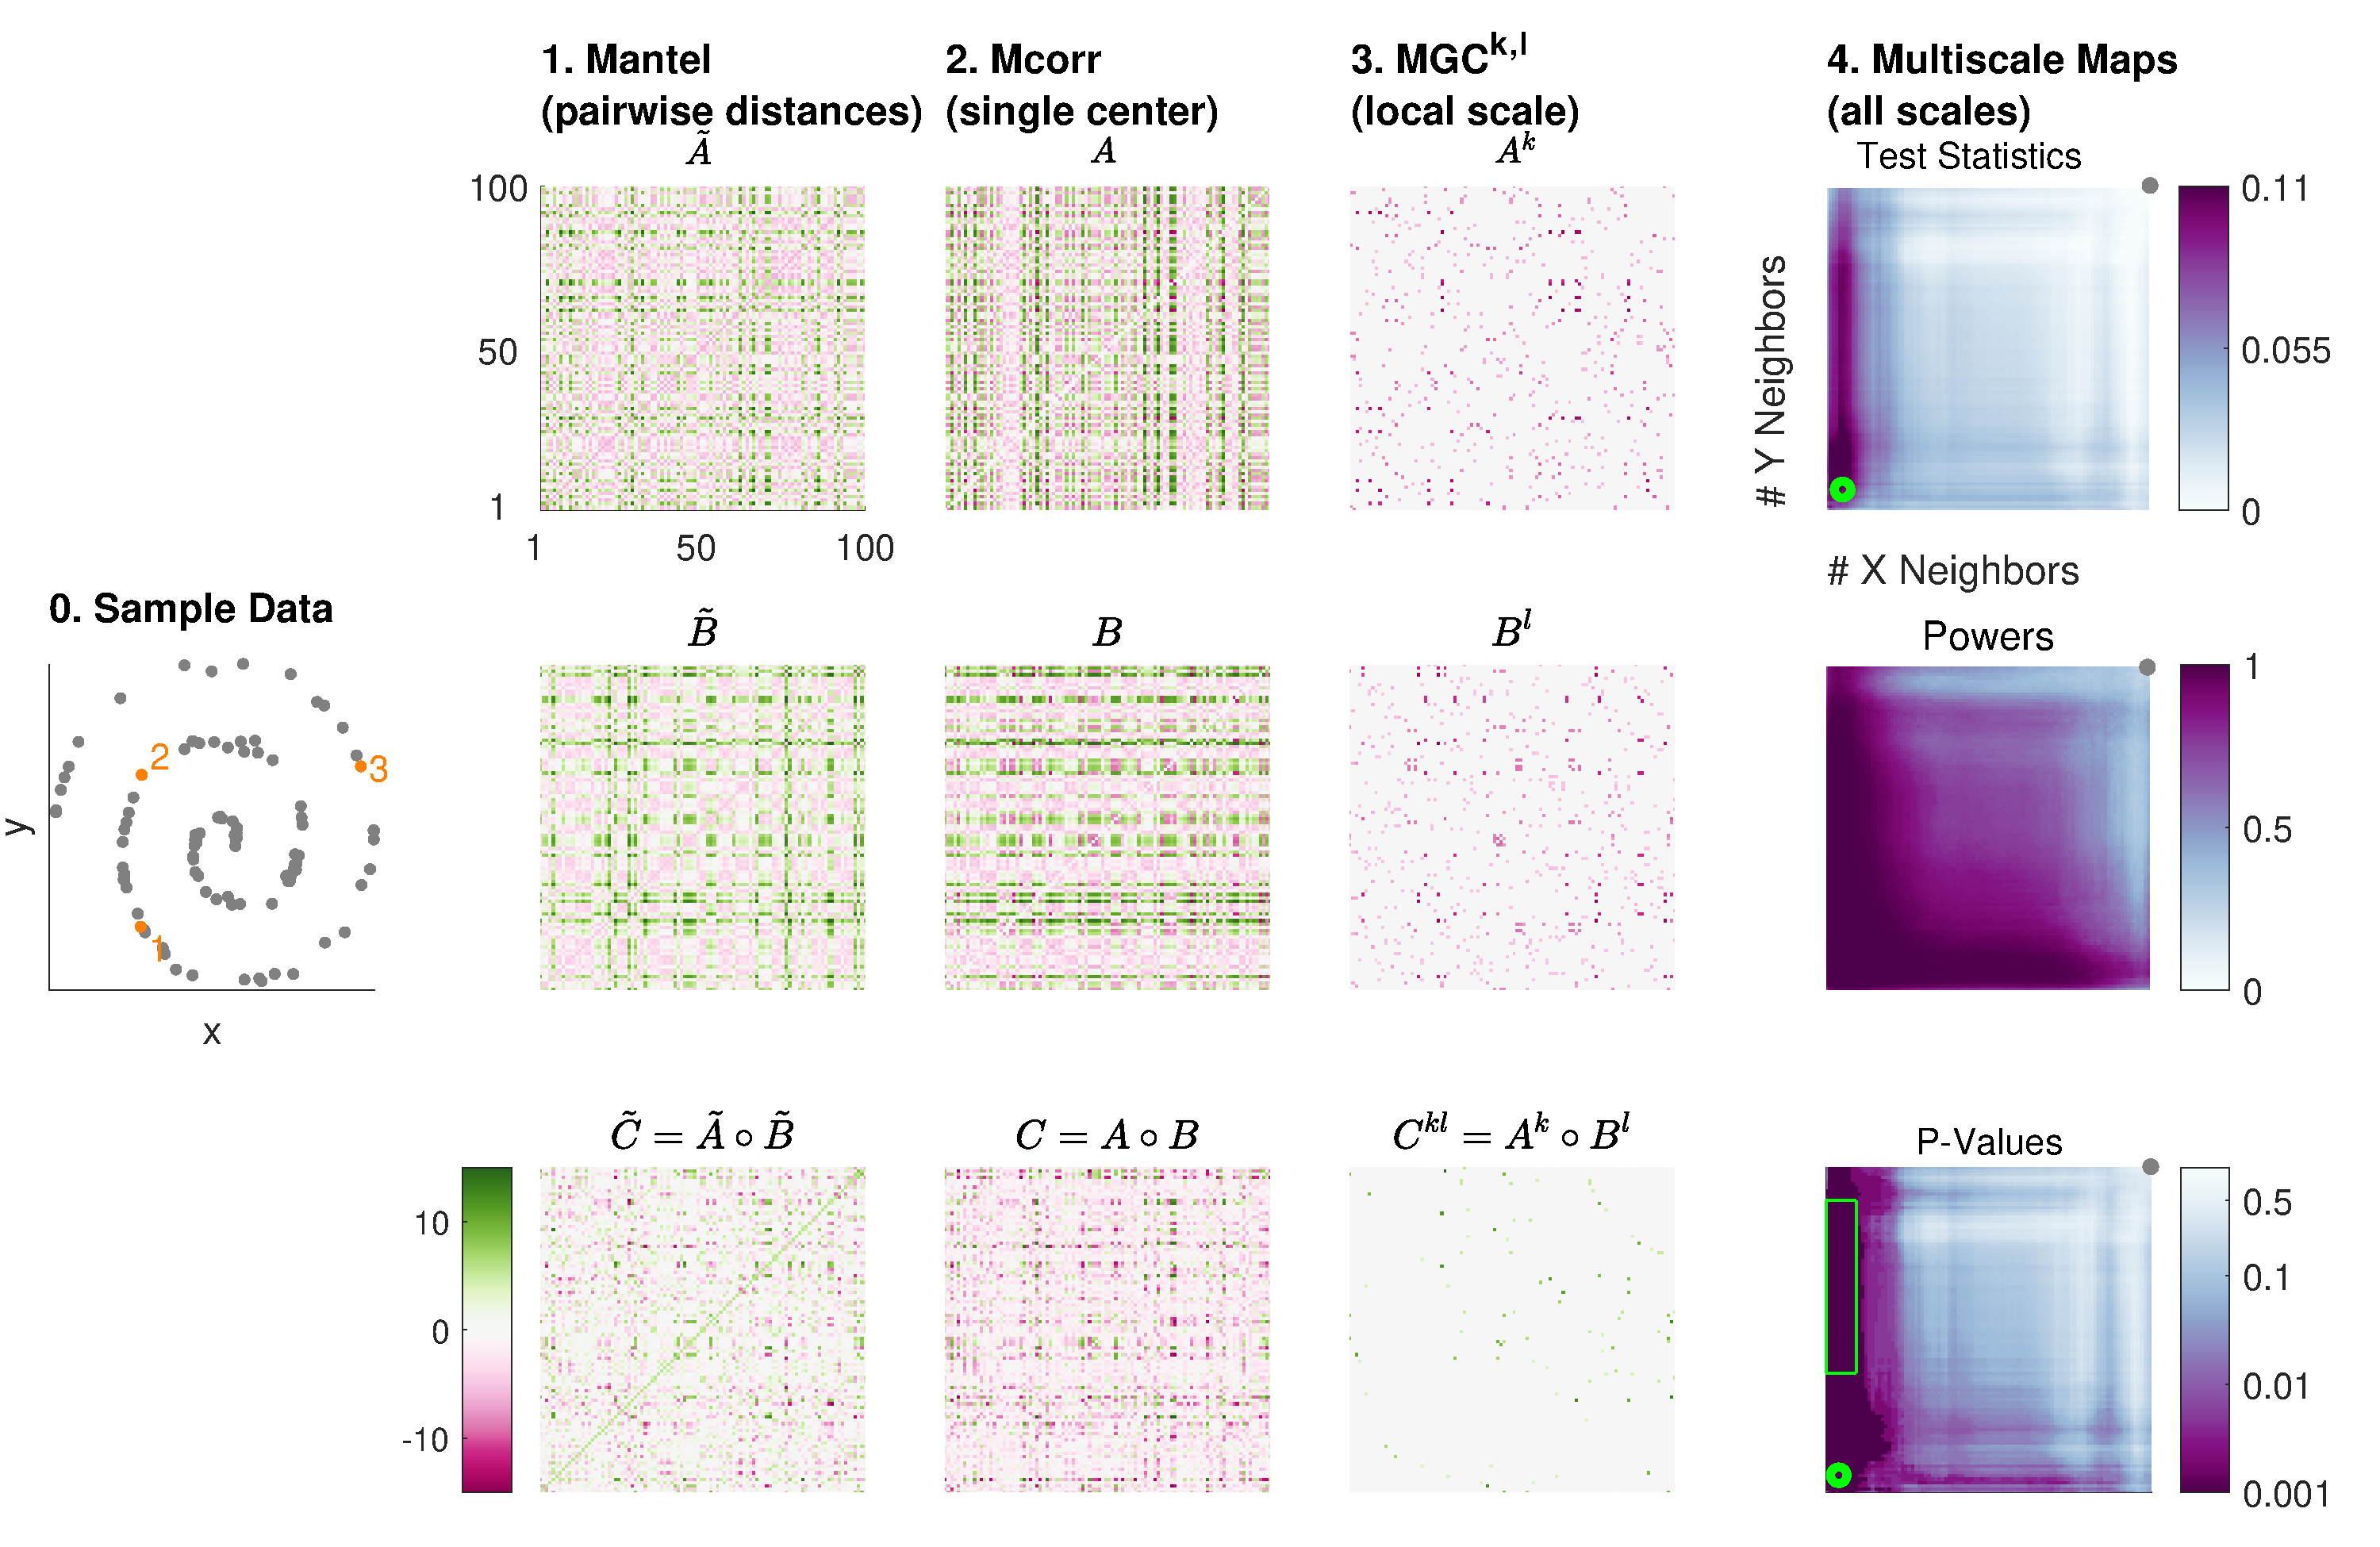
\includegraphics[width=1.0\textwidth,trim={0 0 0.75cm 0},clip]{Figures/FigA}
\setlength{\tabcolsep}{10pt} % Default value: 6pt
\begin{tabular}{r r r r}
\multicolumn{1}{l}{{\small \textbf{6. Table}}} & & & \\
$\delta_x$(1,2)   & \hspace{1.5em} \color{magenta}-2.03  & \hspace{3.5em} \color{magenta}-1.93  &  \hspace{3.0em} \color{magenta}-1.93  \\ 
 $\delta_y$(1,2) & \color{magenta}-2.30 & \color{magenta}-2.30 & \color{magenta}-2.30  \\ 
 $\delta_x \times \delta_y$ & \color{green}4.67 & \color{green}4.44 & \color{green}4.44  \\ 
 
\hline

 $\delta_x$(2,3) & \color{green}2.53 & \color{green}2.59 & 0.00  \\ 
 $\delta_y$(2,3) &  \color{magenta}-1.36 & \color{magenta}-2.03 & 0.00  \\ 
 $\delta_x \times \delta_y$ & \color{magenta}-3.43 & \color{magenta}-5.26 & 0.00  \\ 

\hline
 $\sum{\delta_x \times \delta_y}$ & \color{magenta}-502.61   & \color{green}92.95 & \color{green}301.33  \\ 
 test statistic &  \color{magenta}-0.02  & 0.00 & \color{green}0.10  \\  
\end{tabular}

\begin{tikzpicture}[remember picture,overlay]
\node[xshift=-5.2cm,yshift=-0.2cm] at (current page.east){%
    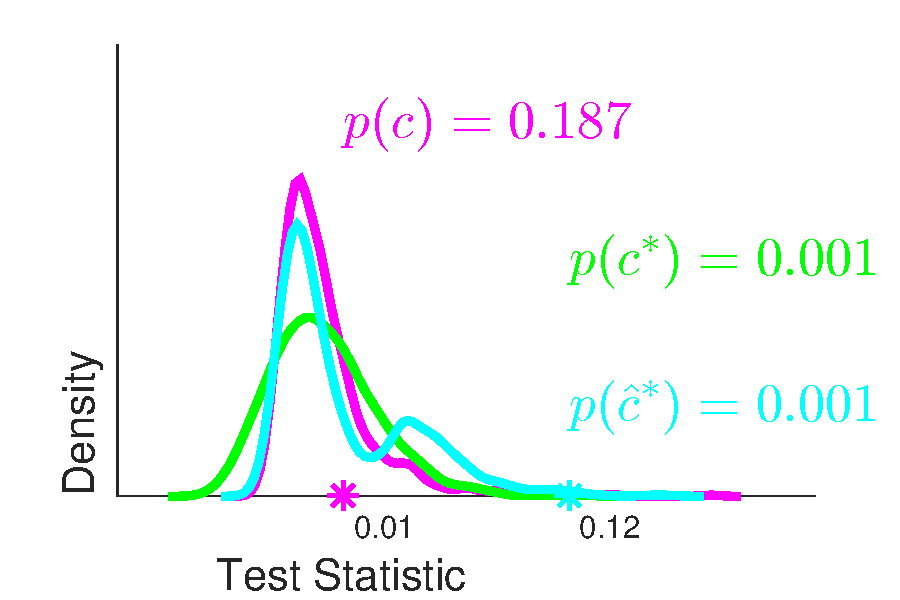
\includegraphics[width=0.35\textwidth,trim={1.5cm 0cm 1.8cm 0},clip]{Figures/FigB}};
  %\node[anchor=east,inner sep=0pt] at ($(current page.east)-(10cm,10cm)$) {
   %  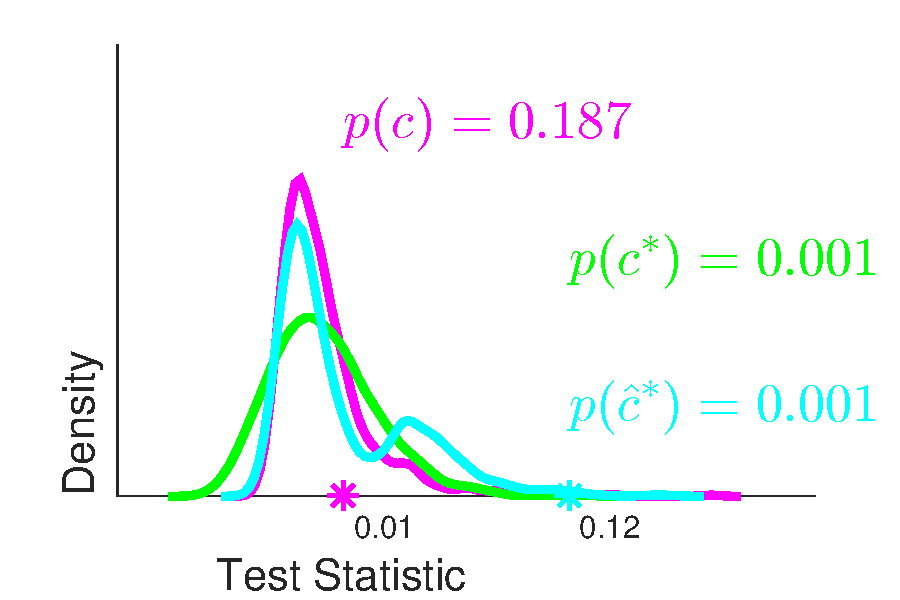
\includegraphics[width=0.3\textwidth]{Figures/FigB}
  %};
\end{tikzpicture}
\caption{
Schematic  and table demonstrating the ability of Multiscale Generalized Correlation (\Mgc) to detect dependence in nonlinear settings. 
\textbf{0.} 100 pairs of observations $(x_i,y_i)$ are nonlinearly (spirally) dependent on one another.
% 
\textbf{1.} Choose a metric on $x$ and another on $y$, and compute all pairwise distances (centered by the overall means) for $x$ and $y$ yielding interpoint comparison matrices
 $\tilde{A}$ (top) and $\tilde{B}$ (middle), 
and their element-wise products $\tilde{C}=\tilde{A} \circ \tilde{B}$ (bottom), whose normalized sum is the  \Mantel~statistic \cite{Mantel1967} (bottom row of table).
% 
\textbf{2.} Single centering --- subtract the row-sums from $\tilde{A}$ and column-sums from $\tilde{B}$ to eliminate bias due to individual samples --- yields $A=\{a_{ij}\}$ and $B=\{b_{ij}\}$; the normalized sum of their  element-wise product  $C$ is equivalent to the  \Mcorr~statistic \cite{SzekelyRizzo2013a}.
% 
\textbf{3.} Given a local scale, for example, $k=l=4$ here, yields $A^{k}$, $B^{l}$, and $C^{kl}$.  All these test statistics are normalized sums of the element-wise products. The fact that \Mgc~yields a $C^{kl}$ matrix that is all positive, whereas the others yield $C$ matrices with both positive and negative values, suggest that \Mgc~will correctly report a large test statistic here, resulting in a small p-value.
\textbf{4.} Compute the test statistics (top), power (middle), and p-value (bottom) for all local scales, resulting in multiscale maps that reveal the scales of dependency. Green dots show the location of optimal local correlation determined by Sample \Mgc~, and the green box shows the informative scales via the p-value map.
\textbf{5.} Report the corresponding observed test statistics and p-values, and discover the informative scales (green rectangle in  p-value map) by Sample \Mgc.  
Whereas \Mcorr, the global test, has very low power (magenta dot in  p-value map) and therefore yields a small statistic and a non-significant p-value ($0.257$),  there are many local scales that achieve nearly perfect power, so both Oracle and Sample \Mgc~($\GG^{*}$ and $\hat{\GG}^{*}$) obtain large test statistics and highly significant p-values ($\approx 0.001$) and reveal the scales of dependency. 
\textbf{6.} Numerical demonstration of how \Mgc~is able to detect dependence even in highly nonlinear and low-sample size settings. The three colored points in the scatter plot indicate the three points considered in this table. 
The global methods fail to detect significant dependence since they consider all pairs, including the non-local ones, which \emph{negatively} impact the degree of dependence estimated.
\Mgc~only considers pairs that are jointly local (such as $(1,2)$), while discarding other pairs (such as $(2,3)$). 
}
\label{f:schematic}
\end{figure}

\begin{figure}[htbp]
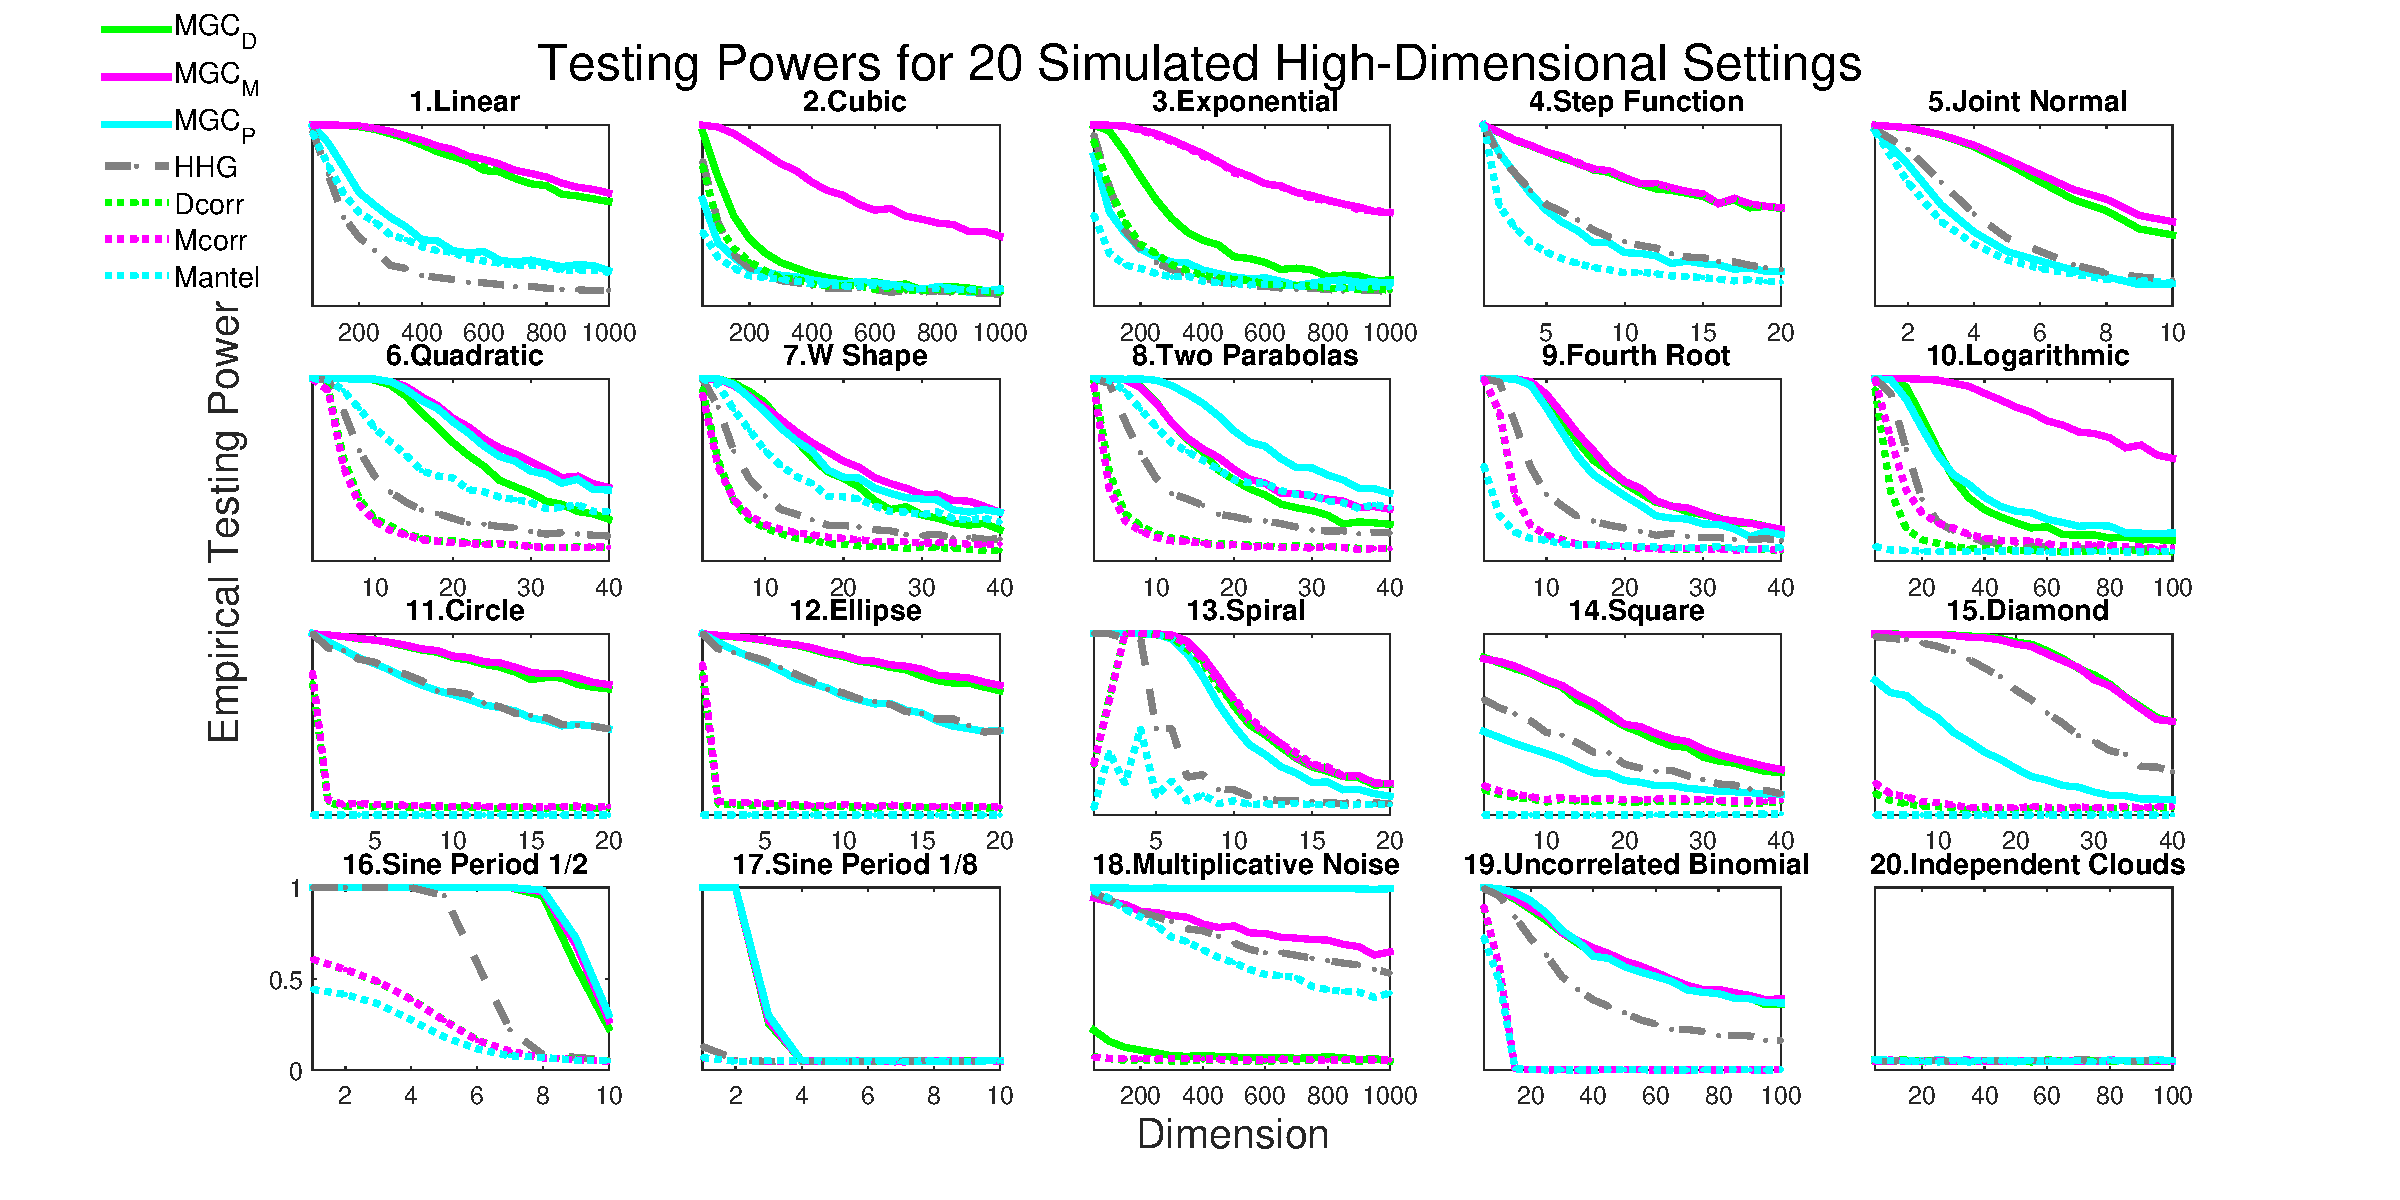
\includegraphics[width=1.0\textwidth,trim={0 0.5cm 4cm 0},clip]{Figures/FigHDPowerAll}
\caption{Power of different methods for $20$ different dependence settings, estimated by Monte Carlo independence tests (see Algorithm \ref{alg:power} for details). It includes eight different tests: \Mcorr, \Dcorr, and \Mantel~(gray solid, dashed, and dashdot lines, respectively), their corresponding Oracle \Mgc~counterparts, \Mgcm, \Mgcd, \Mgcp~(green with same line styles), Sample \Mgc~applied to \Mcorr~(cyan solid), and \Hhg~(gray dotted line). 
Each panel shows the testing power at significance level $\alpha=0.05$ versus the dimensionality of $\mb{x}$'s, for $n=100$ samples. 
Excluding the independent setting (\#20), for which all methods yield power $0.05$, as they should, Oracle \Mgc~empirically achieves similar or better power than the respective global counterpart. In particular, Sample \Mgc~is very close to Oracle \Mgcm, and overall dominates existing approaches for almost all settings and all dimensions, including \Hhg~\cite{HellerGorfine2013}, another state-of-the-art method. Note that \Mgc~is always plotted ``on top'' of the global variants if there is overlap, therefore, some of the global variants are not always visible from the display.}
\label{f:nDAll}
\end{figure}

\begin{figure}[htbp]
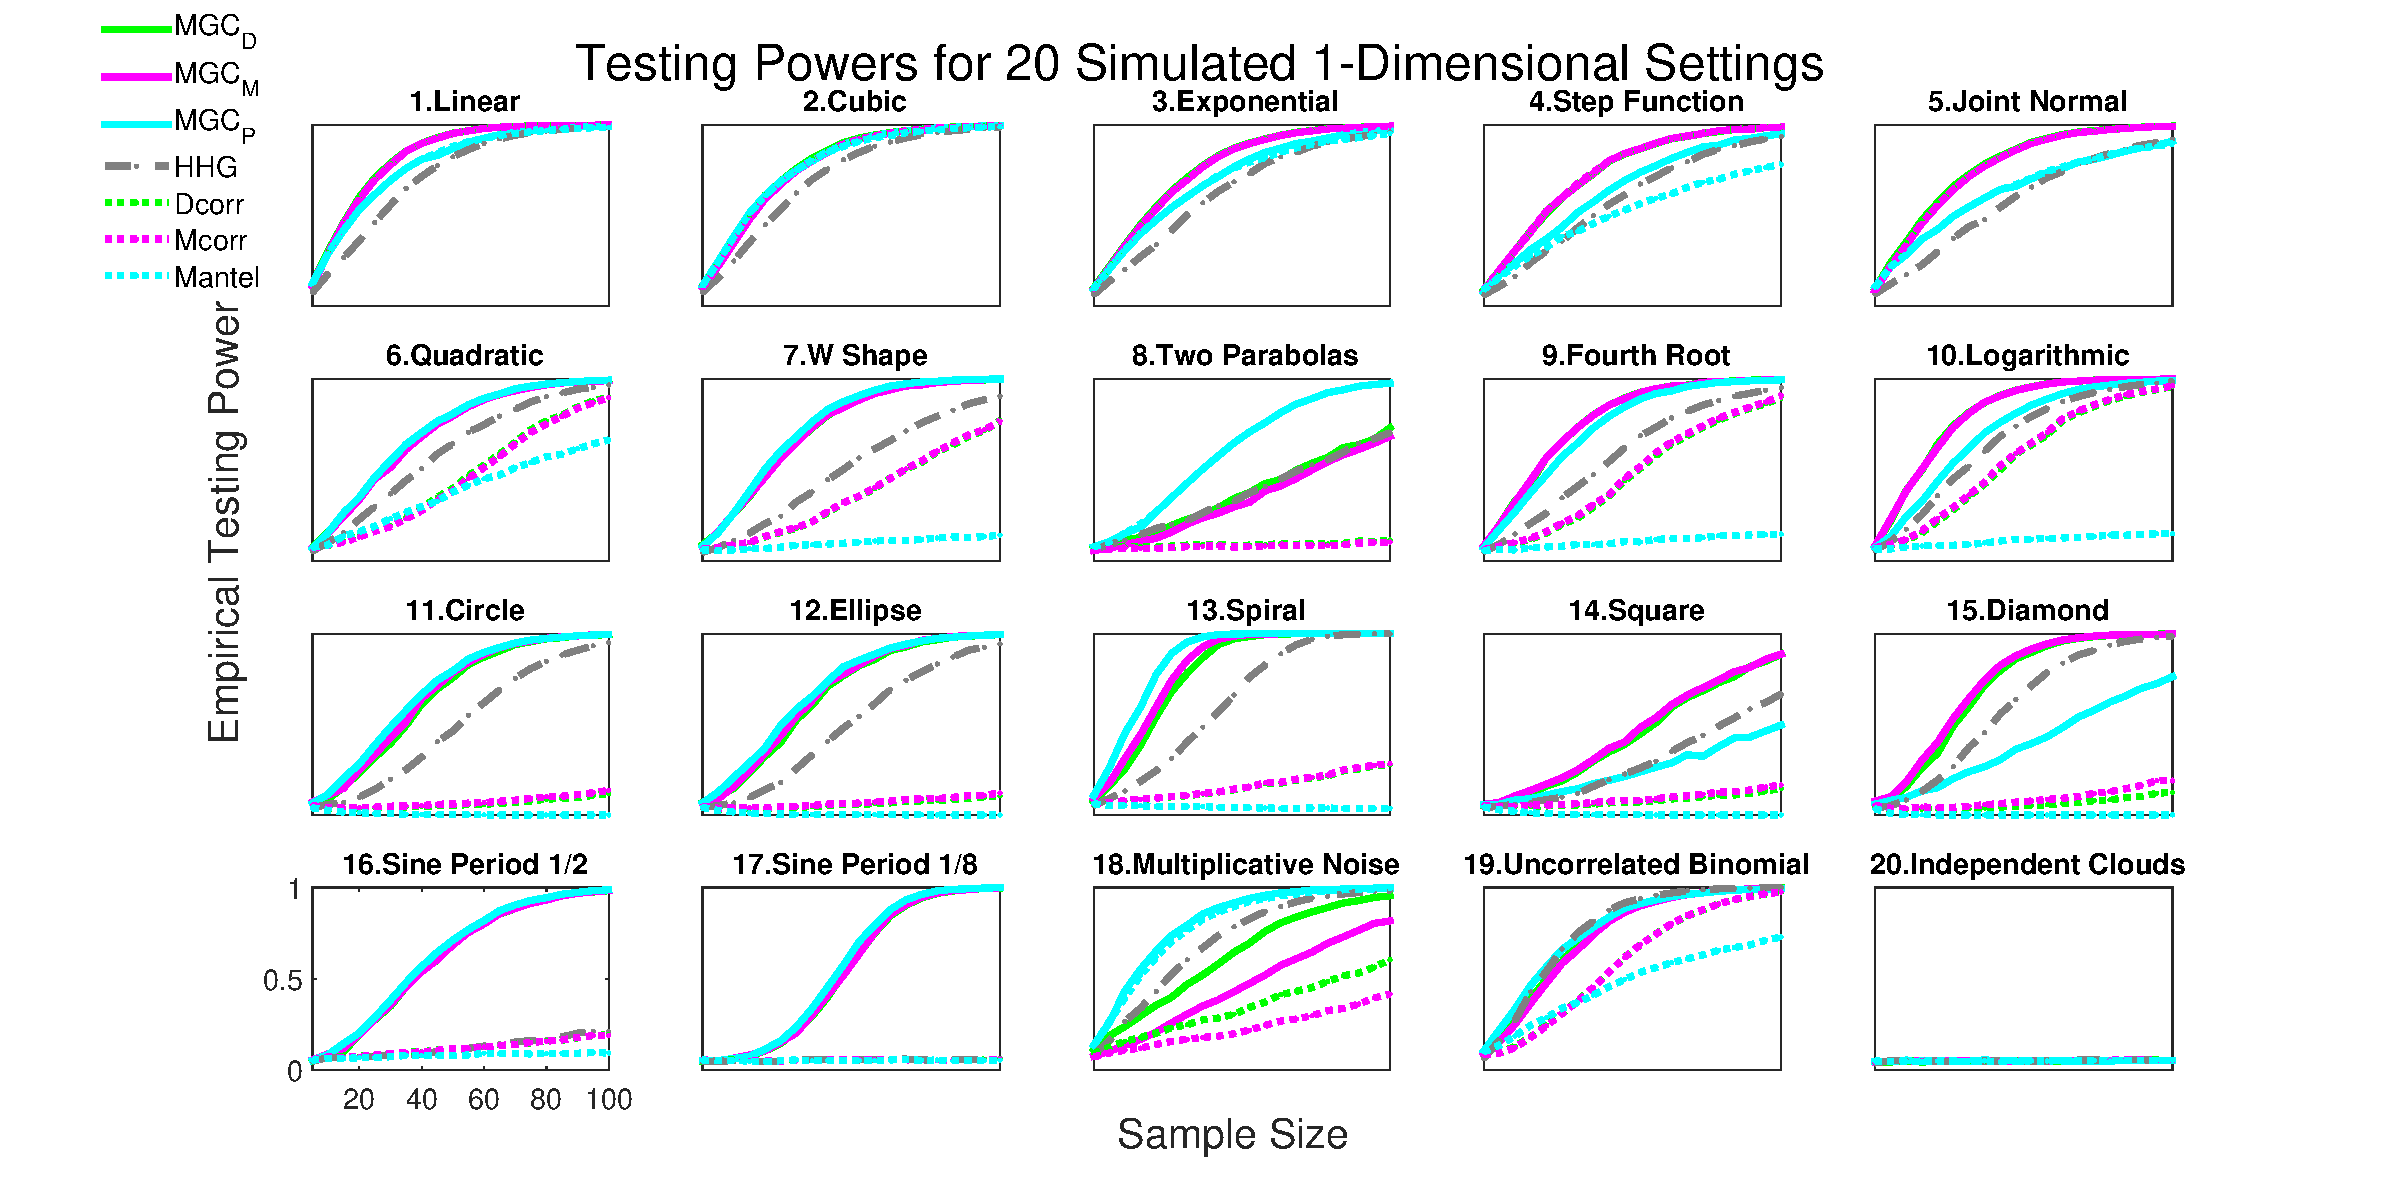
\includegraphics[width=1.0\textwidth,trim={0 0.5cm 4cm 0},clip]{Figures/Fig1DPowerAll}
\caption{
The same power plots as in Figure~\ref{f:nDAll}, except the $20$ dependence settings are one-dimensional with noise, and the x-axis is increasing sample size.
Each panel shows the testing power on the abscissa at a significance level $\alpha=0.05$, and sample size on the ordinate.
Again, Oracle \Mgc~empirically achieves similar or better power than the previous state of the art approaches for all sample sizes on almost all problems, with Sample \Mgc~being very close to Oracle \Mgc~and overall superior to other benchmarks.}
\label{f:1DAll}
\end{figure}

\begin{figure}
  \centering
  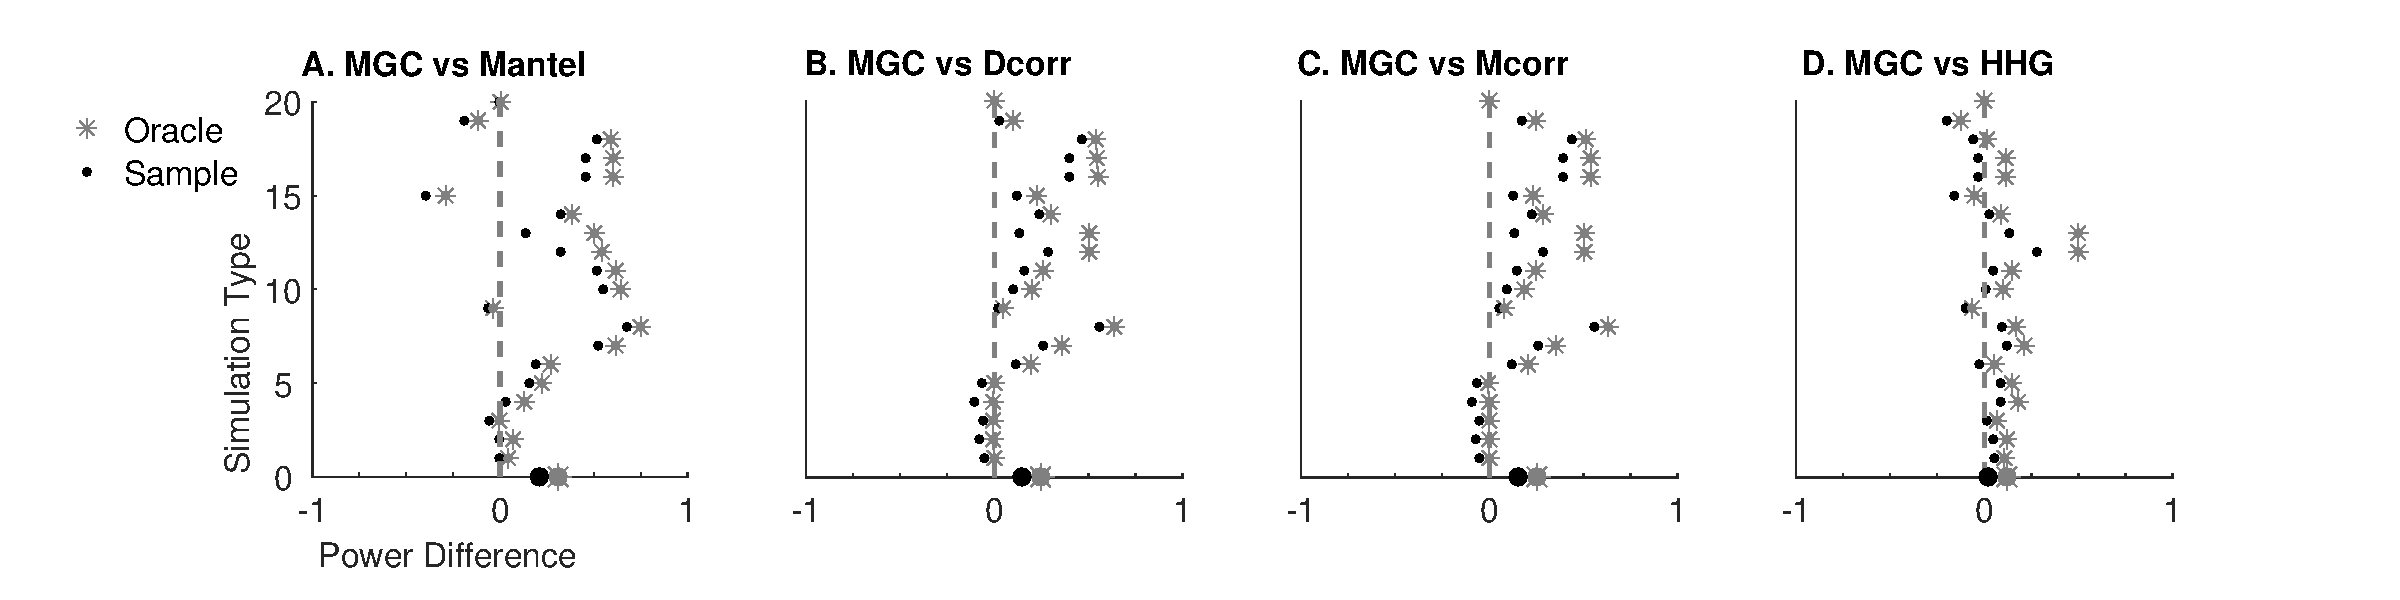
\includegraphics[width=1.0\textwidth,trim={3.5cm 0 3.5cm 0},clip]{Figures/Fig1DPowerMGCM}
  \caption{The same summary figure as Figure~\ref{f:nDSummary}, but based on the testing power of the $20$ one-dimensional simulation settings in Figure~\ref{f:1DAll}, averaged over sample size. 
  \Mgc~is again the most superior methods, exhibiting mean power slightly over \Hhg~for most settings, and very significant advantage over \Mantel, \Dcorr, \Mcorr~for most nonlinear dependencies.}
\label{f:1DSummary}
\end{figure}


\begin{figure}[htbp]
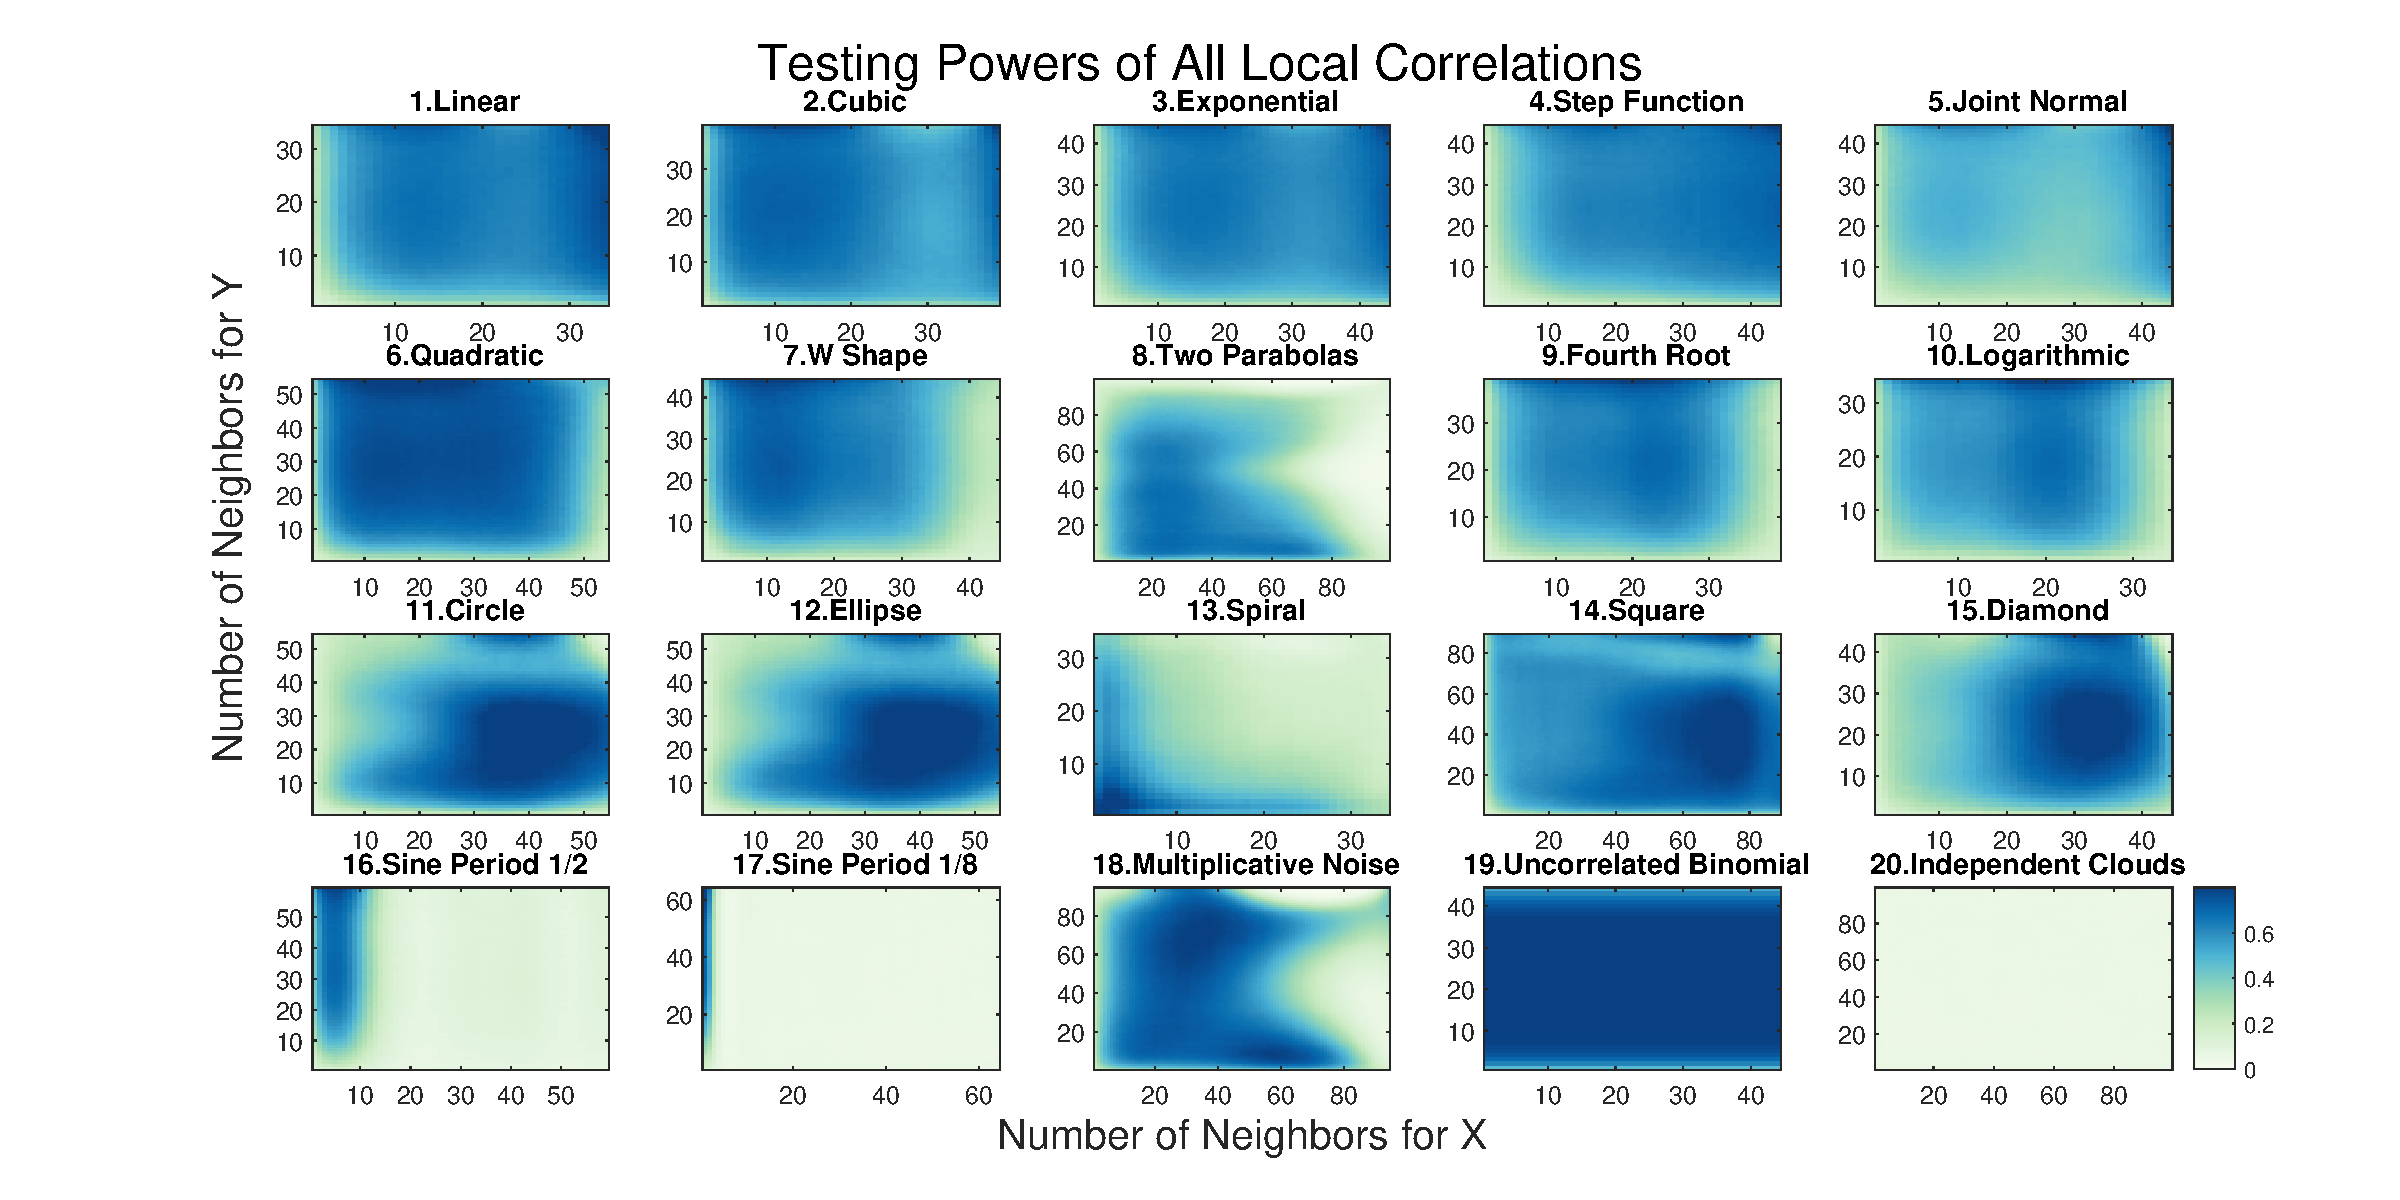
\includegraphics[width=1.0\textwidth,trim={3cm 0.5cm 2.5cm 0.5cm},clip]{Figures/Fig1DHeat}
\caption{Multiscale Power Maps indicating the influence of neighborhood size on \Mgc~testing power, for the one-dimensional simulations in Figure~\ref{f:1DAll}. For each simulation,  the sample size is $n=60$, and the significance level is $\alpha=0.05$. It has similar behavior and interpretation as the high-dimensional power maps in Figure~\ref{f:powermaps}.}
\label{f:powermaps1}
\end{figure}

\end{document}